\documentclass[twoside]{book}

% Packages required by doxygen
\usepackage{calc}
\usepackage{doxygen}
\usepackage{graphicx}
\usepackage[utf8]{inputenc}
\usepackage{makeidx}
\usepackage{multicol}
\usepackage{multirow}
\usepackage{textcomp}
\usepackage[table]{xcolor}

% Font selection
\usepackage[T1]{fontenc}
\usepackage{mathptmx}
\usepackage[scaled=.90]{helvet}
\usepackage{courier}
\usepackage{amssymb}
\usepackage{sectsty}
\renewcommand{\familydefault}{\sfdefault}
\allsectionsfont{%
  \fontseries{bc}\selectfont%
  \color{darkgray}%
}
\renewcommand{\DoxyLabelFont}{%
  \fontseries{bc}\selectfont%
  \color{darkgray}%
}

% Page & text layout
\usepackage{geometry}
\geometry{%
  a4paper,%
  top=2.5cm,%
  bottom=2.5cm,%
  left=2.5cm,%
  right=2.5cm%
}
\tolerance=750
\hfuzz=15pt
\hbadness=750
\setlength{\emergencystretch}{15pt}
\setlength{\parindent}{0cm}
\setlength{\parskip}{0.2cm}
\makeatletter
\renewcommand{\paragraph}{%
  \@startsection{paragraph}{4}{0ex}{-1.0ex}{1.0ex}{%
    \normalfont\normalsize\bfseries\SS@parafont%
  }%
}
\renewcommand{\subparagraph}{%
  \@startsection{subparagraph}{5}{0ex}{-1.0ex}{1.0ex}{%
    \normalfont\normalsize\bfseries\SS@subparafont%
  }%
}
\makeatother

% Headers & footers
\usepackage{fancyhdr}
\pagestyle{fancyplain}
\fancyhead[LE]{\fancyplain{}{\bfseries\thepage}}
\fancyhead[CE]{\fancyplain{}{}}
\fancyhead[RE]{\fancyplain{}{\bfseries\leftmark}}
\fancyhead[LO]{\fancyplain{}{\bfseries\rightmark}}
\fancyhead[CO]{\fancyplain{}{}}
\fancyhead[RO]{\fancyplain{}{\bfseries\thepage}}
\fancyfoot[LE]{\fancyplain{}{}}
\fancyfoot[CE]{\fancyplain{}{}}
\fancyfoot[RE]{\fancyplain{}{\bfseries\scriptsize Generated on Thu Jun 30 2016 14\-:00\-:35 for Zero\-M\-Q Component Model by Doxygen }}
\fancyfoot[LO]{\fancyplain{}{\bfseries\scriptsize Generated on Thu Jun 30 2016 14\-:00\-:35 for Zero\-M\-Q Component Model by Doxygen }}
\fancyfoot[CO]{\fancyplain{}{}}
\fancyfoot[RO]{\fancyplain{}{}}
\renewcommand{\footrulewidth}{0.4pt}
\renewcommand{\chaptermark}[1]{%
  \markboth{#1}{}%
}
\renewcommand{\sectionmark}[1]{%
  \markright{\thesection\ #1}%
}

% Indices & bibliography
\usepackage{natbib}
\usepackage[titles]{tocloft}
\setcounter{tocdepth}{3}
\setcounter{secnumdepth}{5}
\makeindex

% Hyperlinks (required, but should be loaded last)
\usepackage{ifpdf}
\ifpdf
  \usepackage[pdftex,pagebackref=true]{hyperref}
\else
  \usepackage[ps2pdf,pagebackref=true]{hyperref}
\fi
\hypersetup{%
  colorlinks=true,%
  linkcolor=blue,%
  citecolor=blue,%
  unicode%
}

% Custom commands
\newcommand{\clearemptydoublepage}{%
  \newpage{\pagestyle{empty}\cleardoublepage}%
}


%===== C O N T E N T S =====

\begin{document}

% Titlepage & ToC
\hypersetup{pageanchor=false}
\pagenumbering{roman}
\begin{titlepage}
\vspace*{7cm}
\begin{center}%
{\Large Zero\-M\-Q Component Model }\\
\vspace*{1cm}
{\large Generated by Doxygen 1.8.6}\\
\vspace*{0.5cm}
{\small Thu Jun 30 2016 14:00:35}\\
\end{center}
\end{titlepage}
\clearemptydoublepage
\tableofcontents
\clearemptydoublepage
\pagenumbering{arabic}
\hypersetup{pageanchor=true}

%--- Begin generated contents ---
\chapter{Namespace Index}
\section{Namespace List}
Here is a list of all namespaces with brief descriptions\-:\begin{DoxyCompactList}
\item\contentsline{section}{\hyperlink{namespacezcm}{zcm} }{\pageref{namespacezcm}}{}
\end{DoxyCompactList}

\chapter{Hierarchical Index}
\section{Class Hierarchy}
This inheritance list is sorted roughly, but not completely, alphabetically\+:\begin{DoxyCompactList}
\item \contentsline{section}{zcm\+:\+:Actor}{\pageref{classzcm_1_1Actor}}{}
\item \contentsline{section}{zcm\+:\+:Base\+\_\+\+Operation}{\pageref{classzcm_1_1Base__Operation}}{}
\begin{DoxyCompactList}
\item \contentsline{section}{zcm\+:\+:Server\+\_\+\+Operation}{\pageref{classzcm_1_1Server__Operation}}{}
\item \contentsline{section}{zcm\+:\+:Subscriber\+\_\+\+Operation}{\pageref{classzcm_1_1Subscriber__Operation}}{}
\item \contentsline{section}{zcm\+:\+:Timer\+\_\+\+Operation}{\pageref{classzcm_1_1Timer__Operation}}{}
\end{DoxyCompactList}
\item \contentsline{section}{zcm\+:\+:Client}{\pageref{classzcm_1_1Client}}{}
\item \contentsline{section}{zcm\+:\+:Component}{\pageref{classzcm_1_1Component}}{}
\item \contentsline{section}{zcm\+:\+:Operation\+\_\+\+Queue}{\pageref{classzcm_1_1Operation__Queue}}{}
\item \contentsline{section}{zcm\+:\+:Operation\+\_\+\+Queue\+:\+:Priority\+Ordering}{\pageref{structzcm_1_1Operation__Queue_1_1PriorityOrdering}}{}
\item \contentsline{section}{zcm\+:\+:Publisher}{\pageref{classzcm_1_1Publisher}}{}
\item \contentsline{section}{zcm\+:\+:Server}{\pageref{classzcm_1_1Server}}{}
\item \contentsline{section}{zcm\+:\+:Subscriber}{\pageref{classzcm_1_1Subscriber}}{}
\item \contentsline{section}{zcm\+:\+:Timer}{\pageref{classzcm_1_1Timer}}{}
\end{DoxyCompactList}

\chapter{Class Index}
\section{Class List}
Here are the classes, structs, unions and interfaces with brief descriptions\+:\begin{DoxyCompactList}
\item\contentsline{section}{\hyperlink{classzcm_1_1Base__Operation}{zcm\+::\+Base\+\_\+\+Operation} \\*Base Operation class }{\pageref{classzcm_1_1Base__Operation}}{}
\item\contentsline{section}{\hyperlink{classzcm_1_1Client}{zcm\+::\+Client} \\*\hyperlink{classzcm_1_1Client}{Client} class }{\pageref{classzcm_1_1Client}}{}
\item\contentsline{section}{\hyperlink{classzcm_1_1Component}{zcm\+::\+Component} \\*\hyperlink{classzcm_1_1Component}{Component} class }{\pageref{classzcm_1_1Component}}{}
\item\contentsline{section}{\hyperlink{classzcm_1_1Operation__Queue}{zcm\+::\+Operation\+\_\+\+Queue} \\*\hyperlink{classzcm_1_1Operation__Queue}{Operation\+\_\+\+Queue} class }{\pageref{classzcm_1_1Operation__Queue}}{}
\item\contentsline{section}{\hyperlink{structzcm_1_1Operation__Queue_1_1PriorityOrdering}{zcm\+::\+Operation\+\_\+\+Queue\+::\+Priority\+Ordering} }{\pageref{structzcm_1_1Operation__Queue_1_1PriorityOrdering}}{}
\item\contentsline{section}{\hyperlink{classzcm_1_1Publisher}{zcm\+::\+Publisher} \\*\hyperlink{classzcm_1_1Publisher}{Publisher} class }{\pageref{classzcm_1_1Publisher}}{}
\item\contentsline{section}{\hyperlink{classzcm_1_1Server}{zcm\+::\+Server} \\*\hyperlink{classzcm_1_1Server}{Server} class }{\pageref{classzcm_1_1Server}}{}
\item\contentsline{section}{\hyperlink{classzcm_1_1Server__Operation}{zcm\+::\+Server\+\_\+\+Operation} \\*\hyperlink{classzcm_1_1Server}{Server} Operation class }{\pageref{classzcm_1_1Server__Operation}}{}
\item\contentsline{section}{\hyperlink{classzcm_1_1Subscriber}{zcm\+::\+Subscriber} \\*\hyperlink{classzcm_1_1Subscriber}{Subscriber} class }{\pageref{classzcm_1_1Subscriber}}{}
\item\contentsline{section}{\hyperlink{classzcm_1_1Subscriber__Operation}{zcm\+::\+Subscriber\+\_\+\+Operation} \\*\hyperlink{classzcm_1_1Subscriber}{Subscriber} Operation class }{\pageref{classzcm_1_1Subscriber__Operation}}{}
\item\contentsline{section}{\hyperlink{classzcm_1_1Timer}{zcm\+::\+Timer} \\*\hyperlink{classzcm_1_1Timer}{Timer} class }{\pageref{classzcm_1_1Timer}}{}
\item\contentsline{section}{\hyperlink{classzcm_1_1Timer__Operation}{zcm\+::\+Timer\+\_\+\+Operation} \\*\hyperlink{classzcm_1_1Timer}{Timer} Operation class }{\pageref{classzcm_1_1Timer__Operation}}{}
\end{DoxyCompactList}

\chapter{File Index}
\section{File List}
Here is a list of all documented files with brief descriptions\+:\begin{DoxyCompactList}
\item\contentsline{section}{/home/pranav/\+Repositories/zmq-\/comm/include/{\bfseries client.\+hpp} }{\pageref{client_8hpp}}{}
\item\contentsline{section}{/home/pranav/\+Repositories/zmq-\/comm/include/{\bfseries component.\+hpp} }{\pageref{component_8hpp}}{}
\item\contentsline{section}{/home/pranav/\+Repositories/zmq-\/comm/include/{\bfseries operation\+\_\+queue.\+hpp} }{\pageref{operation__queue_8hpp}}{}
\item\contentsline{section}{/home/pranav/\+Repositories/zmq-\/comm/include/{\bfseries operation\+\_\+types.\+hpp} }{\pageref{operation__types_8hpp}}{}
\item\contentsline{section}{/home/pranav/\+Repositories/zmq-\/comm/include/{\bfseries publisher.\+hpp} }{\pageref{publisher_8hpp}}{}
\item\contentsline{section}{/home/pranav/\+Repositories/zmq-\/comm/include/{\bfseries server.\+hpp} }{\pageref{server_8hpp}}{}
\item\contentsline{section}{/home/pranav/\+Repositories/zmq-\/comm/include/{\bfseries subscriber.\+hpp} }{\pageref{subscriber_8hpp}}{}
\item\contentsline{section}{/home/pranav/\+Repositories/zmq-\/comm/include/\hyperlink{timer_8hpp}{timer.\+hpp} \\*This file declares the \hyperlink{classTimer}{Timer} class }{\pageref{timer_8hpp}}{}
\item\contentsline{section}{/home/pranav/\+Repositories/zmq-\/comm/include/{\bfseries xml\+\_\+parser.\+hpp} }{\pageref{xml__parser_8hpp}}{}
\item\contentsline{section}{/home/pranav/\+Repositories/zmq-\/comm/src/\hyperlink{timer_8cpp}{timer.\+cpp} \\*This file contains definitions for the \hyperlink{classTimer}{Timer} class }{\pageref{timer_8cpp}}{}
\end{DoxyCompactList}

\chapter{Namespace Documentation}
\hypertarget{namespacezcm}{\section{zcm Namespace Reference}
\label{namespacezcm}\index{zcm@{zcm}}
}
\subsection*{Classes}
\begin{DoxyCompactItemize}
\item 
class \hyperlink{classzcm_1_1Actor}{Actor}
\begin{DoxyCompactList}\small\item\em \hyperlink{classzcm_1_1Actor}{Actor} class. \end{DoxyCompactList}\item 
class \hyperlink{classzcm_1_1Client}{Client}
\begin{DoxyCompactList}\small\item\em \hyperlink{classzcm_1_1Client}{Client} class. \end{DoxyCompactList}\item 
class \hyperlink{classzcm_1_1Component}{Component}
\begin{DoxyCompactList}\small\item\em \hyperlink{classzcm_1_1Component}{Component} class. \end{DoxyCompactList}\item 
class \hyperlink{classzcm_1_1Operation__Queue}{Operation\-\_\-\-Queue}
\begin{DoxyCompactList}\small\item\em \hyperlink{classzcm_1_1Operation__Queue}{Operation\-\_\-\-Queue} class. \end{DoxyCompactList}\item 
class \hyperlink{classzcm_1_1Base__Operation}{Base\-\_\-\-Operation}
\begin{DoxyCompactList}\small\item\em Base Operation class. \end{DoxyCompactList}\item 
class \hyperlink{classzcm_1_1Timer__Operation}{Timer\-\_\-\-Operation}
\begin{DoxyCompactList}\small\item\em \hyperlink{classzcm_1_1Timer}{Timer} Operation class. \end{DoxyCompactList}\item 
class \hyperlink{classzcm_1_1Subscriber__Operation}{Subscriber\-\_\-\-Operation}
\begin{DoxyCompactList}\small\item\em \hyperlink{classzcm_1_1Subscriber}{Subscriber} Operation class. \end{DoxyCompactList}\item 
class \hyperlink{classzcm_1_1Server__Operation}{Server\-\_\-\-Operation}
\begin{DoxyCompactList}\small\item\em \hyperlink{classzcm_1_1Server}{Server} Operation class. \end{DoxyCompactList}\item 
class \hyperlink{classzcm_1_1Publisher}{Publisher}
\begin{DoxyCompactList}\small\item\em \hyperlink{classzcm_1_1Publisher}{Publisher} class. \end{DoxyCompactList}\item 
class \hyperlink{classzcm_1_1Server}{Server}
\begin{DoxyCompactList}\small\item\em \hyperlink{classzcm_1_1Server}{Server} class. \end{DoxyCompactList}\item 
class \hyperlink{classzcm_1_1Subscriber}{Subscriber}
\begin{DoxyCompactList}\small\item\em \hyperlink{classzcm_1_1Subscriber}{Subscriber} class. \end{DoxyCompactList}\item 
class \hyperlink{classzcm_1_1Timer}{Timer}
\begin{DoxyCompactList}\small\item\em \hyperlink{classzcm_1_1Timer}{Timer} class. \end{DoxyCompactList}\end{DoxyCompactItemize}

\chapter{Class Documentation}
\hypertarget{classzcm_1_1Actor}{\section{zcm\-:\-:Actor Class Reference}
\label{classzcm_1_1Actor}\index{zcm\-::\-Actor@{zcm\-::\-Actor}}
}


\hyperlink{classzcm_1_1Actor}{Actor} class.  




{\ttfamily \#include $<$actor.\-hpp$>$}

\subsection*{Public Member Functions}
\begin{DoxyCompactItemize}
\item 
void \hyperlink{classzcm_1_1Actor_a28d09bc2ef3635296c988a2b32d10c0b}{configure} (std\-::string configuration\-\_\-file)
\begin{DoxyCompactList}\small\item\em Configure the component\-\_\-instances vector. \end{DoxyCompactList}\item 
void \hyperlink{classzcm_1_1Actor_a5d968074bf915f3e021cc287bff27879}{run} ()
\begin{DoxyCompactList}\small\item\em Spawn all component instances. \end{DoxyCompactList}\item 
std\-::string \hyperlink{classzcm_1_1Actor_ae81346a318c26d68a5b78848ead2518f}{get\-\_\-name} ()
\begin{DoxyCompactList}\small\item\em Get actor name. \end{DoxyCompactList}\end{DoxyCompactItemize}
\subsection*{Private Attributes}
\begin{DoxyCompactItemize}
\item 
std\-::string \hyperlink{classzcm_1_1Actor_a2b0816bbe28c8f96fa882b625be004ee}{name}
\item 
std\-::vector$<$ \hyperlink{classzcm_1_1Component}{Component} $\ast$ $>$ \hyperlink{classzcm_1_1Actor_abb7a2cdfc286c8821ac6f9ad3da40a49}{component\-\_\-instances}
\end{DoxyCompactItemize}


\subsection{Detailed Description}
\hyperlink{classzcm_1_1Actor}{Actor} class. 

\subsection{Member Function Documentation}
\hypertarget{classzcm_1_1Actor_a28d09bc2ef3635296c988a2b32d10c0b}{\index{zcm\-::\-Actor@{zcm\-::\-Actor}!configure@{configure}}
\index{configure@{configure}!zcm::Actor@{zcm\-::\-Actor}}
\subsubsection[{configure}]{\setlength{\rightskip}{0pt plus 5cm}void zcm\-::\-Actor\-::configure (
\begin{DoxyParamCaption}
\item[{std\-::string}]{configuration\-\_\-file}
\end{DoxyParamCaption}
)}}\label{classzcm_1_1Actor_a28d09bc2ef3635296c988a2b32d10c0b}


Configure the component\-\_\-instances vector. 


\begin{DoxyParams}[1]{Parameters}
\mbox{\tt in}  & {\em configuration\-\_\-file} & J\-S\-O\-N configuration file to parse \\
\hline
\end{DoxyParams}
\hypertarget{classzcm_1_1Actor_ae81346a318c26d68a5b78848ead2518f}{\index{zcm\-::\-Actor@{zcm\-::\-Actor}!get\-\_\-name@{get\-\_\-name}}
\index{get\-\_\-name@{get\-\_\-name}!zcm::Actor@{zcm\-::\-Actor}}
\subsubsection[{get\-\_\-name}]{\setlength{\rightskip}{0pt plus 5cm}std\-::string zcm\-::\-Actor\-::get\-\_\-name (
\begin{DoxyParamCaption}
{}
\end{DoxyParamCaption}
)}}\label{classzcm_1_1Actor_ae81346a318c26d68a5b78848ead2518f}


Get actor name. 

\begin{DoxyReturn}{Returns}
Name of the actor 
\end{DoxyReturn}
\hypertarget{classzcm_1_1Actor_a5d968074bf915f3e021cc287bff27879}{\index{zcm\-::\-Actor@{zcm\-::\-Actor}!run@{run}}
\index{run@{run}!zcm::Actor@{zcm\-::\-Actor}}
\subsubsection[{run}]{\setlength{\rightskip}{0pt plus 5cm}void zcm\-::\-Actor\-::run (
\begin{DoxyParamCaption}
{}
\end{DoxyParamCaption}
)}}\label{classzcm_1_1Actor_a5d968074bf915f3e021cc287bff27879}


Spawn all component instances. 



\subsection{Member Data Documentation}
\hypertarget{classzcm_1_1Actor_abb7a2cdfc286c8821ac6f9ad3da40a49}{\index{zcm\-::\-Actor@{zcm\-::\-Actor}!component\-\_\-instances@{component\-\_\-instances}}
\index{component\-\_\-instances@{component\-\_\-instances}!zcm::Actor@{zcm\-::\-Actor}}
\subsubsection[{component\-\_\-instances}]{\setlength{\rightskip}{0pt plus 5cm}std\-::vector$<${\bf Component}$\ast$$>$ zcm\-::\-Actor\-::component\-\_\-instances\hspace{0.3cm}{\ttfamily [private]}}}\label{classzcm_1_1Actor_abb7a2cdfc286c8821ac6f9ad3da40a49}
\hypertarget{classzcm_1_1Actor_a2b0816bbe28c8f96fa882b625be004ee}{\index{zcm\-::\-Actor@{zcm\-::\-Actor}!name@{name}}
\index{name@{name}!zcm::Actor@{zcm\-::\-Actor}}
\subsubsection[{name}]{\setlength{\rightskip}{0pt plus 5cm}std\-::string zcm\-::\-Actor\-::name\hspace{0.3cm}{\ttfamily [private]}}}\label{classzcm_1_1Actor_a2b0816bbe28c8f96fa882b625be004ee}


The documentation for this class was generated from the following files\-:\begin{DoxyCompactItemize}
\item 
/home/kelsier/\-Git\-Hub/zcm/include/\hyperlink{actor_8hpp}{actor.\-hpp}\item 
/home/kelsier/\-Git\-Hub/zcm/src/\hyperlink{actor_8cpp}{actor.\-cpp}\end{DoxyCompactItemize}

\hypertarget{classzcm_1_1Base__Operation}{\section{zcm\-:\-:Base\-\_\-\-Operation Class Reference}
\label{classzcm_1_1Base__Operation}\index{zcm\-::\-Base\-\_\-\-Operation@{zcm\-::\-Base\-\_\-\-Operation}}
}


Base Operation class.  




{\ttfamily \#include $<$operation\-\_\-types.\-hpp$>$}

Inheritance diagram for zcm\-:\-:Base\-\_\-\-Operation\-:\begin{figure}[H]
\begin{center}
\leavevmode
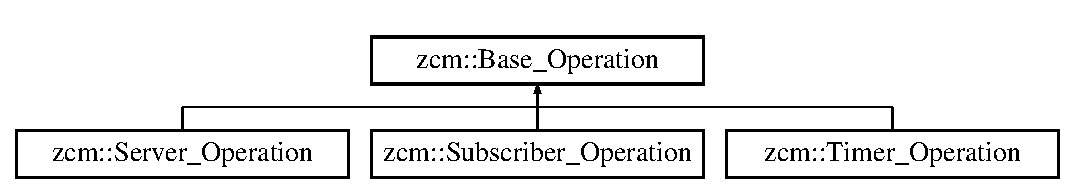
\includegraphics[height=2.000000cm]{classzcm_1_1Base__Operation}
\end{center}
\end{figure}
\subsection*{Public Member Functions}
\begin{DoxyCompactItemize}
\item 
\hyperlink{classzcm_1_1Base__Operation_a87b61a8e801615935c649bae05b9c88e}{Base\-\_\-\-Operation} (std\-::string \hyperlink{classzcm_1_1Base__Operation_a2e2192550818d8f063fc7b2c76c5e21c}{name}, unsigned int \hyperlink{classzcm_1_1Base__Operation_a38af3bcc2578ef215772d595bf3fa358}{priority})
\begin{DoxyCompactList}\small\item\em Construct a base operation. \end{DoxyCompactList}\item 
std\-::string \hyperlink{classzcm_1_1Base__Operation_a46b6a3f23e18bc35425ec2dab80c849f}{get\-\_\-name} ()
\begin{DoxyCompactList}\small\item\em Return the operation name. \end{DoxyCompactList}\item 
unsigned int \hyperlink{classzcm_1_1Base__Operation_a3b15b35c31ed173d2abb193e9fba32ef}{get\-\_\-priority} () const 
\begin{DoxyCompactList}\small\item\em Return the operation priority. \end{DoxyCompactList}\item 
virtual void \hyperlink{classzcm_1_1Base__Operation_a58cb533edd6e6f220d2d1c260fbddca4}{execute} ()
\begin{DoxyCompactList}\small\item\em Virtual execute function overridden by concrete types. \end{DoxyCompactList}\end{DoxyCompactItemize}
\subsection*{Private Attributes}
\begin{DoxyCompactItemize}
\item 
std\-::string \hyperlink{classzcm_1_1Base__Operation_a2e2192550818d8f063fc7b2c76c5e21c}{name}
\begin{DoxyCompactList}\small\item\em Name of the Operation. \end{DoxyCompactList}\item 
unsigned int \hyperlink{classzcm_1_1Base__Operation_a38af3bcc2578ef215772d595bf3fa358}{priority}
\begin{DoxyCompactList}\small\item\em Priority of the Operation. \end{DoxyCompactList}\end{DoxyCompactItemize}


\subsection{Detailed Description}
Base Operation class. 

\subsection{Constructor \& Destructor Documentation}
\hypertarget{classzcm_1_1Base__Operation_a87b61a8e801615935c649bae05b9c88e}{\index{zcm\-::\-Base\-\_\-\-Operation@{zcm\-::\-Base\-\_\-\-Operation}!Base\-\_\-\-Operation@{Base\-\_\-\-Operation}}
\index{Base\-\_\-\-Operation@{Base\-\_\-\-Operation}!zcm::Base_Operation@{zcm\-::\-Base\-\_\-\-Operation}}
\subsubsection[{Base\-\_\-\-Operation}]{\setlength{\rightskip}{0pt plus 5cm}zcm\-::\-Base\-\_\-\-Operation\-::\-Base\-\_\-\-Operation (
\begin{DoxyParamCaption}
\item[{std\-::string}]{name, }
\item[{unsigned int}]{priority}
\end{DoxyParamCaption}
)\hspace{0.3cm}{\ttfamily [inline]}}}\label{classzcm_1_1Base__Operation_a87b61a8e801615935c649bae05b9c88e}


Construct a base operation. 


\begin{DoxyParams}[1]{Parameters}
\mbox{\tt in}  & {\em name} & Name of the operation \\
\hline
\mbox{\tt in}  & {\em priority} & Priority of the operation \\
\hline
\end{DoxyParams}


\subsection{Member Function Documentation}
\hypertarget{classzcm_1_1Base__Operation_a58cb533edd6e6f220d2d1c260fbddca4}{\index{zcm\-::\-Base\-\_\-\-Operation@{zcm\-::\-Base\-\_\-\-Operation}!execute@{execute}}
\index{execute@{execute}!zcm::Base_Operation@{zcm\-::\-Base\-\_\-\-Operation}}
\subsubsection[{execute}]{\setlength{\rightskip}{0pt plus 5cm}virtual void zcm\-::\-Base\-\_\-\-Operation\-::execute (
\begin{DoxyParamCaption}
{}
\end{DoxyParamCaption}
)\hspace{0.3cm}{\ttfamily [inline]}, {\ttfamily [virtual]}}}\label{classzcm_1_1Base__Operation_a58cb533edd6e6f220d2d1c260fbddca4}


Virtual execute function overridden by concrete types. 



Reimplemented in \hyperlink{classzcm_1_1Server__Operation_acd6b89c42aad3df5dc78674770326498}{zcm\-::\-Server\-\_\-\-Operation}, \hyperlink{classzcm_1_1Subscriber__Operation_a2677079c7f3dd85cfc548427c1c101e6}{zcm\-::\-Subscriber\-\_\-\-Operation}, and \hyperlink{classzcm_1_1Timer__Operation_a3693312c4d4d106d0894bb35094efda7}{zcm\-::\-Timer\-\_\-\-Operation}.

\hypertarget{classzcm_1_1Base__Operation_a46b6a3f23e18bc35425ec2dab80c849f}{\index{zcm\-::\-Base\-\_\-\-Operation@{zcm\-::\-Base\-\_\-\-Operation}!get\-\_\-name@{get\-\_\-name}}
\index{get\-\_\-name@{get\-\_\-name}!zcm::Base_Operation@{zcm\-::\-Base\-\_\-\-Operation}}
\subsubsection[{get\-\_\-name}]{\setlength{\rightskip}{0pt plus 5cm}std\-::string zcm\-::\-Base\-\_\-\-Operation\-::get\-\_\-name (
\begin{DoxyParamCaption}
{}
\end{DoxyParamCaption}
)}}\label{classzcm_1_1Base__Operation_a46b6a3f23e18bc35425ec2dab80c849f}


Return the operation name. 

\begin{DoxyReturn}{Returns}
Name of the operation 
\end{DoxyReturn}
\hypertarget{classzcm_1_1Base__Operation_a3b15b35c31ed173d2abb193e9fba32ef}{\index{zcm\-::\-Base\-\_\-\-Operation@{zcm\-::\-Base\-\_\-\-Operation}!get\-\_\-priority@{get\-\_\-priority}}
\index{get\-\_\-priority@{get\-\_\-priority}!zcm::Base_Operation@{zcm\-::\-Base\-\_\-\-Operation}}
\subsubsection[{get\-\_\-priority}]{\setlength{\rightskip}{0pt plus 5cm}unsigned int zcm\-::\-Base\-\_\-\-Operation\-::get\-\_\-priority (
\begin{DoxyParamCaption}
{}
\end{DoxyParamCaption}
) const}}\label{classzcm_1_1Base__Operation_a3b15b35c31ed173d2abb193e9fba32ef}


Return the operation priority. 

\begin{DoxyReturn}{Returns}
Priority of the operation 
\end{DoxyReturn}


\subsection{Member Data Documentation}
\hypertarget{classzcm_1_1Base__Operation_a2e2192550818d8f063fc7b2c76c5e21c}{\index{zcm\-::\-Base\-\_\-\-Operation@{zcm\-::\-Base\-\_\-\-Operation}!name@{name}}
\index{name@{name}!zcm::Base_Operation@{zcm\-::\-Base\-\_\-\-Operation}}
\subsubsection[{name}]{\setlength{\rightskip}{0pt plus 5cm}std\-::string zcm\-::\-Base\-\_\-\-Operation\-::name\hspace{0.3cm}{\ttfamily [private]}}}\label{classzcm_1_1Base__Operation_a2e2192550818d8f063fc7b2c76c5e21c}


Name of the Operation. 

\hypertarget{classzcm_1_1Base__Operation_a38af3bcc2578ef215772d595bf3fa358}{\index{zcm\-::\-Base\-\_\-\-Operation@{zcm\-::\-Base\-\_\-\-Operation}!priority@{priority}}
\index{priority@{priority}!zcm::Base_Operation@{zcm\-::\-Base\-\_\-\-Operation}}
\subsubsection[{priority}]{\setlength{\rightskip}{0pt plus 5cm}unsigned int zcm\-::\-Base\-\_\-\-Operation\-::priority\hspace{0.3cm}{\ttfamily [private]}}}\label{classzcm_1_1Base__Operation_a38af3bcc2578ef215772d595bf3fa358}


Priority of the Operation. 



The documentation for this class was generated from the following files\-:\begin{DoxyCompactItemize}
\item 
/home/kelsier/\-Git\-Hub/zcm/include/\hyperlink{operation__types_8hpp}{operation\-\_\-types.\-hpp}\item 
/home/kelsier/\-Git\-Hub/zcm/src/\hyperlink{operation__types_8cpp}{operation\-\_\-types.\-cpp}\end{DoxyCompactItemize}

\hypertarget{classzcm_1_1Client}{\section{zcm\-:\-:Client Class Reference}
\label{classzcm_1_1Client}\index{zcm\-::\-Client@{zcm\-::\-Client}}
}


\hyperlink{classzcm_1_1Client}{Client} class.  




{\ttfamily \#include $<$client.\-hpp$>$}

\subsection*{Public Member Functions}
\begin{DoxyCompactItemize}
\item 
\hyperlink{classzcm_1_1Client_aeea4b7db3574a527009edc3f41310bcc}{Client} (std\-::string \hyperlink{classzcm_1_1Client_ae972b951134774fd2246d802e2bc6fc0}{name}, zmq\-::context\-\_\-t $\ast$actor\-\_\-context, int timeout)
\begin{DoxyCompactList}\small\item\em Construct a client object. \end{DoxyCompactList}\item 
\hyperlink{classzcm_1_1Client_a6002478c33c7c876de6b1b001121ff87}{Client} (std\-::string \hyperlink{classzcm_1_1Client_ae972b951134774fd2246d802e2bc6fc0}{name}, zmq\-::context\-\_\-t $\ast$actor\-\_\-context, std\-::vector$<$ std\-::string $>$ \hyperlink{classzcm_1_1Client_a01cfee292bb3546a47ec70fff35ff1b6}{endpoints}, int timeout)
\begin{DoxyCompactList}\small\item\em Construct a client object with known endpoints. \end{DoxyCompactList}\item 
\hyperlink{classzcm_1_1Client_a927b35854850369d4d95b3101f3a9baa}{$\sim$\-Client} ()
\begin{DoxyCompactList}\small\item\em Close the client Z\-M\-Q socket and destroy the context. \end{DoxyCompactList}\item 
void \hyperlink{classzcm_1_1Client_aabf03e1bc961b1e525cff57986b1b5a8}{connect} (std\-::vector$<$ std\-::string $>$ new\-\_\-endpoints)
\begin{DoxyCompactList}\small\item\em Connect the client to a new set of endpoints. \end{DoxyCompactList}\item 
std\-::string \hyperlink{classzcm_1_1Client_ad4178e9b209db19994204b9dad7aa374}{get\-\_\-name} ()
\begin{DoxyCompactList}\small\item\em Return the client name. \end{DoxyCompactList}\item 
void \hyperlink{classzcm_1_1Client_aec14e7e61a88c918df8c2bae729923b2}{set\-\_\-timeout} (int timeout)
\begin{DoxyCompactList}\small\item\em Set timeout on the client to prevent endless blocking. \end{DoxyCompactList}\item 
std\-::string \hyperlink{classzcm_1_1Client_a9f62555765181c2feee4631a4b50786d}{call} (std\-::string message)
\begin{DoxyCompactList}\small\item\em Call the server. \end{DoxyCompactList}\end{DoxyCompactItemize}
\subsection*{Private Attributes}
\begin{DoxyCompactItemize}
\item 
std\-::string \hyperlink{classzcm_1_1Client_ae972b951134774fd2246d802e2bc6fc0}{name}
\begin{DoxyCompactList}\small\item\em Name of the publisher. \end{DoxyCompactList}\item 
std\-::vector$<$ std\-::string $>$ \hyperlink{classzcm_1_1Client_a01cfee292bb3546a47ec70fff35ff1b6}{endpoints}
\begin{DoxyCompactList}\small\item\em Vector of endpoints to connect to. \end{DoxyCompactList}\item 
zmq\-::context\-\_\-t $\ast$ \hyperlink{classzcm_1_1Client_a0519b850f2a5167a0636f7a7adcabe1e}{context}
\begin{DoxyCompactList}\small\item\em Z\-M\-Q Context of the client. \end{DoxyCompactList}\item 
zmq\-::socket\-\_\-t $\ast$ \hyperlink{classzcm_1_1Client_a022f5e131d58cea7f6cc49b4580940a0}{client\-\_\-socket}
\begin{DoxyCompactList}\small\item\em Z\-M\-Q Socket of the client. \end{DoxyCompactList}\item 
int \hyperlink{classzcm_1_1Client_a25fa4ff78b8e962ca8436a8815bf7924}{client\-\_\-socket\-\_\-timeout}
\begin{DoxyCompactList}\small\item\em Timeout of the client socket. \end{DoxyCompactList}\end{DoxyCompactItemize}


\subsection{Detailed Description}
\hyperlink{classzcm_1_1Client}{Client} class. 

\subsection{Constructor \& Destructor Documentation}
\hypertarget{classzcm_1_1Client_aeea4b7db3574a527009edc3f41310bcc}{\index{zcm\-::\-Client@{zcm\-::\-Client}!Client@{Client}}
\index{Client@{Client}!zcm::Client@{zcm\-::\-Client}}
\subsubsection[{Client}]{\setlength{\rightskip}{0pt plus 5cm}zcm\-::\-Client\-::\-Client (
\begin{DoxyParamCaption}
\item[{std\-::string}]{name, }
\item[{zmq\-::context\-\_\-t $\ast$}]{actor\-\_\-context, }
\item[{int}]{timeout = {\ttfamily 500}}
\end{DoxyParamCaption}
)}}\label{classzcm_1_1Client_aeea4b7db3574a527009edc3f41310bcc}


Construct a client object. 


\begin{DoxyParams}[1]{Parameters}
\mbox{\tt in}  & {\em name} & \hyperlink{classzcm_1_1Client}{Client} name \\
\hline
\mbox{\tt in}  & {\em Z\-M\-Q} & Context of the \hyperlink{classzcm_1_1Actor}{Actor} Process \\
\hline
\mbox{\tt in}  & {\em timeout} & \hyperlink{classzcm_1_1Client}{Client} socket timeout \\
\hline
\end{DoxyParams}
\hypertarget{classzcm_1_1Client_a6002478c33c7c876de6b1b001121ff87}{\index{zcm\-::\-Client@{zcm\-::\-Client}!Client@{Client}}
\index{Client@{Client}!zcm::Client@{zcm\-::\-Client}}
\subsubsection[{Client}]{\setlength{\rightskip}{0pt plus 5cm}zcm\-::\-Client\-::\-Client (
\begin{DoxyParamCaption}
\item[{std\-::string}]{name, }
\item[{zmq\-::context\-\_\-t $\ast$}]{actor\-\_\-context, }
\item[{std\-::vector$<$ std\-::string $>$}]{endpoints, }
\item[{int}]{timeout = {\ttfamily 500}}
\end{DoxyParamCaption}
)}}\label{classzcm_1_1Client_a6002478c33c7c876de6b1b001121ff87}


Construct a client object with known endpoints. 


\begin{DoxyParams}[1]{Parameters}
\mbox{\tt in}  & {\em name} & \hyperlink{classzcm_1_1Client}{Client} name \\
\hline
\mbox{\tt in}  & {\em Z\-M\-Q} & Context of the \hyperlink{classzcm_1_1Actor}{Actor} Process \\
\hline
\mbox{\tt in}  & {\em endpoints} & A vector of endpoint strings \\
\hline
\mbox{\tt in}  & {\em timeout} & \hyperlink{classzcm_1_1Client}{Client} socket timeout \\
\hline
\end{DoxyParams}
\hypertarget{classzcm_1_1Client_a927b35854850369d4d95b3101f3a9baa}{\index{zcm\-::\-Client@{zcm\-::\-Client}!$\sim$\-Client@{$\sim$\-Client}}
\index{$\sim$\-Client@{$\sim$\-Client}!zcm::Client@{zcm\-::\-Client}}
\subsubsection[{$\sim$\-Client}]{\setlength{\rightskip}{0pt plus 5cm}zcm\-::\-Client\-::$\sim$\-Client (
\begin{DoxyParamCaption}
{}
\end{DoxyParamCaption}
)}}\label{classzcm_1_1Client_a927b35854850369d4d95b3101f3a9baa}


Close the client Z\-M\-Q socket and destroy the context. 



\subsection{Member Function Documentation}
\hypertarget{classzcm_1_1Client_a9f62555765181c2feee4631a4b50786d}{\index{zcm\-::\-Client@{zcm\-::\-Client}!call@{call}}
\index{call@{call}!zcm::Client@{zcm\-::\-Client}}
\subsubsection[{call}]{\setlength{\rightskip}{0pt plus 5cm}std\-::string zcm\-::\-Client\-::call (
\begin{DoxyParamCaption}
\item[{std\-::string}]{message}
\end{DoxyParamCaption}
)}}\label{classzcm_1_1Client_a9f62555765181c2feee4631a4b50786d}


Call the server. 


\begin{DoxyParams}[1]{Parameters}
\mbox{\tt in}  & {\em message} & The message string. Serialize complex objects to strings with protobuf \\
\hline
\end{DoxyParams}
\hypertarget{classzcm_1_1Client_aabf03e1bc961b1e525cff57986b1b5a8}{\index{zcm\-::\-Client@{zcm\-::\-Client}!connect@{connect}}
\index{connect@{connect}!zcm::Client@{zcm\-::\-Client}}
\subsubsection[{connect}]{\setlength{\rightskip}{0pt plus 5cm}void zcm\-::\-Client\-::connect (
\begin{DoxyParamCaption}
\item[{std\-::vector$<$ std\-::string $>$}]{new\-\_\-endpoints}
\end{DoxyParamCaption}
)}}\label{classzcm_1_1Client_aabf03e1bc961b1e525cff57986b1b5a8}


Connect the client to a new set of endpoints. 


\begin{DoxyParams}[1]{Parameters}
\mbox{\tt in}  & {\em new\-\_\-endpoints} & New set of endpoints as a vector \\
\hline
\end{DoxyParams}
\hypertarget{classzcm_1_1Client_ad4178e9b209db19994204b9dad7aa374}{\index{zcm\-::\-Client@{zcm\-::\-Client}!get\-\_\-name@{get\-\_\-name}}
\index{get\-\_\-name@{get\-\_\-name}!zcm::Client@{zcm\-::\-Client}}
\subsubsection[{get\-\_\-name}]{\setlength{\rightskip}{0pt plus 5cm}std\-::string zcm\-::\-Client\-::get\-\_\-name (
\begin{DoxyParamCaption}
{}
\end{DoxyParamCaption}
)}}\label{classzcm_1_1Client_ad4178e9b209db19994204b9dad7aa374}


Return the client name. 

\begin{DoxyReturn}{Returns}
\hyperlink{classzcm_1_1Client}{Client} name 
\end{DoxyReturn}
\hypertarget{classzcm_1_1Client_aec14e7e61a88c918df8c2bae729923b2}{\index{zcm\-::\-Client@{zcm\-::\-Client}!set\-\_\-timeout@{set\-\_\-timeout}}
\index{set\-\_\-timeout@{set\-\_\-timeout}!zcm::Client@{zcm\-::\-Client}}
\subsubsection[{set\-\_\-timeout}]{\setlength{\rightskip}{0pt plus 5cm}void zcm\-::\-Client\-::set\-\_\-timeout (
\begin{DoxyParamCaption}
\item[{int}]{timeout}
\end{DoxyParamCaption}
)}}\label{classzcm_1_1Client_aec14e7e61a88c918df8c2bae729923b2}


Set timeout on the client to prevent endless blocking. 


\begin{DoxyParams}[1]{Parameters}
\mbox{\tt in}  & {\em timeout} & New timeout value \\
\hline
\end{DoxyParams}


\subsection{Member Data Documentation}
\hypertarget{classzcm_1_1Client_a022f5e131d58cea7f6cc49b4580940a0}{\index{zcm\-::\-Client@{zcm\-::\-Client}!client\-\_\-socket@{client\-\_\-socket}}
\index{client\-\_\-socket@{client\-\_\-socket}!zcm::Client@{zcm\-::\-Client}}
\subsubsection[{client\-\_\-socket}]{\setlength{\rightskip}{0pt plus 5cm}zmq\-::socket\-\_\-t$\ast$ zcm\-::\-Client\-::client\-\_\-socket\hspace{0.3cm}{\ttfamily [private]}}}\label{classzcm_1_1Client_a022f5e131d58cea7f6cc49b4580940a0}


Z\-M\-Q Socket of the client. 

\hypertarget{classzcm_1_1Client_a25fa4ff78b8e962ca8436a8815bf7924}{\index{zcm\-::\-Client@{zcm\-::\-Client}!client\-\_\-socket\-\_\-timeout@{client\-\_\-socket\-\_\-timeout}}
\index{client\-\_\-socket\-\_\-timeout@{client\-\_\-socket\-\_\-timeout}!zcm::Client@{zcm\-::\-Client}}
\subsubsection[{client\-\_\-socket\-\_\-timeout}]{\setlength{\rightskip}{0pt plus 5cm}int zcm\-::\-Client\-::client\-\_\-socket\-\_\-timeout\hspace{0.3cm}{\ttfamily [private]}}}\label{classzcm_1_1Client_a25fa4ff78b8e962ca8436a8815bf7924}


Timeout of the client socket. 

\hypertarget{classzcm_1_1Client_a0519b850f2a5167a0636f7a7adcabe1e}{\index{zcm\-::\-Client@{zcm\-::\-Client}!context@{context}}
\index{context@{context}!zcm::Client@{zcm\-::\-Client}}
\subsubsection[{context}]{\setlength{\rightskip}{0pt plus 5cm}zmq\-::context\-\_\-t$\ast$ zcm\-::\-Client\-::context\hspace{0.3cm}{\ttfamily [private]}}}\label{classzcm_1_1Client_a0519b850f2a5167a0636f7a7adcabe1e}


Z\-M\-Q Context of the client. 

\hypertarget{classzcm_1_1Client_a01cfee292bb3546a47ec70fff35ff1b6}{\index{zcm\-::\-Client@{zcm\-::\-Client}!endpoints@{endpoints}}
\index{endpoints@{endpoints}!zcm::Client@{zcm\-::\-Client}}
\subsubsection[{endpoints}]{\setlength{\rightskip}{0pt plus 5cm}std\-::vector$<$std\-::string$>$ zcm\-::\-Client\-::endpoints\hspace{0.3cm}{\ttfamily [private]}}}\label{classzcm_1_1Client_a01cfee292bb3546a47ec70fff35ff1b6}


Vector of endpoints to connect to. 

\hypertarget{classzcm_1_1Client_ae972b951134774fd2246d802e2bc6fc0}{\index{zcm\-::\-Client@{zcm\-::\-Client}!name@{name}}
\index{name@{name}!zcm::Client@{zcm\-::\-Client}}
\subsubsection[{name}]{\setlength{\rightskip}{0pt plus 5cm}std\-::string zcm\-::\-Client\-::name\hspace{0.3cm}{\ttfamily [private]}}}\label{classzcm_1_1Client_ae972b951134774fd2246d802e2bc6fc0}


Name of the publisher. 



The documentation for this class was generated from the following files\-:\begin{DoxyCompactItemize}
\item 
/home/kelsier/\-Git\-Hub/zcm/include/\hyperlink{client_8hpp}{client.\-hpp}\item 
/home/kelsier/\-Git\-Hub/zcm/src/\hyperlink{client_8cpp}{client.\-cpp}\end{DoxyCompactItemize}

\hypertarget{classzcm_1_1Component}{}\section{zcm\+:\+:Component Class Reference}
\label{classzcm_1_1Component}\index{zcm\+::\+Component@{zcm\+::\+Component}}


\hyperlink{classzcm_1_1Component}{Component} class.  




{\ttfamily \#include $<$component.\+hpp$>$}

\subsection*{Public Member Functions}
\begin{DoxyCompactItemize}
\item 
\hyperlink{classzcm_1_1Component_a6fd6b1f309a6b464a14c22a94d18f040}{Component} ()
\begin{DoxyCompactList}\small\item\em Construct a component Prepare the component operation queue. \end{DoxyCompactList}\item 
\hyperlink{classzcm_1_1Component_a0bab6bb89e49affa281179f5d6aeff6a}{$\sim$\+Component} ()
\begin{DoxyCompactList}\small\item\em Destroy the component. \end{DoxyCompactList}\item 
\hyperlink{classzcm_1_1Timer}{Timer} $\ast$ \hyperlink{classzcm_1_1Component_a9fe1a846945403f152e069917f2f49b2}{get\+\_\+timer} (std\+::string timer\+\_\+name)
\begin{DoxyCompactList}\small\item\em Get a component timer by name. \end{DoxyCompactList}\item 
\hyperlink{classzcm_1_1Publisher}{Publisher} $\ast$ \hyperlink{classzcm_1_1Component_a9bbbc50ea3f1a278bf74848f784df493}{get\+\_\+publisher} (std\+::string publisher\+\_\+name)
\begin{DoxyCompactList}\small\item\em Get a component publisher by name. \end{DoxyCompactList}\item 
\hyperlink{classzcm_1_1Subscriber}{Subscriber} $\ast$ \hyperlink{classzcm_1_1Component_a4865551765c7d0ead713ad65571aa8dc}{get\+\_\+subscriber} (std\+::string subscriber\+\_\+name)
\begin{DoxyCompactList}\small\item\em Get a component subscriber by name. \end{DoxyCompactList}\item 
\hyperlink{classzcm_1_1Client}{Client} $\ast$ \hyperlink{classzcm_1_1Component_a89e3f610505b007767f10235b4ea8c20}{get\+\_\+client} (std\+::string client\+\_\+name)
\begin{DoxyCompactList}\small\item\em Get a component client by name. \end{DoxyCompactList}\item 
\hyperlink{classzcm_1_1Server}{Server} $\ast$ \hyperlink{classzcm_1_1Component_a80e221012442119feb53740510242117}{get\+\_\+server} (std\+::string server\+\_\+name)
\begin{DoxyCompactList}\small\item\em Get a component server by name. \end{DoxyCompactList}\item 
void \hyperlink{classzcm_1_1Component_ac9b656236674930c58f7dbfebb063da9}{add\+\_\+timer} (\hyperlink{classzcm_1_1Timer}{Timer} $\ast$new\+\_\+timer)
\begin{DoxyCompactList}\small\item\em Add a timer to this component. \end{DoxyCompactList}\item 
void \hyperlink{classzcm_1_1Component_a3d70420843fc7e0ff2d3d2edc422e992}{add\+\_\+publisher} (\hyperlink{classzcm_1_1Publisher}{Publisher} $\ast$new\+\_\+publisher)
\begin{DoxyCompactList}\small\item\em Add a publisher to this component. \end{DoxyCompactList}\item 
void \hyperlink{classzcm_1_1Component_ac07614093c36e61704d166f00f14c22e}{add\+\_\+subscriber} (\hyperlink{classzcm_1_1Subscriber}{Subscriber} $\ast$new\+\_\+subscriber)
\begin{DoxyCompactList}\small\item\em Add a subscriber to this component. \end{DoxyCompactList}\item 
void \hyperlink{classzcm_1_1Component_ad71bf4cebc218089642d16f697a493fa}{add\+\_\+client} (\hyperlink{classzcm_1_1Client}{Client} $\ast$new\+\_\+client)
\begin{DoxyCompactList}\small\item\em Add a client to this component. \end{DoxyCompactList}\item 
void \hyperlink{classzcm_1_1Component_a31989e75d9de6093cb712148cd94da71}{add\+\_\+server} (\hyperlink{classzcm_1_1Server}{Server} $\ast$new\+\_\+server)
\begin{DoxyCompactList}\small\item\em Add a server to this component. \end{DoxyCompactList}\item 
void \hyperlink{classzcm_1_1Component_a64674700fb1edd7c84a64ce78aa5b2f4}{configure\+\_\+publishers} (std\+::map$<$ std\+::string, std\+::vector$<$ std\+::string $>$$>$ publisher\+\_\+endpoints)
\begin{DoxyCompactList}\small\item\em Configure all component publishers. \end{DoxyCompactList}\item 
void \hyperlink{classzcm_1_1Component_a25c31193982bb317186f4f3b4d8d790c}{configure\+\_\+subscribers} (std\+::map$<$ std\+::string, std\+::vector$<$ std\+::string $>$$>$ subscriber\+\_\+endpoints)
\begin{DoxyCompactList}\small\item\em Configure all component subscribers. \end{DoxyCompactList}\item 
void \hyperlink{classzcm_1_1Component_ad3ed49fb7e936de3fd66ac4e37974735}{configure\+\_\+clients} (std\+::map$<$ std\+::string, std\+::vector$<$ std\+::string $>$$>$ client\+\_\+endpoints)
\begin{DoxyCompactList}\small\item\em Configure all component clients. \end{DoxyCompactList}\item 
void \hyperlink{classzcm_1_1Component_a9a8df5c1a899ec4470dd5bbcd90e9e79}{configure\+\_\+servers} (std\+::map$<$ std\+::string, std\+::vector$<$ std\+::string $>$$>$ server\+\_\+endpoints)
\begin{DoxyCompactList}\small\item\em Configure all component servers. \end{DoxyCompactList}\item 
std\+::thread $\ast$ \hyperlink{classzcm_1_1Component_a328d6f79aab5455e96a2badfdb6bb451}{spawn} ()
\begin{DoxyCompactList}\small\item\em Spawn the component executor thread. \end{DoxyCompactList}\end{DoxyCompactItemize}
\subsection*{Protected Attributes}
\begin{DoxyCompactItemize}
\item 
\hyperlink{classzcm_1_1Operation__Queue}{Operation\+\_\+\+Queue} $\ast$ \hyperlink{classzcm_1_1Component_a4c9f3591c18dde89bc3c2af7717c6692}{operation\+\_\+queue}
\begin{DoxyCompactList}\small\item\em Pointer to the \hyperlink{classzcm_1_1Component}{Component} Operation Queue. \end{DoxyCompactList}\item 
std\+::thread $\ast$ \hyperlink{classzcm_1_1Component_a392ca3b6cd537cd7aa1d4db31dacdf4d}{executor\+\_\+thread}
\begin{DoxyCompactList}\small\item\em Pointer to the \hyperlink{classzcm_1_1Component}{Component} Executor Thread. \end{DoxyCompactList}\item 
std\+::vector$<$ \hyperlink{classzcm_1_1Timer}{Timer} $\ast$ $>$ \hyperlink{classzcm_1_1Component_a506eac4aebc9e02f0df246afbbac7d75}{timers}
\begin{DoxyCompactList}\small\item\em A vector of component timers. \end{DoxyCompactList}\item 
std\+::vector$<$ \hyperlink{classzcm_1_1Publisher}{Publisher} $\ast$ $>$ \hyperlink{classzcm_1_1Component_a4dcce63b0b5495bc15bd18e5dce86094}{publishers}
\begin{DoxyCompactList}\small\item\em A vector of component publishers. \end{DoxyCompactList}\item 
std\+::vector$<$ \hyperlink{classzcm_1_1Subscriber}{Subscriber} $\ast$ $>$ \hyperlink{classzcm_1_1Component_a9f9e58fb5d2189b183ffd22ce905d620}{subscribers}
\begin{DoxyCompactList}\small\item\em A vector of component subscribers. \end{DoxyCompactList}\item 
std\+::vector$<$ \hyperlink{classzcm_1_1Client}{Client} $\ast$ $>$ \hyperlink{classzcm_1_1Component_a940e1b9755cd9f2bea95bda880999626}{clients}
\begin{DoxyCompactList}\small\item\em A vector of component clients. \end{DoxyCompactList}\item 
std\+::vector$<$ \hyperlink{classzcm_1_1Server}{Server} $\ast$ $>$ \hyperlink{classzcm_1_1Component_a1d99508f165f7014b190d2fbe4ad2271}{servers}
\begin{DoxyCompactList}\small\item\em A vector of component servers. \end{DoxyCompactList}\end{DoxyCompactItemize}


\subsection{Detailed Description}
\hyperlink{classzcm_1_1Component}{Component} class. 

\subsection{Constructor \& Destructor Documentation}
\index{zcm\+::\+Component@{zcm\+::\+Component}!Component@{Component}}
\index{Component@{Component}!zcm\+::\+Component@{zcm\+::\+Component}}
\subsubsection[{\texorpdfstring{Component()}{Component()}}]{\setlength{\rightskip}{0pt plus 5cm}zcm\+::\+Component\+::\+Component (
\begin{DoxyParamCaption}
{}
\end{DoxyParamCaption}
)}\hypertarget{classzcm_1_1Component_a6fd6b1f309a6b464a14c22a94d18f040}{}\label{classzcm_1_1Component_a6fd6b1f309a6b464a14c22a94d18f040}


Construct a component Prepare the component operation queue. 

\index{zcm\+::\+Component@{zcm\+::\+Component}!````~Component@{$\sim$\+Component}}
\index{````~Component@{$\sim$\+Component}!zcm\+::\+Component@{zcm\+::\+Component}}
\subsubsection[{\texorpdfstring{$\sim$\+Component()}{~Component()}}]{\setlength{\rightskip}{0pt plus 5cm}zcm\+::\+Component\+::$\sim$\+Component (
\begin{DoxyParamCaption}
{}
\end{DoxyParamCaption}
)}\hypertarget{classzcm_1_1Component_a0bab6bb89e49affa281179f5d6aeff6a}{}\label{classzcm_1_1Component_a0bab6bb89e49affa281179f5d6aeff6a}


Destroy the component. 



\subsection{Member Function Documentation}
\index{zcm\+::\+Component@{zcm\+::\+Component}!add\+\_\+client@{add\+\_\+client}}
\index{add\+\_\+client@{add\+\_\+client}!zcm\+::\+Component@{zcm\+::\+Component}}
\subsubsection[{\texorpdfstring{add\+\_\+client(\+Client $\ast$new\+\_\+client)}{add_client(Client *new_client)}}]{\setlength{\rightskip}{0pt plus 5cm}void zcm\+::\+Component\+::add\+\_\+client (
\begin{DoxyParamCaption}
\item[{{\bf Client} $\ast$}]{new\+\_\+client}
\end{DoxyParamCaption}
)}\hypertarget{classzcm_1_1Component_ad71bf4cebc218089642d16f697a493fa}{}\label{classzcm_1_1Component_ad71bf4cebc218089642d16f697a493fa}


Add a client to this component. 


\begin{DoxyParams}[1]{Parameters}
\mbox{\tt in}  & {\em new\+\_\+client} & Pointer to a client object \\
\hline
\end{DoxyParams}
\index{zcm\+::\+Component@{zcm\+::\+Component}!add\+\_\+publisher@{add\+\_\+publisher}}
\index{add\+\_\+publisher@{add\+\_\+publisher}!zcm\+::\+Component@{zcm\+::\+Component}}
\subsubsection[{\texorpdfstring{add\+\_\+publisher(\+Publisher $\ast$new\+\_\+publisher)}{add_publisher(Publisher *new_publisher)}}]{\setlength{\rightskip}{0pt plus 5cm}void zcm\+::\+Component\+::add\+\_\+publisher (
\begin{DoxyParamCaption}
\item[{{\bf Publisher} $\ast$}]{new\+\_\+publisher}
\end{DoxyParamCaption}
)}\hypertarget{classzcm_1_1Component_a3d70420843fc7e0ff2d3d2edc422e992}{}\label{classzcm_1_1Component_a3d70420843fc7e0ff2d3d2edc422e992}


Add a publisher to this component. 


\begin{DoxyParams}[1]{Parameters}
\mbox{\tt in}  & {\em new\+\_\+publisher} & Pointer to a publisher object \\
\hline
\end{DoxyParams}
\index{zcm\+::\+Component@{zcm\+::\+Component}!add\+\_\+server@{add\+\_\+server}}
\index{add\+\_\+server@{add\+\_\+server}!zcm\+::\+Component@{zcm\+::\+Component}}
\subsubsection[{\texorpdfstring{add\+\_\+server(\+Server $\ast$new\+\_\+server)}{add_server(Server *new_server)}}]{\setlength{\rightskip}{0pt plus 5cm}void zcm\+::\+Component\+::add\+\_\+server (
\begin{DoxyParamCaption}
\item[{{\bf Server} $\ast$}]{new\+\_\+server}
\end{DoxyParamCaption}
)}\hypertarget{classzcm_1_1Component_a31989e75d9de6093cb712148cd94da71}{}\label{classzcm_1_1Component_a31989e75d9de6093cb712148cd94da71}


Add a server to this component. 


\begin{DoxyParams}[1]{Parameters}
\mbox{\tt in}  & {\em new\+\_\+server} & Pointer to a server object \\
\hline
\end{DoxyParams}
\index{zcm\+::\+Component@{zcm\+::\+Component}!add\+\_\+subscriber@{add\+\_\+subscriber}}
\index{add\+\_\+subscriber@{add\+\_\+subscriber}!zcm\+::\+Component@{zcm\+::\+Component}}
\subsubsection[{\texorpdfstring{add\+\_\+subscriber(\+Subscriber $\ast$new\+\_\+subscriber)}{add_subscriber(Subscriber *new_subscriber)}}]{\setlength{\rightskip}{0pt plus 5cm}void zcm\+::\+Component\+::add\+\_\+subscriber (
\begin{DoxyParamCaption}
\item[{{\bf Subscriber} $\ast$}]{new\+\_\+subscriber}
\end{DoxyParamCaption}
)}\hypertarget{classzcm_1_1Component_ac07614093c36e61704d166f00f14c22e}{}\label{classzcm_1_1Component_ac07614093c36e61704d166f00f14c22e}


Add a subscriber to this component. 


\begin{DoxyParams}[1]{Parameters}
\mbox{\tt in}  & {\em new\+\_\+subscriber} & Pointer to a subscriber object \\
\hline
\end{DoxyParams}
\index{zcm\+::\+Component@{zcm\+::\+Component}!add\+\_\+timer@{add\+\_\+timer}}
\index{add\+\_\+timer@{add\+\_\+timer}!zcm\+::\+Component@{zcm\+::\+Component}}
\subsubsection[{\texorpdfstring{add\+\_\+timer(\+Timer $\ast$new\+\_\+timer)}{add_timer(Timer *new_timer)}}]{\setlength{\rightskip}{0pt plus 5cm}void zcm\+::\+Component\+::add\+\_\+timer (
\begin{DoxyParamCaption}
\item[{{\bf Timer} $\ast$}]{new\+\_\+timer}
\end{DoxyParamCaption}
)}\hypertarget{classzcm_1_1Component_ac9b656236674930c58f7dbfebb063da9}{}\label{classzcm_1_1Component_ac9b656236674930c58f7dbfebb063da9}


Add a timer to this component. 


\begin{DoxyParams}[1]{Parameters}
\mbox{\tt in}  & {\em new\+\_\+timer} & Pointer to a timer object \\
\hline
\end{DoxyParams}
\index{zcm\+::\+Component@{zcm\+::\+Component}!configure\+\_\+clients@{configure\+\_\+clients}}
\index{configure\+\_\+clients@{configure\+\_\+clients}!zcm\+::\+Component@{zcm\+::\+Component}}
\subsubsection[{\texorpdfstring{configure\+\_\+clients(std\+::map$<$ std\+::string, std\+::vector$<$ std\+::string $>$$>$ client\+\_\+endpoints)}{configure_clients(std::map< std::string, std::vector< std::string >> client_endpoints)}}]{\setlength{\rightskip}{0pt plus 5cm}void zcm\+::\+Component\+::configure\+\_\+clients (
\begin{DoxyParamCaption}
\item[{std\+::map$<$ std\+::string, std\+::vector$<$ std\+::string $>$$>$}]{client\+\_\+endpoints}
\end{DoxyParamCaption}
)}\hypertarget{classzcm_1_1Component_ad3ed49fb7e936de3fd66ac4e37974735}{}\label{classzcm_1_1Component_ad3ed49fb7e936de3fd66ac4e37974735}


Configure all component clients. 


\begin{DoxyParams}[1]{Parameters}
\mbox{\tt in}  & {\em client\+\_\+endpoints} & A map of endpoints for all clients \\
\hline
\end{DoxyParams}
\index{zcm\+::\+Component@{zcm\+::\+Component}!configure\+\_\+publishers@{configure\+\_\+publishers}}
\index{configure\+\_\+publishers@{configure\+\_\+publishers}!zcm\+::\+Component@{zcm\+::\+Component}}
\subsubsection[{\texorpdfstring{configure\+\_\+publishers(std\+::map$<$ std\+::string, std\+::vector$<$ std\+::string $>$$>$ publisher\+\_\+endpoints)}{configure_publishers(std::map< std::string, std::vector< std::string >> publisher_endpoints)}}]{\setlength{\rightskip}{0pt plus 5cm}void zcm\+::\+Component\+::configure\+\_\+publishers (
\begin{DoxyParamCaption}
\item[{std\+::map$<$ std\+::string, std\+::vector$<$ std\+::string $>$$>$}]{publisher\+\_\+endpoints}
\end{DoxyParamCaption}
)}\hypertarget{classzcm_1_1Component_a64674700fb1edd7c84a64ce78aa5b2f4}{}\label{classzcm_1_1Component_a64674700fb1edd7c84a64ce78aa5b2f4}


Configure all component publishers. 


\begin{DoxyParams}[1]{Parameters}
\mbox{\tt in}  & {\em publisher\+\_\+endpoints} & A map of endpoints for all publishers \\
\hline
\end{DoxyParams}
\index{zcm\+::\+Component@{zcm\+::\+Component}!configure\+\_\+servers@{configure\+\_\+servers}}
\index{configure\+\_\+servers@{configure\+\_\+servers}!zcm\+::\+Component@{zcm\+::\+Component}}
\subsubsection[{\texorpdfstring{configure\+\_\+servers(std\+::map$<$ std\+::string, std\+::vector$<$ std\+::string $>$$>$ server\+\_\+endpoints)}{configure_servers(std::map< std::string, std::vector< std::string >> server_endpoints)}}]{\setlength{\rightskip}{0pt plus 5cm}void zcm\+::\+Component\+::configure\+\_\+servers (
\begin{DoxyParamCaption}
\item[{std\+::map$<$ std\+::string, std\+::vector$<$ std\+::string $>$$>$}]{server\+\_\+endpoints}
\end{DoxyParamCaption}
)}\hypertarget{classzcm_1_1Component_a9a8df5c1a899ec4470dd5bbcd90e9e79}{}\label{classzcm_1_1Component_a9a8df5c1a899ec4470dd5bbcd90e9e79}


Configure all component servers. 


\begin{DoxyParams}[1]{Parameters}
\mbox{\tt in}  & {\em server\+\_\+endpoints} & A map of endpoints for all servers \\
\hline
\end{DoxyParams}
\index{zcm\+::\+Component@{zcm\+::\+Component}!configure\+\_\+subscribers@{configure\+\_\+subscribers}}
\index{configure\+\_\+subscribers@{configure\+\_\+subscribers}!zcm\+::\+Component@{zcm\+::\+Component}}
\subsubsection[{\texorpdfstring{configure\+\_\+subscribers(std\+::map$<$ std\+::string, std\+::vector$<$ std\+::string $>$$>$ subscriber\+\_\+endpoints)}{configure_subscribers(std::map< std::string, std::vector< std::string >> subscriber_endpoints)}}]{\setlength{\rightskip}{0pt plus 5cm}void zcm\+::\+Component\+::configure\+\_\+subscribers (
\begin{DoxyParamCaption}
\item[{std\+::map$<$ std\+::string, std\+::vector$<$ std\+::string $>$$>$}]{subscriber\+\_\+endpoints}
\end{DoxyParamCaption}
)}\hypertarget{classzcm_1_1Component_a25c31193982bb317186f4f3b4d8d790c}{}\label{classzcm_1_1Component_a25c31193982bb317186f4f3b4d8d790c}


Configure all component subscribers. 


\begin{DoxyParams}[1]{Parameters}
\mbox{\tt in}  & {\em subscriber\+\_\+endpoints} & A map of endpoints for all subscribers \\
\hline
\end{DoxyParams}
\index{zcm\+::\+Component@{zcm\+::\+Component}!get\+\_\+client@{get\+\_\+client}}
\index{get\+\_\+client@{get\+\_\+client}!zcm\+::\+Component@{zcm\+::\+Component}}
\subsubsection[{\texorpdfstring{get\+\_\+client(std\+::string client\+\_\+name)}{get_client(std::string client_name)}}]{\setlength{\rightskip}{0pt plus 5cm}{\bf Client} $\ast$ zcm\+::\+Component\+::get\+\_\+client (
\begin{DoxyParamCaption}
\item[{std\+::string}]{client\+\_\+name}
\end{DoxyParamCaption}
)}\hypertarget{classzcm_1_1Component_a89e3f610505b007767f10235b4ea8c20}{}\label{classzcm_1_1Component_a89e3f610505b007767f10235b4ea8c20}


Get a component client by name. 


\begin{DoxyParams}[1]{Parameters}
\mbox{\tt in}  & {\em client\+\_\+name} & Name of the client \\
\hline
\end{DoxyParams}
\index{zcm\+::\+Component@{zcm\+::\+Component}!get\+\_\+publisher@{get\+\_\+publisher}}
\index{get\+\_\+publisher@{get\+\_\+publisher}!zcm\+::\+Component@{zcm\+::\+Component}}
\subsubsection[{\texorpdfstring{get\+\_\+publisher(std\+::string publisher\+\_\+name)}{get_publisher(std::string publisher_name)}}]{\setlength{\rightskip}{0pt plus 5cm}{\bf Publisher} $\ast$ zcm\+::\+Component\+::get\+\_\+publisher (
\begin{DoxyParamCaption}
\item[{std\+::string}]{publisher\+\_\+name}
\end{DoxyParamCaption}
)}\hypertarget{classzcm_1_1Component_a9bbbc50ea3f1a278bf74848f784df493}{}\label{classzcm_1_1Component_a9bbbc50ea3f1a278bf74848f784df493}


Get a component publisher by name. 


\begin{DoxyParams}[1]{Parameters}
\mbox{\tt in}  & {\em publisher\+\_\+name} & Name of the publisher \\
\hline
\end{DoxyParams}
\index{zcm\+::\+Component@{zcm\+::\+Component}!get\+\_\+server@{get\+\_\+server}}
\index{get\+\_\+server@{get\+\_\+server}!zcm\+::\+Component@{zcm\+::\+Component}}
\subsubsection[{\texorpdfstring{get\+\_\+server(std\+::string server\+\_\+name)}{get_server(std::string server_name)}}]{\setlength{\rightskip}{0pt plus 5cm}{\bf Server} $\ast$ zcm\+::\+Component\+::get\+\_\+server (
\begin{DoxyParamCaption}
\item[{std\+::string}]{server\+\_\+name}
\end{DoxyParamCaption}
)}\hypertarget{classzcm_1_1Component_a80e221012442119feb53740510242117}{}\label{classzcm_1_1Component_a80e221012442119feb53740510242117}


Get a component server by name. 


\begin{DoxyParams}[1]{Parameters}
\mbox{\tt in}  & {\em server\+\_\+name} & Name of the server \\
\hline
\end{DoxyParams}
\index{zcm\+::\+Component@{zcm\+::\+Component}!get\+\_\+subscriber@{get\+\_\+subscriber}}
\index{get\+\_\+subscriber@{get\+\_\+subscriber}!zcm\+::\+Component@{zcm\+::\+Component}}
\subsubsection[{\texorpdfstring{get\+\_\+subscriber(std\+::string subscriber\+\_\+name)}{get_subscriber(std::string subscriber_name)}}]{\setlength{\rightskip}{0pt plus 5cm}{\bf Subscriber} $\ast$ zcm\+::\+Component\+::get\+\_\+subscriber (
\begin{DoxyParamCaption}
\item[{std\+::string}]{subscriber\+\_\+name}
\end{DoxyParamCaption}
)}\hypertarget{classzcm_1_1Component_a4865551765c7d0ead713ad65571aa8dc}{}\label{classzcm_1_1Component_a4865551765c7d0ead713ad65571aa8dc}


Get a component subscriber by name. 


\begin{DoxyParams}[1]{Parameters}
\mbox{\tt in}  & {\em subscriber\+\_\+name} & Name of the subscriber \\
\hline
\end{DoxyParams}
\index{zcm\+::\+Component@{zcm\+::\+Component}!get\+\_\+timer@{get\+\_\+timer}}
\index{get\+\_\+timer@{get\+\_\+timer}!zcm\+::\+Component@{zcm\+::\+Component}}
\subsubsection[{\texorpdfstring{get\+\_\+timer(std\+::string timer\+\_\+name)}{get_timer(std::string timer_name)}}]{\setlength{\rightskip}{0pt plus 5cm}{\bf Timer} $\ast$ zcm\+::\+Component\+::get\+\_\+timer (
\begin{DoxyParamCaption}
\item[{std\+::string}]{timer\+\_\+name}
\end{DoxyParamCaption}
)}\hypertarget{classzcm_1_1Component_a9fe1a846945403f152e069917f2f49b2}{}\label{classzcm_1_1Component_a9fe1a846945403f152e069917f2f49b2}


Get a component timer by name. 


\begin{DoxyParams}[1]{Parameters}
\mbox{\tt in}  & {\em timer\+\_\+name} & Name of the timer \\
\hline
\end{DoxyParams}
\index{zcm\+::\+Component@{zcm\+::\+Component}!spawn@{spawn}}
\index{spawn@{spawn}!zcm\+::\+Component@{zcm\+::\+Component}}
\subsubsection[{\texorpdfstring{spawn()}{spawn()}}]{\setlength{\rightskip}{0pt plus 5cm}std\+::thread $\ast$ zcm\+::\+Component\+::spawn (
\begin{DoxyParamCaption}
{}
\end{DoxyParamCaption}
)}\hypertarget{classzcm_1_1Component_a328d6f79aab5455e96a2badfdb6bb451}{}\label{classzcm_1_1Component_a328d6f79aab5455e96a2badfdb6bb451}


Spawn the component executor thread. 

\begin{DoxyReturn}{Returns}
Return a pointer to the executor thread 
\end{DoxyReturn}


\subsection{Member Data Documentation}
\index{zcm\+::\+Component@{zcm\+::\+Component}!clients@{clients}}
\index{clients@{clients}!zcm\+::\+Component@{zcm\+::\+Component}}
\subsubsection[{\texorpdfstring{clients}{clients}}]{\setlength{\rightskip}{0pt plus 5cm}std\+::vector$<${\bf Client}$\ast$$>$ zcm\+::\+Component\+::clients\hspace{0.3cm}{\ttfamily [protected]}}\hypertarget{classzcm_1_1Component_a940e1b9755cd9f2bea95bda880999626}{}\label{classzcm_1_1Component_a940e1b9755cd9f2bea95bda880999626}


A vector of component clients. 

\index{zcm\+::\+Component@{zcm\+::\+Component}!executor\+\_\+thread@{executor\+\_\+thread}}
\index{executor\+\_\+thread@{executor\+\_\+thread}!zcm\+::\+Component@{zcm\+::\+Component}}
\subsubsection[{\texorpdfstring{executor\+\_\+thread}{executor_thread}}]{\setlength{\rightskip}{0pt plus 5cm}std\+::thread$\ast$ zcm\+::\+Component\+::executor\+\_\+thread\hspace{0.3cm}{\ttfamily [protected]}}\hypertarget{classzcm_1_1Component_a392ca3b6cd537cd7aa1d4db31dacdf4d}{}\label{classzcm_1_1Component_a392ca3b6cd537cd7aa1d4db31dacdf4d}


Pointer to the \hyperlink{classzcm_1_1Component}{Component} Executor Thread. 

\index{zcm\+::\+Component@{zcm\+::\+Component}!operation\+\_\+queue@{operation\+\_\+queue}}
\index{operation\+\_\+queue@{operation\+\_\+queue}!zcm\+::\+Component@{zcm\+::\+Component}}
\subsubsection[{\texorpdfstring{operation\+\_\+queue}{operation_queue}}]{\setlength{\rightskip}{0pt plus 5cm}{\bf Operation\+\_\+\+Queue}$\ast$ zcm\+::\+Component\+::operation\+\_\+queue\hspace{0.3cm}{\ttfamily [protected]}}\hypertarget{classzcm_1_1Component_a4c9f3591c18dde89bc3c2af7717c6692}{}\label{classzcm_1_1Component_a4c9f3591c18dde89bc3c2af7717c6692}


Pointer to the \hyperlink{classzcm_1_1Component}{Component} Operation Queue. 

\index{zcm\+::\+Component@{zcm\+::\+Component}!publishers@{publishers}}
\index{publishers@{publishers}!zcm\+::\+Component@{zcm\+::\+Component}}
\subsubsection[{\texorpdfstring{publishers}{publishers}}]{\setlength{\rightskip}{0pt plus 5cm}std\+::vector$<${\bf Publisher}$\ast$$>$ zcm\+::\+Component\+::publishers\hspace{0.3cm}{\ttfamily [protected]}}\hypertarget{classzcm_1_1Component_a4dcce63b0b5495bc15bd18e5dce86094}{}\label{classzcm_1_1Component_a4dcce63b0b5495bc15bd18e5dce86094}


A vector of component publishers. 

\index{zcm\+::\+Component@{zcm\+::\+Component}!servers@{servers}}
\index{servers@{servers}!zcm\+::\+Component@{zcm\+::\+Component}}
\subsubsection[{\texorpdfstring{servers}{servers}}]{\setlength{\rightskip}{0pt plus 5cm}std\+::vector$<${\bf Server}$\ast$$>$ zcm\+::\+Component\+::servers\hspace{0.3cm}{\ttfamily [protected]}}\hypertarget{classzcm_1_1Component_a1d99508f165f7014b190d2fbe4ad2271}{}\label{classzcm_1_1Component_a1d99508f165f7014b190d2fbe4ad2271}


A vector of component servers. 

\index{zcm\+::\+Component@{zcm\+::\+Component}!subscribers@{subscribers}}
\index{subscribers@{subscribers}!zcm\+::\+Component@{zcm\+::\+Component}}
\subsubsection[{\texorpdfstring{subscribers}{subscribers}}]{\setlength{\rightskip}{0pt plus 5cm}std\+::vector$<${\bf Subscriber}$\ast$$>$ zcm\+::\+Component\+::subscribers\hspace{0.3cm}{\ttfamily [protected]}}\hypertarget{classzcm_1_1Component_a9f9e58fb5d2189b183ffd22ce905d620}{}\label{classzcm_1_1Component_a9f9e58fb5d2189b183ffd22ce905d620}


A vector of component subscribers. 

\index{zcm\+::\+Component@{zcm\+::\+Component}!timers@{timers}}
\index{timers@{timers}!zcm\+::\+Component@{zcm\+::\+Component}}
\subsubsection[{\texorpdfstring{timers}{timers}}]{\setlength{\rightskip}{0pt plus 5cm}std\+::vector$<${\bf Timer}$\ast$$>$ zcm\+::\+Component\+::timers\hspace{0.3cm}{\ttfamily [protected]}}\hypertarget{classzcm_1_1Component_a506eac4aebc9e02f0df246afbbac7d75}{}\label{classzcm_1_1Component_a506eac4aebc9e02f0df246afbbac7d75}


A vector of component timers. 



The documentation for this class was generated from the following files\+:\begin{DoxyCompactItemize}
\item 
/home/pranav/\+Repositories/zcm/include/\hyperlink{component_8hpp}{component.\+hpp}\item 
/home/pranav/\+Repositories/zcm/src/\hyperlink{component_8cpp}{component.\+cpp}\end{DoxyCompactItemize}

\hypertarget{classzcm_1_1Operation__Queue}{}\section{zcm\+:\+:Operation\+\_\+\+Queue Class Reference}
\label{classzcm_1_1Operation__Queue}\index{zcm\+::\+Operation\+\_\+\+Queue@{zcm\+::\+Operation\+\_\+\+Queue}}


\hyperlink{classzcm_1_1Operation__Queue}{Operation\+\_\+\+Queue} class.  




{\ttfamily \#include $<$operation\+\_\+queue.\+hpp$>$}

\subsection*{Classes}
\begin{DoxyCompactItemize}
\item 
struct \hyperlink{structzcm_1_1Operation__Queue_1_1PriorityOrdering}{Priority\+Ordering}
\end{DoxyCompactItemize}
\subsection*{Public Member Functions}
\begin{DoxyCompactItemize}
\item 
void \hyperlink{classzcm_1_1Operation__Queue_a22229dc65dd7a4dafcd9880e467c7259}{enqueue} (\hyperlink{classzcm_1_1Base__Operation}{Base\+\_\+\+Operation} $\ast$new\+\_\+operation)
\item 
void \hyperlink{classzcm_1_1Operation__Queue_a2f2e1d6674f1b148eb75320eca01c4b7}{dequeue} ()
\item 
bool \hyperlink{classzcm_1_1Operation__Queue_aa2ace1c0c0483b01a391e54e31281e1a}{empty} ()
\item 
\hyperlink{classzcm_1_1Base__Operation}{Base\+\_\+\+Operation} $\ast$ \hyperlink{classzcm_1_1Operation__Queue_aca92acffae896456388a6b74c24a1d68}{top} ()
\item 
void \hyperlink{classzcm_1_1Operation__Queue_a7a1b4578e27c24f6ce126cbd9b76e2c8}{process} ()
\item 
std\+::thread $\ast$ \hyperlink{classzcm_1_1Operation__Queue_a7ee35bb38b4c40770043674e61a344e2}{spawn} ()
\end{DoxyCompactItemize}
\subsection*{Private Attributes}
\begin{DoxyCompactItemize}
\item 
std\+::priority\+\_\+queue$<$ \hyperlink{classzcm_1_1Base__Operation}{Base\+\_\+\+Operation}, std\+::vector$<$ \hyperlink{classzcm_1_1Base__Operation}{Base\+\_\+\+Operation} $\ast$ $>$, \hyperlink{structzcm_1_1Operation__Queue_1_1PriorityOrdering}{Priority\+Ordering} $>$ \hyperlink{classzcm_1_1Operation__Queue_a5f846fe69a28fd93c1182bff69b20379}{operation\+\_\+queue}
\begin{DoxyCompactList}\small\item\em The component operation queue -\/ S\+TL priority\+\_\+queue with fixed-\/priority scheduling. \end{DoxyCompactList}\item 
std\+::mutex \hyperlink{classzcm_1_1Operation__Queue_a2203c4541451d68bbf3f5dfc7efe8449}{queue\+\_\+mutex}
\begin{DoxyCompactList}\small\item\em Mutex that protects the queue during enqueue/dequeue. \end{DoxyCompactList}\end{DoxyCompactItemize}


\subsection{Detailed Description}
\hyperlink{classzcm_1_1Operation__Queue}{Operation\+\_\+\+Queue} class. 

\subsection{Member Function Documentation}
\index{zcm\+::\+Operation\+\_\+\+Queue@{zcm\+::\+Operation\+\_\+\+Queue}!dequeue@{dequeue}}
\index{dequeue@{dequeue}!zcm\+::\+Operation\+\_\+\+Queue@{zcm\+::\+Operation\+\_\+\+Queue}}
\subsubsection[{\texorpdfstring{dequeue()}{dequeue()}}]{\setlength{\rightskip}{0pt plus 5cm}void zcm\+::\+Operation\+\_\+\+Queue\+::dequeue (
\begin{DoxyParamCaption}
{}
\end{DoxyParamCaption}
)}\hypertarget{classzcm_1_1Operation__Queue_a2f2e1d6674f1b148eb75320eca01c4b7}{}\label{classzcm_1_1Operation__Queue_a2f2e1d6674f1b148eb75320eca01c4b7}
\index{zcm\+::\+Operation\+\_\+\+Queue@{zcm\+::\+Operation\+\_\+\+Queue}!empty@{empty}}
\index{empty@{empty}!zcm\+::\+Operation\+\_\+\+Queue@{zcm\+::\+Operation\+\_\+\+Queue}}
\subsubsection[{\texorpdfstring{empty()}{empty()}}]{\setlength{\rightskip}{0pt plus 5cm}bool zcm\+::\+Operation\+\_\+\+Queue\+::empty (
\begin{DoxyParamCaption}
{}
\end{DoxyParamCaption}
)}\hypertarget{classzcm_1_1Operation__Queue_aa2ace1c0c0483b01a391e54e31281e1a}{}\label{classzcm_1_1Operation__Queue_aa2ace1c0c0483b01a391e54e31281e1a}
\index{zcm\+::\+Operation\+\_\+\+Queue@{zcm\+::\+Operation\+\_\+\+Queue}!enqueue@{enqueue}}
\index{enqueue@{enqueue}!zcm\+::\+Operation\+\_\+\+Queue@{zcm\+::\+Operation\+\_\+\+Queue}}
\subsubsection[{\texorpdfstring{enqueue(\+Base\+\_\+\+Operation $\ast$new\+\_\+operation)}{enqueue(Base_Operation *new_operation)}}]{\setlength{\rightskip}{0pt plus 5cm}void zcm\+::\+Operation\+\_\+\+Queue\+::enqueue (
\begin{DoxyParamCaption}
\item[{{\bf Base\+\_\+\+Operation} $\ast$}]{new\+\_\+operation}
\end{DoxyParamCaption}
)}\hypertarget{classzcm_1_1Operation__Queue_a22229dc65dd7a4dafcd9880e467c7259}{}\label{classzcm_1_1Operation__Queue_a22229dc65dd7a4dafcd9880e467c7259}
\index{zcm\+::\+Operation\+\_\+\+Queue@{zcm\+::\+Operation\+\_\+\+Queue}!process@{process}}
\index{process@{process}!zcm\+::\+Operation\+\_\+\+Queue@{zcm\+::\+Operation\+\_\+\+Queue}}
\subsubsection[{\texorpdfstring{process()}{process()}}]{\setlength{\rightskip}{0pt plus 5cm}void zcm\+::\+Operation\+\_\+\+Queue\+::process (
\begin{DoxyParamCaption}
{}
\end{DoxyParamCaption}
)}\hypertarget{classzcm_1_1Operation__Queue_a7a1b4578e27c24f6ce126cbd9b76e2c8}{}\label{classzcm_1_1Operation__Queue_a7a1b4578e27c24f6ce126cbd9b76e2c8}
\index{zcm\+::\+Operation\+\_\+\+Queue@{zcm\+::\+Operation\+\_\+\+Queue}!spawn@{spawn}}
\index{spawn@{spawn}!zcm\+::\+Operation\+\_\+\+Queue@{zcm\+::\+Operation\+\_\+\+Queue}}
\subsubsection[{\texorpdfstring{spawn()}{spawn()}}]{\setlength{\rightskip}{0pt plus 5cm}std\+::thread $\ast$ zcm\+::\+Operation\+\_\+\+Queue\+::spawn (
\begin{DoxyParamCaption}
{}
\end{DoxyParamCaption}
)}\hypertarget{classzcm_1_1Operation__Queue_a7ee35bb38b4c40770043674e61a344e2}{}\label{classzcm_1_1Operation__Queue_a7ee35bb38b4c40770043674e61a344e2}
\index{zcm\+::\+Operation\+\_\+\+Queue@{zcm\+::\+Operation\+\_\+\+Queue}!top@{top}}
\index{top@{top}!zcm\+::\+Operation\+\_\+\+Queue@{zcm\+::\+Operation\+\_\+\+Queue}}
\subsubsection[{\texorpdfstring{top()}{top()}}]{\setlength{\rightskip}{0pt plus 5cm}{\bf Base\+\_\+\+Operation} $\ast$ zcm\+::\+Operation\+\_\+\+Queue\+::top (
\begin{DoxyParamCaption}
{}
\end{DoxyParamCaption}
)}\hypertarget{classzcm_1_1Operation__Queue_aca92acffae896456388a6b74c24a1d68}{}\label{classzcm_1_1Operation__Queue_aca92acffae896456388a6b74c24a1d68}


\subsection{Member Data Documentation}
\index{zcm\+::\+Operation\+\_\+\+Queue@{zcm\+::\+Operation\+\_\+\+Queue}!operation\+\_\+queue@{operation\+\_\+queue}}
\index{operation\+\_\+queue@{operation\+\_\+queue}!zcm\+::\+Operation\+\_\+\+Queue@{zcm\+::\+Operation\+\_\+\+Queue}}
\subsubsection[{\texorpdfstring{operation\+\_\+queue}{operation_queue}}]{\setlength{\rightskip}{0pt plus 5cm}std\+::priority\+\_\+queue$<${\bf Base\+\_\+\+Operation}, std\+::vector$<${\bf Base\+\_\+\+Operation}$\ast$$>$, {\bf Priority\+Ordering}$>$ zcm\+::\+Operation\+\_\+\+Queue\+::operation\+\_\+queue\hspace{0.3cm}{\ttfamily [private]}}\hypertarget{classzcm_1_1Operation__Queue_a5f846fe69a28fd93c1182bff69b20379}{}\label{classzcm_1_1Operation__Queue_a5f846fe69a28fd93c1182bff69b20379}


The component operation queue -\/ S\+TL priority\+\_\+queue with fixed-\/priority scheduling. 

\index{zcm\+::\+Operation\+\_\+\+Queue@{zcm\+::\+Operation\+\_\+\+Queue}!queue\+\_\+mutex@{queue\+\_\+mutex}}
\index{queue\+\_\+mutex@{queue\+\_\+mutex}!zcm\+::\+Operation\+\_\+\+Queue@{zcm\+::\+Operation\+\_\+\+Queue}}
\subsubsection[{\texorpdfstring{queue\+\_\+mutex}{queue_mutex}}]{\setlength{\rightskip}{0pt plus 5cm}std\+::mutex zcm\+::\+Operation\+\_\+\+Queue\+::queue\+\_\+mutex\hspace{0.3cm}{\ttfamily [private]}}\hypertarget{classzcm_1_1Operation__Queue_a2203c4541451d68bbf3f5dfc7efe8449}{}\label{classzcm_1_1Operation__Queue_a2203c4541451d68bbf3f5dfc7efe8449}


Mutex that protects the queue during enqueue/dequeue. 



The documentation for this class was generated from the following files\+:\begin{DoxyCompactItemize}
\item 
/home/pranav/\+Repositories/zcm/include/\hyperlink{operation__queue_8hpp}{operation\+\_\+queue.\+hpp}\item 
/home/pranav/\+Repositories/zcm/src/\hyperlink{operation__queue_8cpp}{operation\+\_\+queue.\+cpp}\end{DoxyCompactItemize}

\hypertarget{structzcm_1_1Operation__Queue_1_1PriorityOrdering}{}\section{zcm\+:\+:Operation\+\_\+\+Queue\+:\+:Priority\+Ordering Struct Reference}
\label{structzcm_1_1Operation__Queue_1_1PriorityOrdering}\index{zcm\+::\+Operation\+\_\+\+Queue\+::\+Priority\+Ordering@{zcm\+::\+Operation\+\_\+\+Queue\+::\+Priority\+Ordering}}


{\ttfamily \#include $<$operation\+\_\+queue.\+hpp$>$}

\subsection*{Public Member Functions}
\begin{DoxyCompactItemize}
\item 
bool \hyperlink{structzcm_1_1Operation__Queue_1_1PriorityOrdering_a594289eea4384b3dc8902d17559e81d6}{operator()} (const \hyperlink{classzcm_1_1Base__Operation}{Base\+\_\+\+Operation} $\ast$lhs, const \hyperlink{classzcm_1_1Base__Operation}{Base\+\_\+\+Operation} $\ast$rhs) const 
\end{DoxyCompactItemize}


\subsection{Member Function Documentation}
\index{zcm\+::\+Operation\+\_\+\+Queue\+::\+Priority\+Ordering@{zcm\+::\+Operation\+\_\+\+Queue\+::\+Priority\+Ordering}!operator()@{operator()}}
\index{operator()@{operator()}!zcm\+::\+Operation\+\_\+\+Queue\+::\+Priority\+Ordering@{zcm\+::\+Operation\+\_\+\+Queue\+::\+Priority\+Ordering}}
\subsubsection[{\texorpdfstring{operator()(const Base\+\_\+\+Operation $\ast$lhs, const Base\+\_\+\+Operation $\ast$rhs) const }{operator()(const Base_Operation *lhs, const Base_Operation *rhs) const }}]{\setlength{\rightskip}{0pt plus 5cm}bool zcm\+::\+Operation\+\_\+\+Queue\+::\+Priority\+Ordering\+::operator() (
\begin{DoxyParamCaption}
\item[{const {\bf Base\+\_\+\+Operation} $\ast$}]{lhs, }
\item[{const {\bf Base\+\_\+\+Operation} $\ast$}]{rhs}
\end{DoxyParamCaption}
) const\hspace{0.3cm}{\ttfamily [inline]}}\hypertarget{structzcm_1_1Operation__Queue_1_1PriorityOrdering_a594289eea4384b3dc8902d17559e81d6}{}\label{structzcm_1_1Operation__Queue_1_1PriorityOrdering_a594289eea4384b3dc8902d17559e81d6}


The documentation for this struct was generated from the following file\+:\begin{DoxyCompactItemize}
\item 
/home/pranav/\+Repositories/zcm/include/\hyperlink{operation__queue_8hpp}{operation\+\_\+queue.\+hpp}\end{DoxyCompactItemize}

\hypertarget{classzcm_1_1Publisher}{}\section{zcm\+:\+:Publisher Class Reference}
\label{classzcm_1_1Publisher}\index{zcm\+::\+Publisher@{zcm\+::\+Publisher}}


\hyperlink{classzcm_1_1Publisher}{Publisher} class.  




{\ttfamily \#include $<$publisher.\+hpp$>$}

\subsection*{Public Member Functions}
\begin{DoxyCompactItemize}
\item 
\hyperlink{classzcm_1_1Publisher_a42553620c51aa767ad77fd527c660199}{Publisher} (std\+::string \hyperlink{classzcm_1_1Publisher_a2e3902339b55647dc6a7d2f3de64d8fe}{name})
\begin{DoxyCompactList}\small\item\em Construct a publisher object. \end{DoxyCompactList}\item 
\hyperlink{classzcm_1_1Publisher_adb0e344d4ab2bdd62de874a29404543b}{Publisher} (std\+::string \hyperlink{classzcm_1_1Publisher_a2e3902339b55647dc6a7d2f3de64d8fe}{name}, std\+::vector$<$ std\+::string $>$ \hyperlink{classzcm_1_1Publisher_a34548b5f2611391263acd10cb7d197e5}{endpoints})
\begin{DoxyCompactList}\small\item\em Construct a publisher object with known endpoints. \end{DoxyCompactList}\item 
\hyperlink{classzcm_1_1Publisher_adde9cdf939d305abeec3ef98331f5f40}{$\sim$\+Publisher} ()
\begin{DoxyCompactList}\small\item\em Close the publisher Z\+MQ socket and destroy the context. \end{DoxyCompactList}\item 
void \hyperlink{classzcm_1_1Publisher_a74a5e00ea8b49a70e4077727b318864f}{bind} (std\+::vector$<$ std\+::string $>$ new\+\_\+endpoints)
\begin{DoxyCompactList}\small\item\em Bind the publisher to a new set of endpoints. \end{DoxyCompactList}\item 
std\+::string \hyperlink{classzcm_1_1Publisher_adc12b48e001014854e35141457d5c90d}{get\+\_\+name} ()
\begin{DoxyCompactList}\small\item\em Return the publisher name. \end{DoxyCompactList}\item 
void \hyperlink{classzcm_1_1Publisher_aa581fdeacd01dca767c2c1d0e3e4031f}{add\+\_\+connection} (std\+::string new\+\_\+connection)
\begin{DoxyCompactList}\small\item\em Add a new endpoint to the publisher. \end{DoxyCompactList}\item 
void \hyperlink{classzcm_1_1Publisher_a1e72bb0eef5a99fdbec0e2df957668e0}{send} (std\+::string message)
\begin{DoxyCompactList}\small\item\em Publish a new message. \end{DoxyCompactList}\end{DoxyCompactItemize}
\subsection*{Private Attributes}
\begin{DoxyCompactItemize}
\item 
std\+::string \hyperlink{classzcm_1_1Publisher_a2e3902339b55647dc6a7d2f3de64d8fe}{name}
\begin{DoxyCompactList}\small\item\em Name of the publisher. \end{DoxyCompactList}\item 
zmq\+::context\+\_\+t $\ast$ \hyperlink{classzcm_1_1Publisher_a399965216cd17f1097313f044487d968}{context}
\begin{DoxyCompactList}\small\item\em Z\+MQ Context of the publisher. \end{DoxyCompactList}\item 
zmq\+::socket\+\_\+t $\ast$ \hyperlink{classzcm_1_1Publisher_acb22f36a592a5a0beaf4100e472578d5}{publisher\+\_\+socket}
\begin{DoxyCompactList}\small\item\em Z\+MQ Socket of the publisher. \end{DoxyCompactList}\item 
std\+::vector$<$ std\+::string $>$ \hyperlink{classzcm_1_1Publisher_a34548b5f2611391263acd10cb7d197e5}{endpoints}
\begin{DoxyCompactList}\small\item\em Vector of endpoints to bind to. \end{DoxyCompactList}\end{DoxyCompactItemize}


\subsection{Detailed Description}
\hyperlink{classzcm_1_1Publisher}{Publisher} class. 

\subsection{Constructor \& Destructor Documentation}
\index{zcm\+::\+Publisher@{zcm\+::\+Publisher}!Publisher@{Publisher}}
\index{Publisher@{Publisher}!zcm\+::\+Publisher@{zcm\+::\+Publisher}}
\subsubsection[{\texorpdfstring{Publisher(std\+::string name)}{Publisher(std::string name)}}]{\setlength{\rightskip}{0pt plus 5cm}zcm\+::\+Publisher\+::\+Publisher (
\begin{DoxyParamCaption}
\item[{std\+::string}]{name}
\end{DoxyParamCaption}
)}\hypertarget{classzcm_1_1Publisher_a42553620c51aa767ad77fd527c660199}{}\label{classzcm_1_1Publisher_a42553620c51aa767ad77fd527c660199}


Construct a publisher object. 


\begin{DoxyParams}[1]{Parameters}
\mbox{\tt in}  & {\em name} & \hyperlink{classzcm_1_1Publisher}{Publisher} name \\
\hline
\end{DoxyParams}
\index{zcm\+::\+Publisher@{zcm\+::\+Publisher}!Publisher@{Publisher}}
\index{Publisher@{Publisher}!zcm\+::\+Publisher@{zcm\+::\+Publisher}}
\subsubsection[{\texorpdfstring{Publisher(std\+::string name, std\+::vector$<$ std\+::string $>$ endpoints)}{Publisher(std::string name, std::vector< std::string > endpoints)}}]{\setlength{\rightskip}{0pt plus 5cm}zcm\+::\+Publisher\+::\+Publisher (
\begin{DoxyParamCaption}
\item[{std\+::string}]{name, }
\item[{std\+::vector$<$ std\+::string $>$}]{endpoints}
\end{DoxyParamCaption}
)}\hypertarget{classzcm_1_1Publisher_adb0e344d4ab2bdd62de874a29404543b}{}\label{classzcm_1_1Publisher_adb0e344d4ab2bdd62de874a29404543b}


Construct a publisher object with known endpoints. 


\begin{DoxyParams}[1]{Parameters}
\mbox{\tt in}  & {\em name} & \hyperlink{classzcm_1_1Publisher}{Publisher} name \\
\hline
\mbox{\tt in}  & {\em endpoints} & A vector of endpoint strings \\
\hline
\end{DoxyParams}
\index{zcm\+::\+Publisher@{zcm\+::\+Publisher}!````~Publisher@{$\sim$\+Publisher}}
\index{````~Publisher@{$\sim$\+Publisher}!zcm\+::\+Publisher@{zcm\+::\+Publisher}}
\subsubsection[{\texorpdfstring{$\sim$\+Publisher()}{~Publisher()}}]{\setlength{\rightskip}{0pt plus 5cm}zcm\+::\+Publisher\+::$\sim$\+Publisher (
\begin{DoxyParamCaption}
{}
\end{DoxyParamCaption}
)}\hypertarget{classzcm_1_1Publisher_adde9cdf939d305abeec3ef98331f5f40}{}\label{classzcm_1_1Publisher_adde9cdf939d305abeec3ef98331f5f40}


Close the publisher Z\+MQ socket and destroy the context. 



\subsection{Member Function Documentation}
\index{zcm\+::\+Publisher@{zcm\+::\+Publisher}!add\+\_\+connection@{add\+\_\+connection}}
\index{add\+\_\+connection@{add\+\_\+connection}!zcm\+::\+Publisher@{zcm\+::\+Publisher}}
\subsubsection[{\texorpdfstring{add\+\_\+connection(std\+::string new\+\_\+connection)}{add_connection(std::string new_connection)}}]{\setlength{\rightskip}{0pt plus 5cm}void zcm\+::\+Publisher\+::add\+\_\+connection (
\begin{DoxyParamCaption}
\item[{std\+::string}]{new\+\_\+connection}
\end{DoxyParamCaption}
)}\hypertarget{classzcm_1_1Publisher_aa581fdeacd01dca767c2c1d0e3e4031f}{}\label{classzcm_1_1Publisher_aa581fdeacd01dca767c2c1d0e3e4031f}


Add a new endpoint to the publisher. 


\begin{DoxyParams}[1]{Parameters}
\mbox{\tt in}  & {\em new\+\_\+connection} & New endpoint to bind to \\
\hline
\end{DoxyParams}
\index{zcm\+::\+Publisher@{zcm\+::\+Publisher}!bind@{bind}}
\index{bind@{bind}!zcm\+::\+Publisher@{zcm\+::\+Publisher}}
\subsubsection[{\texorpdfstring{bind(std\+::vector$<$ std\+::string $>$ new\+\_\+endpoints)}{bind(std::vector< std::string > new_endpoints)}}]{\setlength{\rightskip}{0pt plus 5cm}void zcm\+::\+Publisher\+::bind (
\begin{DoxyParamCaption}
\item[{std\+::vector$<$ std\+::string $>$}]{new\+\_\+endpoints}
\end{DoxyParamCaption}
)}\hypertarget{classzcm_1_1Publisher_a74a5e00ea8b49a70e4077727b318864f}{}\label{classzcm_1_1Publisher_a74a5e00ea8b49a70e4077727b318864f}


Bind the publisher to a new set of endpoints. 


\begin{DoxyParams}[1]{Parameters}
\mbox{\tt in}  & {\em new\+\_\+endpoints} & New set of endpoints as a vector \\
\hline
\end{DoxyParams}
\index{zcm\+::\+Publisher@{zcm\+::\+Publisher}!get\+\_\+name@{get\+\_\+name}}
\index{get\+\_\+name@{get\+\_\+name}!zcm\+::\+Publisher@{zcm\+::\+Publisher}}
\subsubsection[{\texorpdfstring{get\+\_\+name()}{get_name()}}]{\setlength{\rightskip}{0pt plus 5cm}std\+::string zcm\+::\+Publisher\+::get\+\_\+name (
\begin{DoxyParamCaption}
{}
\end{DoxyParamCaption}
)}\hypertarget{classzcm_1_1Publisher_adc12b48e001014854e35141457d5c90d}{}\label{classzcm_1_1Publisher_adc12b48e001014854e35141457d5c90d}


Return the publisher name. 

\begin{DoxyReturn}{Returns}
\hyperlink{classzcm_1_1Publisher}{Publisher} name 
\end{DoxyReturn}
\index{zcm\+::\+Publisher@{zcm\+::\+Publisher}!send@{send}}
\index{send@{send}!zcm\+::\+Publisher@{zcm\+::\+Publisher}}
\subsubsection[{\texorpdfstring{send(std\+::string message)}{send(std::string message)}}]{\setlength{\rightskip}{0pt plus 5cm}void zcm\+::\+Publisher\+::send (
\begin{DoxyParamCaption}
\item[{std\+::string}]{message}
\end{DoxyParamCaption}
)}\hypertarget{classzcm_1_1Publisher_a1e72bb0eef5a99fdbec0e2df957668e0}{}\label{classzcm_1_1Publisher_a1e72bb0eef5a99fdbec0e2df957668e0}


Publish a new message. 


\begin{DoxyParams}[1]{Parameters}
\mbox{\tt in}  & {\em message} & The message string. Serialize complex objects to strings with protobuf \\
\hline
\end{DoxyParams}


\subsection{Member Data Documentation}
\index{zcm\+::\+Publisher@{zcm\+::\+Publisher}!context@{context}}
\index{context@{context}!zcm\+::\+Publisher@{zcm\+::\+Publisher}}
\subsubsection[{\texorpdfstring{context}{context}}]{\setlength{\rightskip}{0pt plus 5cm}zmq\+::context\+\_\+t$\ast$ zcm\+::\+Publisher\+::context\hspace{0.3cm}{\ttfamily [private]}}\hypertarget{classzcm_1_1Publisher_a399965216cd17f1097313f044487d968}{}\label{classzcm_1_1Publisher_a399965216cd17f1097313f044487d968}


Z\+MQ Context of the publisher. 

\index{zcm\+::\+Publisher@{zcm\+::\+Publisher}!endpoints@{endpoints}}
\index{endpoints@{endpoints}!zcm\+::\+Publisher@{zcm\+::\+Publisher}}
\subsubsection[{\texorpdfstring{endpoints}{endpoints}}]{\setlength{\rightskip}{0pt plus 5cm}std\+::vector$<$std\+::string$>$ zcm\+::\+Publisher\+::endpoints\hspace{0.3cm}{\ttfamily [private]}}\hypertarget{classzcm_1_1Publisher_a34548b5f2611391263acd10cb7d197e5}{}\label{classzcm_1_1Publisher_a34548b5f2611391263acd10cb7d197e5}


Vector of endpoints to bind to. 

\index{zcm\+::\+Publisher@{zcm\+::\+Publisher}!name@{name}}
\index{name@{name}!zcm\+::\+Publisher@{zcm\+::\+Publisher}}
\subsubsection[{\texorpdfstring{name}{name}}]{\setlength{\rightskip}{0pt plus 5cm}std\+::string zcm\+::\+Publisher\+::name\hspace{0.3cm}{\ttfamily [private]}}\hypertarget{classzcm_1_1Publisher_a2e3902339b55647dc6a7d2f3de64d8fe}{}\label{classzcm_1_1Publisher_a2e3902339b55647dc6a7d2f3de64d8fe}


Name of the publisher. 

\index{zcm\+::\+Publisher@{zcm\+::\+Publisher}!publisher\+\_\+socket@{publisher\+\_\+socket}}
\index{publisher\+\_\+socket@{publisher\+\_\+socket}!zcm\+::\+Publisher@{zcm\+::\+Publisher}}
\subsubsection[{\texorpdfstring{publisher\+\_\+socket}{publisher_socket}}]{\setlength{\rightskip}{0pt plus 5cm}zmq\+::socket\+\_\+t$\ast$ zcm\+::\+Publisher\+::publisher\+\_\+socket\hspace{0.3cm}{\ttfamily [private]}}\hypertarget{classzcm_1_1Publisher_acb22f36a592a5a0beaf4100e472578d5}{}\label{classzcm_1_1Publisher_acb22f36a592a5a0beaf4100e472578d5}


Z\+MQ Socket of the publisher. 



The documentation for this class was generated from the following files\+:\begin{DoxyCompactItemize}
\item 
/home/pranav/\+Repositories/zcm/include/\hyperlink{publisher_8hpp}{publisher.\+hpp}\item 
/home/pranav/\+Repositories/zcm/src/\hyperlink{publisher_8cpp}{publisher.\+cpp}\end{DoxyCompactItemize}

\hypertarget{classzcm_1_1Server}{}\section{zcm\+:\+:Server Class Reference}
\label{classzcm_1_1Server}\index{zcm\+::\+Server@{zcm\+::\+Server}}


\hyperlink{classzcm_1_1Server}{Server} class.  




{\ttfamily \#include $<$server.\+hpp$>$}

\subsection*{Public Member Functions}
\begin{DoxyCompactItemize}
\item 
\hyperlink{classzcm_1_1Server_ab5026e5eebdcf7c5bbfe00dc4cd4f202}{Server} (std\+::string \hyperlink{classzcm_1_1Server_a9d59737b196a7abb3a891dc8723e0dcf}{name}, unsigned int \hyperlink{classzcm_1_1Server_ad088a068dc025ff7aa4bf560cc7c43c1}{priority}, std\+::function$<$ std\+::string(const std\+::string \&)$>$ \hyperlink{classzcm_1_1Server_a287609eb19370fe01adf47f26633ce01}{operation\+\_\+function}, \hyperlink{classzcm_1_1Operation__Queue}{Operation\+\_\+\+Queue} $\ast$\hyperlink{classzcm_1_1Server_a667c0fef537aa6acc6245d956250c860}{operation\+\_\+queue\+\_\+ptr})
\begin{DoxyCompactList}\small\item\em Construct a server object. \end{DoxyCompactList}\item 
\hyperlink{classzcm_1_1Server_a79dae6a2cac7751c71e11a53ec506a8c}{Server} (std\+::string \hyperlink{classzcm_1_1Server_a9d59737b196a7abb3a891dc8723e0dcf}{name}, unsigned int \hyperlink{classzcm_1_1Server_ad088a068dc025ff7aa4bf560cc7c43c1}{priority}, std\+::vector$<$ std\+::string $>$ \hyperlink{classzcm_1_1Server_a488d1398b76851565a4d116f7cf72af1}{endpoints}, std\+::function$<$ std\+::string(const std\+::string \&)$>$ \hyperlink{classzcm_1_1Server_a287609eb19370fe01adf47f26633ce01}{operation\+\_\+function}, \hyperlink{classzcm_1_1Operation__Queue}{Operation\+\_\+\+Queue} $\ast$\hyperlink{classzcm_1_1Server_a667c0fef537aa6acc6245d956250c860}{operation\+\_\+queue\+\_\+ptr})
\begin{DoxyCompactList}\small\item\em Construct a server object with known endpoints. \end{DoxyCompactList}\item 
\hyperlink{classzcm_1_1Server_a1aac28d71da6d5e66fff629d7206b3c6}{$\sim$\+Server} ()
\begin{DoxyCompactList}\small\item\em Close the server socket and destroy the Z\+MQ context. \end{DoxyCompactList}\item 
void \hyperlink{classzcm_1_1Server_a663b9c844bd17d3174cdfe367fe7d2e2}{bind} (std\+::vector$<$ std\+::string $>$ new\+\_\+endpoints)
\begin{DoxyCompactList}\small\item\em Bind to a new set of endpoints param\mbox{[}in\mbox{]} new\+\_\+endpoints A new vector of endpoints to bind to. \end{DoxyCompactList}\item 
std\+::string \hyperlink{classzcm_1_1Server_adff186f44785ea8c17f3d96cf8e254e6}{get\+\_\+name} ()
\begin{DoxyCompactList}\small\item\em Get the name of the server. \end{DoxyCompactList}\item 
unsigned int \hyperlink{classzcm_1_1Server_ae570e2fe8f61761951d79c9c5b6ea988}{get\+\_\+priority} ()
\begin{DoxyCompactList}\small\item\em Get the priority of the server. \end{DoxyCompactList}\item 
void \hyperlink{classzcm_1_1Server_ad1c5e86ea9384c95774046ac469092b7}{add\+\_\+connection} (std\+::string new\+\_\+connection)
\begin{DoxyCompactList}\small\item\em Add a new connection to the server. \end{DoxyCompactList}\item 
void \hyperlink{classzcm_1_1Server_ae30eb0c0b4cfad74b7f73c17815511eb}{recv} ()
\begin{DoxyCompactList}\small\item\em Thread function of the server Behavior\+: (1) Wait for a new request on the server Z\+MQ socket (2) Create a \hyperlink{classzcm_1_1Server}{Server} Operation (3) Enqueue onto operation\+\_\+queue (4) Goto step (1) \end{DoxyCompactList}\item 
void \hyperlink{classzcm_1_1Server_ae76811b738db33b85e5c39307f08c5e2}{rebind\+\_\+operation\+\_\+function} (std\+::function$<$ std\+::string(const std\+::string \&)$>$ new\+\_\+operation\+\_\+function)
\begin{DoxyCompactList}\small\item\em Rebind the server operation function. \end{DoxyCompactList}\item 
std\+::thread \hyperlink{classzcm_1_1Server_a77c0b86016dce3e6cef6a64118edd584}{spawn} ()
\begin{DoxyCompactList}\small\item\em Spawn a new thread for the server. \end{DoxyCompactList}\item 
void \hyperlink{classzcm_1_1Server_ab94400c32a097989a769cfb1d77936b4}{start} ()
\begin{DoxyCompactList}\small\item\em Start the server thread. \end{DoxyCompactList}\end{DoxyCompactItemize}
\subsection*{Private Attributes}
\begin{DoxyCompactItemize}
\item 
std\+::string \hyperlink{classzcm_1_1Server_a9d59737b196a7abb3a891dc8723e0dcf}{name}
\begin{DoxyCompactList}\small\item\em Name of the server. \end{DoxyCompactList}\item 
unsigned int \hyperlink{classzcm_1_1Server_ad088a068dc025ff7aa4bf560cc7c43c1}{priority}
\begin{DoxyCompactList}\small\item\em Priority of the server. \end{DoxyCompactList}\item 
std\+::vector$<$ std\+::string $>$ \hyperlink{classzcm_1_1Server_a488d1398b76851565a4d116f7cf72af1}{endpoints}
\begin{DoxyCompactList}\small\item\em Vector of connection endpoints. \end{DoxyCompactList}\item 
std\+::function$<$ std\+::string(const std\+::string \&)$>$ \hyperlink{classzcm_1_1Server_a287609eb19370fe01adf47f26633ce01}{operation\+\_\+function}
\begin{DoxyCompactList}\small\item\em Operation function bound to the server -\/ \hyperlink{classzcm_1_1Component}{Component} method that handles received requests. \end{DoxyCompactList}\item 
\hyperlink{classzcm_1_1Operation__Queue}{Operation\+\_\+\+Queue} $\ast$ \hyperlink{classzcm_1_1Server_a667c0fef537aa6acc6245d956250c860}{operation\+\_\+queue\+\_\+ptr}
\begin{DoxyCompactList}\small\item\em Pointer to the operation\+\_\+queue. \end{DoxyCompactList}\item 
zmq\+::context\+\_\+t $\ast$ \hyperlink{classzcm_1_1Server_a2de8909537ebb88665bfcca1f931c2f8}{context}
\begin{DoxyCompactList}\small\item\em Pointer to the server Z\+MQ context. \end{DoxyCompactList}\item 
zmq\+::socket\+\_\+t $\ast$ \hyperlink{classzcm_1_1Server_a4312bf38cfd6bb1d169d6bd3682651e3}{server\+\_\+socket}
\begin{DoxyCompactList}\small\item\em Pointer to the server Z\+MQ socket. \end{DoxyCompactList}\item 
bool \hyperlink{classzcm_1_1Server_a709ad2426e77a5e442d70a762cbe504b}{ready}
\begin{DoxyCompactList}\small\item\em Boolean representing the state of the server to receive new requests. \end{DoxyCompactList}\item 
std\+::mutex \hyperlink{classzcm_1_1Server_a3e36a37479457237786db9e163d6fef0}{func\+\_\+mutex}
\begin{DoxyCompactList}\small\item\em Mutex used when changing operation\+\_\+function at runtime. \end{DoxyCompactList}\end{DoxyCompactItemize}


\subsection{Detailed Description}
\hyperlink{classzcm_1_1Server}{Server} class. 

\subsection{Constructor \& Destructor Documentation}
\index{zcm\+::\+Server@{zcm\+::\+Server}!Server@{Server}}
\index{Server@{Server}!zcm\+::\+Server@{zcm\+::\+Server}}
\subsubsection[{\texorpdfstring{Server(std\+::string name, unsigned int priority, std\+::function$<$ std\+::string(const std\+::string \&)$>$ operation\+\_\+function, Operation\+\_\+\+Queue $\ast$operation\+\_\+queue\+\_\+ptr)}{Server(std::string name, unsigned int priority, std::function< std::string(const std::string &)> operation_function, Operation_Queue *operation_queue_ptr)}}]{\setlength{\rightskip}{0pt plus 5cm}zcm\+::\+Server\+::\+Server (
\begin{DoxyParamCaption}
\item[{std\+::string}]{name, }
\item[{unsigned int}]{priority, }
\item[{std\+::function$<$ std\+::string(const std\+::string \&)$>$}]{operation\+\_\+function, }
\item[{{\bf Operation\+\_\+\+Queue} $\ast$}]{operation\+\_\+queue\+\_\+ptr}
\end{DoxyParamCaption}
)\hspace{0.3cm}{\ttfamily [inline]}}\hypertarget{classzcm_1_1Server_ab5026e5eebdcf7c5bbfe00dc4cd4f202}{}\label{classzcm_1_1Server_ab5026e5eebdcf7c5bbfe00dc4cd4f202}


Construct a server object. 


\begin{DoxyParams}[1]{Parameters}
\mbox{\tt in}  & {\em name} & \hyperlink{classzcm_1_1Server}{Server} name \\
\hline
\mbox{\tt in}  & {\em priority} & Priority of the server \\
\hline
\mbox{\tt in}  & {\em operation\+\_\+function} & Operation function of the server \\
\hline
\mbox{\tt in}  & {\em operation\+\_\+queue\+\_\+ptr} & Pointer to the operation queue \\
\hline
\end{DoxyParams}
\index{zcm\+::\+Server@{zcm\+::\+Server}!Server@{Server}}
\index{Server@{Server}!zcm\+::\+Server@{zcm\+::\+Server}}
\subsubsection[{\texorpdfstring{Server(std\+::string name, unsigned int priority, std\+::vector$<$ std\+::string $>$ endpoints, std\+::function$<$ std\+::string(const std\+::string \&)$>$ operation\+\_\+function, Operation\+\_\+\+Queue $\ast$operation\+\_\+queue\+\_\+ptr)}{Server(std::string name, unsigned int priority, std::vector< std::string > endpoints, std::function< std::string(const std::string &)> operation_function, Operation_Queue *operation_queue_ptr)}}]{\setlength{\rightskip}{0pt plus 5cm}zcm\+::\+Server\+::\+Server (
\begin{DoxyParamCaption}
\item[{std\+::string}]{name, }
\item[{unsigned int}]{priority, }
\item[{std\+::vector$<$ std\+::string $>$}]{endpoints, }
\item[{std\+::function$<$ std\+::string(const std\+::string \&)$>$}]{operation\+\_\+function, }
\item[{{\bf Operation\+\_\+\+Queue} $\ast$}]{operation\+\_\+queue\+\_\+ptr}
\end{DoxyParamCaption}
)}\hypertarget{classzcm_1_1Server_a79dae6a2cac7751c71e11a53ec506a8c}{}\label{classzcm_1_1Server_a79dae6a2cac7751c71e11a53ec506a8c}


Construct a server object with known endpoints. 


\begin{DoxyParams}[1]{Parameters}
\mbox{\tt in}  & {\em name} & \hyperlink{classzcm_1_1Server}{Server} name \\
\hline
\mbox{\tt in}  & {\em priority} & Priority of the server \\
\hline
\mbox{\tt in}  & {\em endpoints} & A vector of endpoints to bind to \\
\hline
\mbox{\tt in}  & {\em operation\+\_\+function} & Operation function of the server \\
\hline
\mbox{\tt in}  & {\em operation\+\_\+queue\+\_\+ptr} & Pointer to the operation queue \\
\hline
\end{DoxyParams}
\index{zcm\+::\+Server@{zcm\+::\+Server}!````~Server@{$\sim$\+Server}}
\index{````~Server@{$\sim$\+Server}!zcm\+::\+Server@{zcm\+::\+Server}}
\subsubsection[{\texorpdfstring{$\sim$\+Server()}{~Server()}}]{\setlength{\rightskip}{0pt plus 5cm}zcm\+::\+Server\+::$\sim$\+Server (
\begin{DoxyParamCaption}
{}
\end{DoxyParamCaption}
)}\hypertarget{classzcm_1_1Server_a1aac28d71da6d5e66fff629d7206b3c6}{}\label{classzcm_1_1Server_a1aac28d71da6d5e66fff629d7206b3c6}


Close the server socket and destroy the Z\+MQ context. 



\subsection{Member Function Documentation}
\index{zcm\+::\+Server@{zcm\+::\+Server}!add\+\_\+connection@{add\+\_\+connection}}
\index{add\+\_\+connection@{add\+\_\+connection}!zcm\+::\+Server@{zcm\+::\+Server}}
\subsubsection[{\texorpdfstring{add\+\_\+connection(std\+::string new\+\_\+connection)}{add_connection(std::string new_connection)}}]{\setlength{\rightskip}{0pt plus 5cm}void zcm\+::\+Server\+::add\+\_\+connection (
\begin{DoxyParamCaption}
\item[{std\+::string}]{new\+\_\+connection}
\end{DoxyParamCaption}
)}\hypertarget{classzcm_1_1Server_ad1c5e86ea9384c95774046ac469092b7}{}\label{classzcm_1_1Server_ad1c5e86ea9384c95774046ac469092b7}


Add a new connection to the server. 


\begin{DoxyParams}[1]{Parameters}
\mbox{\tt in}  & {\em new\+\_\+connection} & New connection address to bind to \\
\hline
\end{DoxyParams}
\index{zcm\+::\+Server@{zcm\+::\+Server}!bind@{bind}}
\index{bind@{bind}!zcm\+::\+Server@{zcm\+::\+Server}}
\subsubsection[{\texorpdfstring{bind(std\+::vector$<$ std\+::string $>$ new\+\_\+endpoints)}{bind(std::vector< std::string > new_endpoints)}}]{\setlength{\rightskip}{0pt plus 5cm}void zcm\+::\+Server\+::bind (
\begin{DoxyParamCaption}
\item[{std\+::vector$<$ std\+::string $>$}]{new\+\_\+endpoints}
\end{DoxyParamCaption}
)}\hypertarget{classzcm_1_1Server_a663b9c844bd17d3174cdfe367fe7d2e2}{}\label{classzcm_1_1Server_a663b9c844bd17d3174cdfe367fe7d2e2}


Bind to a new set of endpoints param\mbox{[}in\mbox{]} new\+\_\+endpoints A new vector of endpoints to bind to. 

\index{zcm\+::\+Server@{zcm\+::\+Server}!get\+\_\+name@{get\+\_\+name}}
\index{get\+\_\+name@{get\+\_\+name}!zcm\+::\+Server@{zcm\+::\+Server}}
\subsubsection[{\texorpdfstring{get\+\_\+name()}{get_name()}}]{\setlength{\rightskip}{0pt plus 5cm}std\+::string zcm\+::\+Server\+::get\+\_\+name (
\begin{DoxyParamCaption}
{}
\end{DoxyParamCaption}
)}\hypertarget{classzcm_1_1Server_adff186f44785ea8c17f3d96cf8e254e6}{}\label{classzcm_1_1Server_adff186f44785ea8c17f3d96cf8e254e6}


Get the name of the server. 

\index{zcm\+::\+Server@{zcm\+::\+Server}!get\+\_\+priority@{get\+\_\+priority}}
\index{get\+\_\+priority@{get\+\_\+priority}!zcm\+::\+Server@{zcm\+::\+Server}}
\subsubsection[{\texorpdfstring{get\+\_\+priority()}{get_priority()}}]{\setlength{\rightskip}{0pt plus 5cm}unsigned int zcm\+::\+Server\+::get\+\_\+priority (
\begin{DoxyParamCaption}
{}
\end{DoxyParamCaption}
)}\hypertarget{classzcm_1_1Server_ae570e2fe8f61761951d79c9c5b6ea988}{}\label{classzcm_1_1Server_ae570e2fe8f61761951d79c9c5b6ea988}


Get the priority of the server. 

\index{zcm\+::\+Server@{zcm\+::\+Server}!rebind\+\_\+operation\+\_\+function@{rebind\+\_\+operation\+\_\+function}}
\index{rebind\+\_\+operation\+\_\+function@{rebind\+\_\+operation\+\_\+function}!zcm\+::\+Server@{zcm\+::\+Server}}
\subsubsection[{\texorpdfstring{rebind\+\_\+operation\+\_\+function(std\+::function$<$ std\+::string(const std\+::string \&)$>$ new\+\_\+operation\+\_\+function)}{rebind_operation_function(std::function< std::string(const std::string &)> new_operation_function)}}]{\setlength{\rightskip}{0pt plus 5cm}void zcm\+::\+Server\+::rebind\+\_\+operation\+\_\+function (
\begin{DoxyParamCaption}
\item[{std\+::function$<$ std\+::string(const std\+::string \&)$>$}]{new\+\_\+operation\+\_\+function}
\end{DoxyParamCaption}
)}\hypertarget{classzcm_1_1Server_ae76811b738db33b85e5c39307f08c5e2}{}\label{classzcm_1_1Server_ae76811b738db33b85e5c39307f08c5e2}


Rebind the server operation function. 


\begin{DoxyParams}[1]{Parameters}
\mbox{\tt in}  & {\em new\+\_\+operation\+\_\+function} & New server function to be handled upon \hyperlink{classzcm_1_1Server_ae30eb0c0b4cfad74b7f73c17815511eb}{recv()} \\
\hline
\end{DoxyParams}
\index{zcm\+::\+Server@{zcm\+::\+Server}!recv@{recv}}
\index{recv@{recv}!zcm\+::\+Server@{zcm\+::\+Server}}
\subsubsection[{\texorpdfstring{recv()}{recv()}}]{\setlength{\rightskip}{0pt plus 5cm}void zcm\+::\+Server\+::recv (
\begin{DoxyParamCaption}
{}
\end{DoxyParamCaption}
)}\hypertarget{classzcm_1_1Server_ae30eb0c0b4cfad74b7f73c17815511eb}{}\label{classzcm_1_1Server_ae30eb0c0b4cfad74b7f73c17815511eb}


Thread function of the server Behavior\+: (1) Wait for a new request on the server Z\+MQ socket (2) Create a \hyperlink{classzcm_1_1Server}{Server} Operation (3) Enqueue onto operation\+\_\+queue (4) Goto step (1) 

\index{zcm\+::\+Server@{zcm\+::\+Server}!spawn@{spawn}}
\index{spawn@{spawn}!zcm\+::\+Server@{zcm\+::\+Server}}
\subsubsection[{\texorpdfstring{spawn()}{spawn()}}]{\setlength{\rightskip}{0pt plus 5cm}std\+::thread zcm\+::\+Server\+::spawn (
\begin{DoxyParamCaption}
{}
\end{DoxyParamCaption}
)}\hypertarget{classzcm_1_1Server_a77c0b86016dce3e6cef6a64118edd584}{}\label{classzcm_1_1Server_a77c0b86016dce3e6cef6a64118edd584}


Spawn a new thread for the server. 

\begin{DoxyReturn}{Returns}
\hyperlink{classzcm_1_1Server}{Server} thread 
\end{DoxyReturn}
\index{zcm\+::\+Server@{zcm\+::\+Server}!start@{start}}
\index{start@{start}!zcm\+::\+Server@{zcm\+::\+Server}}
\subsubsection[{\texorpdfstring{start()}{start()}}]{\setlength{\rightskip}{0pt plus 5cm}void zcm\+::\+Server\+::start (
\begin{DoxyParamCaption}
{}
\end{DoxyParamCaption}
)}\hypertarget{classzcm_1_1Server_ab94400c32a097989a769cfb1d77936b4}{}\label{classzcm_1_1Server_ab94400c32a097989a769cfb1d77936b4}


Start the server thread. 



\subsection{Member Data Documentation}
\index{zcm\+::\+Server@{zcm\+::\+Server}!context@{context}}
\index{context@{context}!zcm\+::\+Server@{zcm\+::\+Server}}
\subsubsection[{\texorpdfstring{context}{context}}]{\setlength{\rightskip}{0pt plus 5cm}zmq\+::context\+\_\+t$\ast$ zcm\+::\+Server\+::context\hspace{0.3cm}{\ttfamily [private]}}\hypertarget{classzcm_1_1Server_a2de8909537ebb88665bfcca1f931c2f8}{}\label{classzcm_1_1Server_a2de8909537ebb88665bfcca1f931c2f8}


Pointer to the server Z\+MQ context. 

\index{zcm\+::\+Server@{zcm\+::\+Server}!endpoints@{endpoints}}
\index{endpoints@{endpoints}!zcm\+::\+Server@{zcm\+::\+Server}}
\subsubsection[{\texorpdfstring{endpoints}{endpoints}}]{\setlength{\rightskip}{0pt plus 5cm}std\+::vector$<$std\+::string$>$ zcm\+::\+Server\+::endpoints\hspace{0.3cm}{\ttfamily [private]}}\hypertarget{classzcm_1_1Server_a488d1398b76851565a4d116f7cf72af1}{}\label{classzcm_1_1Server_a488d1398b76851565a4d116f7cf72af1}


Vector of connection endpoints. 

\index{zcm\+::\+Server@{zcm\+::\+Server}!func\+\_\+mutex@{func\+\_\+mutex}}
\index{func\+\_\+mutex@{func\+\_\+mutex}!zcm\+::\+Server@{zcm\+::\+Server}}
\subsubsection[{\texorpdfstring{func\+\_\+mutex}{func_mutex}}]{\setlength{\rightskip}{0pt plus 5cm}std\+::mutex zcm\+::\+Server\+::func\+\_\+mutex\hspace{0.3cm}{\ttfamily [private]}}\hypertarget{classzcm_1_1Server_a3e36a37479457237786db9e163d6fef0}{}\label{classzcm_1_1Server_a3e36a37479457237786db9e163d6fef0}


Mutex used when changing operation\+\_\+function at runtime. 

\index{zcm\+::\+Server@{zcm\+::\+Server}!name@{name}}
\index{name@{name}!zcm\+::\+Server@{zcm\+::\+Server}}
\subsubsection[{\texorpdfstring{name}{name}}]{\setlength{\rightskip}{0pt plus 5cm}std\+::string zcm\+::\+Server\+::name\hspace{0.3cm}{\ttfamily [private]}}\hypertarget{classzcm_1_1Server_a9d59737b196a7abb3a891dc8723e0dcf}{}\label{classzcm_1_1Server_a9d59737b196a7abb3a891dc8723e0dcf}


Name of the server. 

\index{zcm\+::\+Server@{zcm\+::\+Server}!operation\+\_\+function@{operation\+\_\+function}}
\index{operation\+\_\+function@{operation\+\_\+function}!zcm\+::\+Server@{zcm\+::\+Server}}
\subsubsection[{\texorpdfstring{operation\+\_\+function}{operation_function}}]{\setlength{\rightskip}{0pt plus 5cm}std\+::function$<$std\+::string(const std\+::string\&)$>$ zcm\+::\+Server\+::operation\+\_\+function\hspace{0.3cm}{\ttfamily [private]}}\hypertarget{classzcm_1_1Server_a287609eb19370fe01adf47f26633ce01}{}\label{classzcm_1_1Server_a287609eb19370fe01adf47f26633ce01}


Operation function bound to the server -\/ \hyperlink{classzcm_1_1Component}{Component} method that handles received requests. 

\index{zcm\+::\+Server@{zcm\+::\+Server}!operation\+\_\+queue\+\_\+ptr@{operation\+\_\+queue\+\_\+ptr}}
\index{operation\+\_\+queue\+\_\+ptr@{operation\+\_\+queue\+\_\+ptr}!zcm\+::\+Server@{zcm\+::\+Server}}
\subsubsection[{\texorpdfstring{operation\+\_\+queue\+\_\+ptr}{operation_queue_ptr}}]{\setlength{\rightskip}{0pt plus 5cm}{\bf Operation\+\_\+\+Queue}$\ast$ zcm\+::\+Server\+::operation\+\_\+queue\+\_\+ptr\hspace{0.3cm}{\ttfamily [private]}}\hypertarget{classzcm_1_1Server_a667c0fef537aa6acc6245d956250c860}{}\label{classzcm_1_1Server_a667c0fef537aa6acc6245d956250c860}


Pointer to the operation\+\_\+queue. 

\index{zcm\+::\+Server@{zcm\+::\+Server}!priority@{priority}}
\index{priority@{priority}!zcm\+::\+Server@{zcm\+::\+Server}}
\subsubsection[{\texorpdfstring{priority}{priority}}]{\setlength{\rightskip}{0pt plus 5cm}unsigned int zcm\+::\+Server\+::priority\hspace{0.3cm}{\ttfamily [private]}}\hypertarget{classzcm_1_1Server_ad088a068dc025ff7aa4bf560cc7c43c1}{}\label{classzcm_1_1Server_ad088a068dc025ff7aa4bf560cc7c43c1}


Priority of the server. 

\index{zcm\+::\+Server@{zcm\+::\+Server}!ready@{ready}}
\index{ready@{ready}!zcm\+::\+Server@{zcm\+::\+Server}}
\subsubsection[{\texorpdfstring{ready}{ready}}]{\setlength{\rightskip}{0pt plus 5cm}bool zcm\+::\+Server\+::ready\hspace{0.3cm}{\ttfamily [private]}}\hypertarget{classzcm_1_1Server_a709ad2426e77a5e442d70a762cbe504b}{}\label{classzcm_1_1Server_a709ad2426e77a5e442d70a762cbe504b}


Boolean representing the state of the server to receive new requests. 

\index{zcm\+::\+Server@{zcm\+::\+Server}!server\+\_\+socket@{server\+\_\+socket}}
\index{server\+\_\+socket@{server\+\_\+socket}!zcm\+::\+Server@{zcm\+::\+Server}}
\subsubsection[{\texorpdfstring{server\+\_\+socket}{server_socket}}]{\setlength{\rightskip}{0pt plus 5cm}zmq\+::socket\+\_\+t$\ast$ zcm\+::\+Server\+::server\+\_\+socket\hspace{0.3cm}{\ttfamily [private]}}\hypertarget{classzcm_1_1Server_a4312bf38cfd6bb1d169d6bd3682651e3}{}\label{classzcm_1_1Server_a4312bf38cfd6bb1d169d6bd3682651e3}


Pointer to the server Z\+MQ socket. 



The documentation for this class was generated from the following files\+:\begin{DoxyCompactItemize}
\item 
/home/pranav/\+Repositories/zcm/include/\hyperlink{server_8hpp}{server.\+hpp}\item 
/home/pranav/\+Repositories/zcm/src/\hyperlink{server_8cpp}{server.\+cpp}\end{DoxyCompactItemize}

\hypertarget{classzcm_1_1Server__Operation}{}\section{zcm\+:\+:Server\+\_\+\+Operation Class Reference}
\label{classzcm_1_1Server__Operation}\index{zcm\+::\+Server\+\_\+\+Operation@{zcm\+::\+Server\+\_\+\+Operation}}


\hyperlink{classzcm_1_1Server}{Server} Operation class.  




{\ttfamily \#include $<$operation\+\_\+types.\+hpp$>$}

Inheritance diagram for zcm\+:\+:Server\+\_\+\+Operation\+:\begin{figure}[H]
\begin{center}
\leavevmode
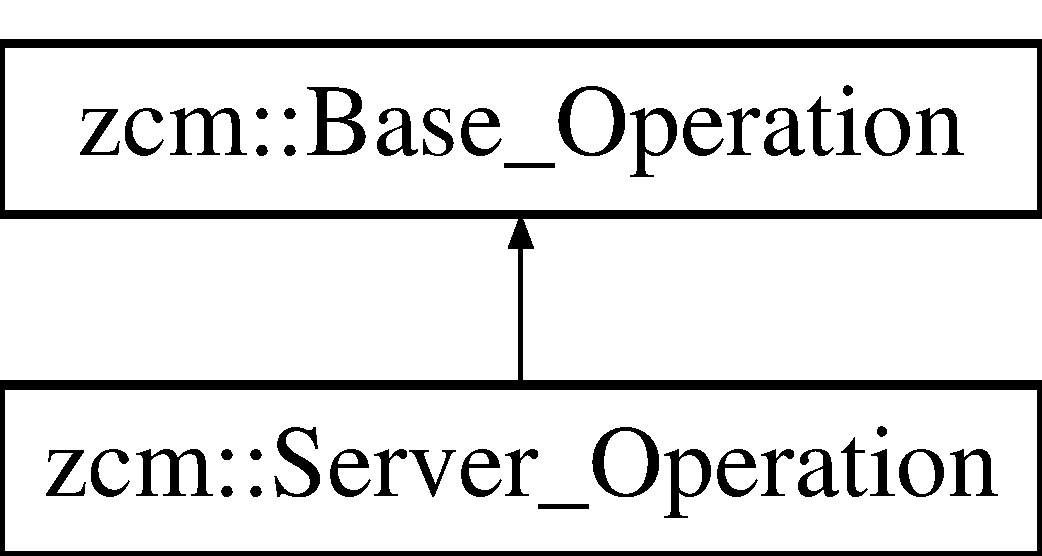
\includegraphics[height=2.000000cm]{classzcm_1_1Server__Operation}
\end{center}
\end{figure}
\subsection*{Public Member Functions}
\begin{DoxyCompactItemize}
\item 
\hyperlink{classzcm_1_1Server__Operation_a8457695fe5f8f3416106596597695406}{Server\+\_\+\+Operation} (std\+::string \hyperlink{classzcm_1_1Base__Operation_a2e2192550818d8f063fc7b2c76c5e21c}{name}, unsigned int \hyperlink{classzcm_1_1Base__Operation_a38af3bcc2578ef215772d595bf3fa358}{priority}, std\+::function$<$ std\+::string()$>$ \hyperlink{classzcm_1_1Server__Operation_a9fe0d75b858647a21323293746df6c9e}{operation\+\_\+function}, zmq\+::socket\+\_\+t $\ast$\hyperlink{classzcm_1_1Server__Operation_a07efad79c512d03a54fe2bb99166d52f}{socket\+\_\+ptr}, bool $\ast$\hyperlink{classzcm_1_1Server__Operation_a2b71778be842aedf6d122b531e186ca8}{recv\+\_\+ready})
\begin{DoxyCompactList}\small\item\em Construct a server operation. \end{DoxyCompactList}\item 
void \hyperlink{classzcm_1_1Server__Operation_acd6b89c42aad3df5dc78674770326498}{execute} ()
\begin{DoxyCompactList}\small\item\em \hyperlink{classzcm_1_1Server}{Server} operation function. \end{DoxyCompactList}\item 
zmq\+::socket\+\_\+t $\ast$ \hyperlink{classzcm_1_1Server__Operation_a17d90d76a8cfa0dc25792144e155e7c0}{get\+\_\+socket\+\_\+ptr} ()
\begin{DoxyCompactList}\small\item\em Get the Z\+MQ server socket pointer. \end{DoxyCompactList}\item 
void \hyperlink{classzcm_1_1Server__Operation_a1477e76e1639bdebc6b855d3be4e9fb2}{set\+\_\+ready} ()
\begin{DoxyCompactList}\small\item\em Get the Z\+MQ server \char`\"{}ready\char`\"{} variable. \end{DoxyCompactList}\item 
std\+::string \hyperlink{classzcm_1_1Base__Operation_a46b6a3f23e18bc35425ec2dab80c849f}{get\+\_\+name} ()
\begin{DoxyCompactList}\small\item\em Return the operation name. \end{DoxyCompactList}\item 
unsigned int \hyperlink{classzcm_1_1Base__Operation_a3b15b35c31ed173d2abb193e9fba32ef}{get\+\_\+priority} () const 
\begin{DoxyCompactList}\small\item\em Return the operation priority. \end{DoxyCompactList}\end{DoxyCompactItemize}
\subsection*{Private Attributes}
\begin{DoxyCompactItemize}
\item 
std\+::function$<$ std\+::string()$>$ \hyperlink{classzcm_1_1Server__Operation_a9fe0d75b858647a21323293746df6c9e}{operation\+\_\+function}
\begin{DoxyCompactList}\small\item\em \hyperlink{classzcm_1_1Server}{Server} Operation Function. \end{DoxyCompactList}\item 
zmq\+::socket\+\_\+t $\ast$ \hyperlink{classzcm_1_1Server__Operation_a07efad79c512d03a54fe2bb99166d52f}{socket\+\_\+ptr}
\begin{DoxyCompactList}\small\item\em Pointer to the \hyperlink{classzcm_1_1Server}{Server} Z\+MQ socket. \end{DoxyCompactList}\item 
bool $\ast$ \hyperlink{classzcm_1_1Server__Operation_a2b71778be842aedf6d122b531e186ca8}{recv\+\_\+ready}
\begin{DoxyCompactList}\small\item\em Pointer to the \hyperlink{classzcm_1_1Server}{Server} \char`\"{}ready\char`\"{} variable. \end{DoxyCompactList}\end{DoxyCompactItemize}


\subsection{Detailed Description}
\hyperlink{classzcm_1_1Server}{Server} Operation class. 

\subsection{Constructor \& Destructor Documentation}
\index{zcm\+::\+Server\+\_\+\+Operation@{zcm\+::\+Server\+\_\+\+Operation}!Server\+\_\+\+Operation@{Server\+\_\+\+Operation}}
\index{Server\+\_\+\+Operation@{Server\+\_\+\+Operation}!zcm\+::\+Server\+\_\+\+Operation@{zcm\+::\+Server\+\_\+\+Operation}}
\subsubsection[{\texorpdfstring{Server\+\_\+\+Operation(std\+::string name, unsigned int priority, std\+::function$<$ std\+::string()$>$ operation\+\_\+function, zmq\+::socket\+\_\+t $\ast$socket\+\_\+ptr, bool $\ast$recv\+\_\+ready)}{Server_Operation(std::string name, unsigned int priority, std::function< std::string()> operation_function, zmq::socket_t *socket_ptr, bool *recv_ready)}}]{\setlength{\rightskip}{0pt plus 5cm}zcm\+::\+Server\+\_\+\+Operation\+::\+Server\+\_\+\+Operation (
\begin{DoxyParamCaption}
\item[{std\+::string}]{name, }
\item[{unsigned int}]{priority, }
\item[{std\+::function$<$ std\+::string()$>$}]{operation\+\_\+function, }
\item[{zmq\+::socket\+\_\+t $\ast$}]{socket\+\_\+ptr, }
\item[{bool $\ast$}]{recv\+\_\+ready}
\end{DoxyParamCaption}
)\hspace{0.3cm}{\ttfamily [inline]}}\hypertarget{classzcm_1_1Server__Operation_a8457695fe5f8f3416106596597695406}{}\label{classzcm_1_1Server__Operation_a8457695fe5f8f3416106596597695406}


Construct a server operation. 


\begin{DoxyParams}[1]{Parameters}
\mbox{\tt in}  & {\em name} & Name of the operation \\
\hline
\mbox{\tt in}  & {\em priority} & Priority of the operation \\
\hline
\mbox{\tt in}  & {\em operation\+\_\+function} & \hyperlink{classzcm_1_1Server}{Server} function \\
\hline
\mbox{\tt in}  & {\em socket\+\_\+ptr} & Pointer to the \hyperlink{classzcm_1_1Server}{Server} Z\+MQ socket \\
\hline
\mbox{\tt in}  & {\em recv\+\_\+ready} & Pointer to the \hyperlink{classzcm_1_1Server}{Server} ready variable \\
\hline
\end{DoxyParams}


\subsection{Member Function Documentation}
\index{zcm\+::\+Server\+\_\+\+Operation@{zcm\+::\+Server\+\_\+\+Operation}!execute@{execute}}
\index{execute@{execute}!zcm\+::\+Server\+\_\+\+Operation@{zcm\+::\+Server\+\_\+\+Operation}}
\subsubsection[{\texorpdfstring{execute()}{execute()}}]{\setlength{\rightskip}{0pt plus 5cm}void zcm\+::\+Server\+\_\+\+Operation\+::execute (
\begin{DoxyParamCaption}
{}
\end{DoxyParamCaption}
)\hspace{0.3cm}{\ttfamily [virtual]}}\hypertarget{classzcm_1_1Server__Operation_acd6b89c42aad3df5dc78674770326498}{}\label{classzcm_1_1Server__Operation_acd6b89c42aad3df5dc78674770326498}


\hyperlink{classzcm_1_1Server}{Server} operation function. 



Reimplemented from \hyperlink{classzcm_1_1Base__Operation_a58cb533edd6e6f220d2d1c260fbddca4}{zcm\+::\+Base\+\_\+\+Operation}.

\index{zcm\+::\+Server\+\_\+\+Operation@{zcm\+::\+Server\+\_\+\+Operation}!get\+\_\+name@{get\+\_\+name}}
\index{get\+\_\+name@{get\+\_\+name}!zcm\+::\+Server\+\_\+\+Operation@{zcm\+::\+Server\+\_\+\+Operation}}
\subsubsection[{\texorpdfstring{get\+\_\+name()}{get_name()}}]{\setlength{\rightskip}{0pt plus 5cm}std\+::string zcm\+::\+Base\+\_\+\+Operation\+::get\+\_\+name (
\begin{DoxyParamCaption}
{}
\end{DoxyParamCaption}
)\hspace{0.3cm}{\ttfamily [inherited]}}\hypertarget{classzcm_1_1Base__Operation_a46b6a3f23e18bc35425ec2dab80c849f}{}\label{classzcm_1_1Base__Operation_a46b6a3f23e18bc35425ec2dab80c849f}


Return the operation name. 

\begin{DoxyReturn}{Returns}
Name of the operation 
\end{DoxyReturn}
\index{zcm\+::\+Server\+\_\+\+Operation@{zcm\+::\+Server\+\_\+\+Operation}!get\+\_\+priority@{get\+\_\+priority}}
\index{get\+\_\+priority@{get\+\_\+priority}!zcm\+::\+Server\+\_\+\+Operation@{zcm\+::\+Server\+\_\+\+Operation}}
\subsubsection[{\texorpdfstring{get\+\_\+priority() const }{get_priority() const }}]{\setlength{\rightskip}{0pt plus 5cm}unsigned int zcm\+::\+Base\+\_\+\+Operation\+::get\+\_\+priority (
\begin{DoxyParamCaption}
{}
\end{DoxyParamCaption}
) const\hspace{0.3cm}{\ttfamily [inherited]}}\hypertarget{classzcm_1_1Base__Operation_a3b15b35c31ed173d2abb193e9fba32ef}{}\label{classzcm_1_1Base__Operation_a3b15b35c31ed173d2abb193e9fba32ef}


Return the operation priority. 

\begin{DoxyReturn}{Returns}
Priority of the operation 
\end{DoxyReturn}
\index{zcm\+::\+Server\+\_\+\+Operation@{zcm\+::\+Server\+\_\+\+Operation}!get\+\_\+socket\+\_\+ptr@{get\+\_\+socket\+\_\+ptr}}
\index{get\+\_\+socket\+\_\+ptr@{get\+\_\+socket\+\_\+ptr}!zcm\+::\+Server\+\_\+\+Operation@{zcm\+::\+Server\+\_\+\+Operation}}
\subsubsection[{\texorpdfstring{get\+\_\+socket\+\_\+ptr()}{get_socket_ptr()}}]{\setlength{\rightskip}{0pt plus 5cm}zmq\+::socket\+\_\+t $\ast$ zcm\+::\+Server\+\_\+\+Operation\+::get\+\_\+socket\+\_\+ptr (
\begin{DoxyParamCaption}
{}
\end{DoxyParamCaption}
)}\hypertarget{classzcm_1_1Server__Operation_a17d90d76a8cfa0dc25792144e155e7c0}{}\label{classzcm_1_1Server__Operation_a17d90d76a8cfa0dc25792144e155e7c0}


Get the Z\+MQ server socket pointer. 

\index{zcm\+::\+Server\+\_\+\+Operation@{zcm\+::\+Server\+\_\+\+Operation}!set\+\_\+ready@{set\+\_\+ready}}
\index{set\+\_\+ready@{set\+\_\+ready}!zcm\+::\+Server\+\_\+\+Operation@{zcm\+::\+Server\+\_\+\+Operation}}
\subsubsection[{\texorpdfstring{set\+\_\+ready()}{set_ready()}}]{\setlength{\rightskip}{0pt plus 5cm}void zcm\+::\+Server\+\_\+\+Operation\+::set\+\_\+ready (
\begin{DoxyParamCaption}
{}
\end{DoxyParamCaption}
)}\hypertarget{classzcm_1_1Server__Operation_a1477e76e1639bdebc6b855d3be4e9fb2}{}\label{classzcm_1_1Server__Operation_a1477e76e1639bdebc6b855d3be4e9fb2}


Get the Z\+MQ server \char`\"{}ready\char`\"{} variable. 



\subsection{Member Data Documentation}
\index{zcm\+::\+Server\+\_\+\+Operation@{zcm\+::\+Server\+\_\+\+Operation}!operation\+\_\+function@{operation\+\_\+function}}
\index{operation\+\_\+function@{operation\+\_\+function}!zcm\+::\+Server\+\_\+\+Operation@{zcm\+::\+Server\+\_\+\+Operation}}
\subsubsection[{\texorpdfstring{operation\+\_\+function}{operation_function}}]{\setlength{\rightskip}{0pt plus 5cm}std\+::function$<$std\+::string()$>$ zcm\+::\+Server\+\_\+\+Operation\+::operation\+\_\+function\hspace{0.3cm}{\ttfamily [private]}}\hypertarget{classzcm_1_1Server__Operation_a9fe0d75b858647a21323293746df6c9e}{}\label{classzcm_1_1Server__Operation_a9fe0d75b858647a21323293746df6c9e}


\hyperlink{classzcm_1_1Server}{Server} Operation Function. 

\index{zcm\+::\+Server\+\_\+\+Operation@{zcm\+::\+Server\+\_\+\+Operation}!recv\+\_\+ready@{recv\+\_\+ready}}
\index{recv\+\_\+ready@{recv\+\_\+ready}!zcm\+::\+Server\+\_\+\+Operation@{zcm\+::\+Server\+\_\+\+Operation}}
\subsubsection[{\texorpdfstring{recv\+\_\+ready}{recv_ready}}]{\setlength{\rightskip}{0pt plus 5cm}bool$\ast$ zcm\+::\+Server\+\_\+\+Operation\+::recv\+\_\+ready\hspace{0.3cm}{\ttfamily [private]}}\hypertarget{classzcm_1_1Server__Operation_a2b71778be842aedf6d122b531e186ca8}{}\label{classzcm_1_1Server__Operation_a2b71778be842aedf6d122b531e186ca8}


Pointer to the \hyperlink{classzcm_1_1Server}{Server} \char`\"{}ready\char`\"{} variable. 

\index{zcm\+::\+Server\+\_\+\+Operation@{zcm\+::\+Server\+\_\+\+Operation}!socket\+\_\+ptr@{socket\+\_\+ptr}}
\index{socket\+\_\+ptr@{socket\+\_\+ptr}!zcm\+::\+Server\+\_\+\+Operation@{zcm\+::\+Server\+\_\+\+Operation}}
\subsubsection[{\texorpdfstring{socket\+\_\+ptr}{socket_ptr}}]{\setlength{\rightskip}{0pt plus 5cm}zmq\+::socket\+\_\+t$\ast$ zcm\+::\+Server\+\_\+\+Operation\+::socket\+\_\+ptr\hspace{0.3cm}{\ttfamily [private]}}\hypertarget{classzcm_1_1Server__Operation_a07efad79c512d03a54fe2bb99166d52f}{}\label{classzcm_1_1Server__Operation_a07efad79c512d03a54fe2bb99166d52f}


Pointer to the \hyperlink{classzcm_1_1Server}{Server} Z\+MQ socket. 



The documentation for this class was generated from the following files\+:\begin{DoxyCompactItemize}
\item 
/home/pranav/\+Repositories/zcm/include/\hyperlink{operation__types_8hpp}{operation\+\_\+types.\+hpp}\item 
/home/pranav/\+Repositories/zcm/src/\hyperlink{operation__types_8cpp}{operation\+\_\+types.\+cpp}\end{DoxyCompactItemize}

\hypertarget{classzcm_1_1Subscriber}{\section{zcm\-:\-:Subscriber Class Reference}
\label{classzcm_1_1Subscriber}\index{zcm\-::\-Subscriber@{zcm\-::\-Subscriber}}
}


\hyperlink{classzcm_1_1Subscriber}{Subscriber} class.  




{\ttfamily \#include $<$subscriber.\-hpp$>$}

\subsection*{Public Member Functions}
\begin{DoxyCompactItemize}
\item 
\hyperlink{classzcm_1_1Subscriber_a8477e4359c83f009ad34bbbd5e0c7b68}{Subscriber} (std\-::string \hyperlink{classzcm_1_1Subscriber_a2ec3b22204d0f3f72e996b19b086910b}{name}, unsigned int \hyperlink{classzcm_1_1Subscriber_a208baedba808c9229887ab8af00725fd}{priority}, zmq\-::context\-\_\-t $\ast$actor\-\_\-context, std\-::string \hyperlink{classzcm_1_1Subscriber_a28ab0921d97bc4d05ac6bb64c977cc35}{filter}, std\-::function$<$ void()$>$ \hyperlink{classzcm_1_1Subscriber_ab8e52c24d7dc57b33d2c1536de4197b2}{operation\-\_\-function}, \hyperlink{classzcm_1_1Operation__Queue}{Operation\-\_\-\-Queue} $\ast$\hyperlink{classzcm_1_1Subscriber_a1cd579aa570832f9656b9fa24747dde3}{operation\-\_\-queue\-\_\-ptr})
\begin{DoxyCompactList}\small\item\em Construct a subscriber object. \end{DoxyCompactList}\item 
\hyperlink{classzcm_1_1Subscriber_a248ea0aab7fc2d283f5373e33abd7287}{Subscriber} (std\-::string \hyperlink{classzcm_1_1Subscriber_a2ec3b22204d0f3f72e996b19b086910b}{name}, unsigned int \hyperlink{classzcm_1_1Subscriber_a208baedba808c9229887ab8af00725fd}{priority}, zmq\-::context\-\_\-t $\ast$actor\-\_\-context, std\-::string \hyperlink{classzcm_1_1Subscriber_a28ab0921d97bc4d05ac6bb64c977cc35}{filter}, std\-::vector$<$ std\-::string $>$ \hyperlink{classzcm_1_1Subscriber_a81590d7017038d6f50073baaa485a1b7}{endpoints}, std\-::function$<$ void()$>$ \hyperlink{classzcm_1_1Subscriber_ab8e52c24d7dc57b33d2c1536de4197b2}{operation\-\_\-function}, \hyperlink{classzcm_1_1Operation__Queue}{Operation\-\_\-\-Queue} $\ast$\hyperlink{classzcm_1_1Subscriber_a1cd579aa570832f9656b9fa24747dde3}{operation\-\_\-queue\-\_\-ptr})
\begin{DoxyCompactList}\small\item\em Construct a subscriber object with known endpoints. \end{DoxyCompactList}\item 
\hyperlink{classzcm_1_1Subscriber_a6f647c7d9f952e07b22b3aa4b63778e7}{$\sim$\-Subscriber} ()
\begin{DoxyCompactList}\small\item\em Close the subscriber socket and destroy the Z\-M\-Q context. \end{DoxyCompactList}\item 
void \hyperlink{classzcm_1_1Subscriber_a542674cff70f8d22b490a6b4a87476fe}{connect} (std\-::vector$<$ std\-::string $>$ new\-\_\-endpoints)
\begin{DoxyCompactList}\small\item\em Connect to a new set of endpoints param\mbox{[}in\mbox{]} new\-\_\-endpoints A new vector of endpoints to connect to. \end{DoxyCompactList}\item 
std\-::string \hyperlink{classzcm_1_1Subscriber_a013f450dff91644668a84cdb65d51b53}{get\-\_\-name} ()
\begin{DoxyCompactList}\small\item\em Get the name of the subscriber. \end{DoxyCompactList}\item 
unsigned int \hyperlink{classzcm_1_1Subscriber_a67427b093be45c979b4f091e6a9831ab}{get\-\_\-priority} ()
\begin{DoxyCompactList}\small\item\em Get the priority of the subscriber. \end{DoxyCompactList}\item 
void \hyperlink{classzcm_1_1Subscriber_acbfe7d4ab1b4a6fad5d9a7cbd3b8ee09}{add\-\_\-connection} (std\-::string new\-\_\-connection)
\begin{DoxyCompactList}\small\item\em Add a new connection to the subscriber. \end{DoxyCompactList}\item 
void \hyperlink{classzcm_1_1Subscriber_a3e270344beb730e009d48b04792e5526}{recv} ()
\begin{DoxyCompactList}\small\item\em Thread function of the subscriber Behavior\-: (1) Wait for a new message on the subscriber Z\-M\-Q socket (2) Create a Susbcriber Operation (3) Enqueue onto operation\-\_\-queue (4) Goto step (1) \end{DoxyCompactList}\item 
void \hyperlink{classzcm_1_1Subscriber_a43497c10d058c40395b5541a20649816}{rebind\-\_\-operation\-\_\-function} (std\-::function$<$ void()$>$ new\-\_\-operation\-\_\-function)
\begin{DoxyCompactList}\small\item\em Rebind the subscriber operation function. \end{DoxyCompactList}\item 
std\-::thread \hyperlink{classzcm_1_1Subscriber_a05334a6b27ce47e46ad525c2fc015347}{spawn} ()
\begin{DoxyCompactList}\small\item\em Spawn a new thread for the subscriber. \end{DoxyCompactList}\item 
void \hyperlink{classzcm_1_1Subscriber_af255252bdc1808c7436208b919612a48}{start} ()
\begin{DoxyCompactList}\small\item\em Start the subscriber thread. \end{DoxyCompactList}\item 
bool \hyperlink{classzcm_1_1Subscriber_adabba1785e367df820f011fbdb2a52c2}{is\-\_\-buffer\-\_\-empty} ()
\begin{DoxyCompactList}\small\item\em Is the message buffer empty? \end{DoxyCompactList}\item 
std\-::string \hyperlink{classzcm_1_1Subscriber_a153a90da1c97e12da900d02b3726a207}{message} ()
\begin{DoxyCompactList}\small\item\em Is the message buffer empty? \end{DoxyCompactList}\end{DoxyCompactItemize}
\subsection*{Private Attributes}
\begin{DoxyCompactItemize}
\item 
std\-::string \hyperlink{classzcm_1_1Subscriber_a2ec3b22204d0f3f72e996b19b086910b}{name}
\begin{DoxyCompactList}\small\item\em Name of the subscriber. \end{DoxyCompactList}\item 
unsigned int \hyperlink{classzcm_1_1Subscriber_a208baedba808c9229887ab8af00725fd}{priority}
\begin{DoxyCompactList}\small\item\em Priority of the subscriber. \end{DoxyCompactList}\item 
zmq\-::context\-\_\-t $\ast$ \hyperlink{classzcm_1_1Subscriber_a271ab3c945d1d3a84551bdca5e50f83f}{context}
\begin{DoxyCompactList}\small\item\em Pointer to the subscriber Z\-M\-Q context. \end{DoxyCompactList}\item 
std\-::string \hyperlink{classzcm_1_1Subscriber_a28ab0921d97bc4d05ac6bb64c977cc35}{filter}
\begin{DoxyCompactList}\small\item\em Reception filter enforced on all received messages. \end{DoxyCompactList}\item 
std\-::vector$<$ std\-::string $>$ \hyperlink{classzcm_1_1Subscriber_a81590d7017038d6f50073baaa485a1b7}{endpoints}
\begin{DoxyCompactList}\small\item\em Vector of connection endpoints. \end{DoxyCompactList}\item 
std\-::function$<$ void()$>$ \hyperlink{classzcm_1_1Subscriber_ab8e52c24d7dc57b33d2c1536de4197b2}{operation\-\_\-function}
\begin{DoxyCompactList}\small\item\em Operation function bound to the subscriber. \end{DoxyCompactList}\item 
\hyperlink{classzcm_1_1Operation__Queue}{Operation\-\_\-\-Queue} $\ast$ \hyperlink{classzcm_1_1Subscriber_a1cd579aa570832f9656b9fa24747dde3}{operation\-\_\-queue\-\_\-ptr}
\begin{DoxyCompactList}\small\item\em Pointer to the operation queue. \end{DoxyCompactList}\item 
zmq\-::socket\-\_\-t $\ast$ \hyperlink{classzcm_1_1Subscriber_ab6b9ee85d97a209b7c370b90882ed028}{subscriber\-\_\-socket}
\begin{DoxyCompactList}\small\item\em Pointer to the subscriber Z\-M\-Q socket. \end{DoxyCompactList}\item 
std\-::mutex \hyperlink{classzcm_1_1Subscriber_abd7e5c8f6ab6ce6e8854d8d407476c25}{func\-\_\-mutex}
\begin{DoxyCompactList}\small\item\em Mutex used to change operation\-\_\-function at runtime. \end{DoxyCompactList}\item 
std\-::queue$<$ std\-::string $>$ \hyperlink{classzcm_1_1Subscriber_a0f4c8918c98ebfdebfd46a21d6794a0b}{buffer}
\begin{DoxyCompactList}\small\item\em Buffer of messages received by the subscriber. \end{DoxyCompactList}\end{DoxyCompactItemize}


\subsection{Detailed Description}
\hyperlink{classzcm_1_1Subscriber}{Subscriber} class. 

\subsection{Constructor \& Destructor Documentation}
\hypertarget{classzcm_1_1Subscriber_a8477e4359c83f009ad34bbbd5e0c7b68}{\index{zcm\-::\-Subscriber@{zcm\-::\-Subscriber}!Subscriber@{Subscriber}}
\index{Subscriber@{Subscriber}!zcm::Subscriber@{zcm\-::\-Subscriber}}
\subsubsection[{Subscriber}]{\setlength{\rightskip}{0pt plus 5cm}zcm\-::\-Subscriber\-::\-Subscriber (
\begin{DoxyParamCaption}
\item[{std\-::string}]{name, }
\item[{unsigned int}]{priority, }
\item[{zmq\-::context\-\_\-t $\ast$}]{actor\-\_\-context, }
\item[{std\-::string}]{filter, }
\item[{std\-::function$<$ void()$>$}]{operation\-\_\-function, }
\item[{{\bf Operation\-\_\-\-Queue} $\ast$}]{operation\-\_\-queue\-\_\-ptr}
\end{DoxyParamCaption}
)\hspace{0.3cm}{\ttfamily [inline]}}}\label{classzcm_1_1Subscriber_a8477e4359c83f009ad34bbbd5e0c7b68}


Construct a subscriber object. 


\begin{DoxyParams}[1]{Parameters}
\mbox{\tt in}  & {\em name} & \hyperlink{classzcm_1_1Subscriber}{Subscriber} name \\
\hline
\mbox{\tt in}  & {\em priority} & Priority of the subscriber \\
\hline
\mbox{\tt in}  & {\em Z\-M\-Q} & Context of the \hyperlink{classzcm_1_1Actor}{Actor} Process \\
\hline
\mbox{\tt in}  & {\em filter} & Z\-M\-Q filter for the subscriber \\
\hline
\mbox{\tt in}  & {\em operation\-\_\-function} & Operation function of the subscriber \\
\hline
\mbox{\tt in}  & {\em operation\-\_\-queue\-\_\-ptr} & Pointer to the operation queue \\
\hline
\end{DoxyParams}
\hypertarget{classzcm_1_1Subscriber_a248ea0aab7fc2d283f5373e33abd7287}{\index{zcm\-::\-Subscriber@{zcm\-::\-Subscriber}!Subscriber@{Subscriber}}
\index{Subscriber@{Subscriber}!zcm::Subscriber@{zcm\-::\-Subscriber}}
\subsubsection[{Subscriber}]{\setlength{\rightskip}{0pt plus 5cm}zcm\-::\-Subscriber\-::\-Subscriber (
\begin{DoxyParamCaption}
\item[{std\-::string}]{name, }
\item[{unsigned int}]{priority, }
\item[{zmq\-::context\-\_\-t $\ast$}]{actor\-\_\-context, }
\item[{std\-::string}]{filter, }
\item[{std\-::vector$<$ std\-::string $>$}]{endpoints, }
\item[{std\-::function$<$ void()$>$}]{operation\-\_\-function, }
\item[{{\bf Operation\-\_\-\-Queue} $\ast$}]{operation\-\_\-queue\-\_\-ptr}
\end{DoxyParamCaption}
)}}\label{classzcm_1_1Subscriber_a248ea0aab7fc2d283f5373e33abd7287}


Construct a subscriber object with known endpoints. 


\begin{DoxyParams}[1]{Parameters}
\mbox{\tt in}  & {\em name} & \hyperlink{classzcm_1_1Subscriber}{Subscriber} name \\
\hline
\mbox{\tt in}  & {\em priority} & Priority of the subscriber \\
\hline
\mbox{\tt in}  & {\em Z\-M\-Q} & Context of the \hyperlink{classzcm_1_1Actor}{Actor} Process \\
\hline
\mbox{\tt in}  & {\em filter} & Z\-M\-Q filter for the subscriber \\
\hline
\mbox{\tt in}  & {\em endpoints} & A vector of endpoints to connect to \\
\hline
\mbox{\tt in}  & {\em operation\-\_\-function} & Operation function of the subscriber \\
\hline
\mbox{\tt in}  & {\em operation\-\_\-queue\-\_\-ptr} & Pointer to the operation queue \\
\hline
\end{DoxyParams}
\hypertarget{classzcm_1_1Subscriber_a6f647c7d9f952e07b22b3aa4b63778e7}{\index{zcm\-::\-Subscriber@{zcm\-::\-Subscriber}!$\sim$\-Subscriber@{$\sim$\-Subscriber}}
\index{$\sim$\-Subscriber@{$\sim$\-Subscriber}!zcm::Subscriber@{zcm\-::\-Subscriber}}
\subsubsection[{$\sim$\-Subscriber}]{\setlength{\rightskip}{0pt plus 5cm}zcm\-::\-Subscriber\-::$\sim$\-Subscriber (
\begin{DoxyParamCaption}
{}
\end{DoxyParamCaption}
)}}\label{classzcm_1_1Subscriber_a6f647c7d9f952e07b22b3aa4b63778e7}


Close the subscriber socket and destroy the Z\-M\-Q context. 



\subsection{Member Function Documentation}
\hypertarget{classzcm_1_1Subscriber_acbfe7d4ab1b4a6fad5d9a7cbd3b8ee09}{\index{zcm\-::\-Subscriber@{zcm\-::\-Subscriber}!add\-\_\-connection@{add\-\_\-connection}}
\index{add\-\_\-connection@{add\-\_\-connection}!zcm::Subscriber@{zcm\-::\-Subscriber}}
\subsubsection[{add\-\_\-connection}]{\setlength{\rightskip}{0pt plus 5cm}void zcm\-::\-Subscriber\-::add\-\_\-connection (
\begin{DoxyParamCaption}
\item[{std\-::string}]{new\-\_\-connection}
\end{DoxyParamCaption}
)}}\label{classzcm_1_1Subscriber_acbfe7d4ab1b4a6fad5d9a7cbd3b8ee09}


Add a new connection to the subscriber. 


\begin{DoxyParams}[1]{Parameters}
\mbox{\tt in}  & {\em new\-\_\-connection} & New connection address to connect to \\
\hline
\end{DoxyParams}
\hypertarget{classzcm_1_1Subscriber_a542674cff70f8d22b490a6b4a87476fe}{\index{zcm\-::\-Subscriber@{zcm\-::\-Subscriber}!connect@{connect}}
\index{connect@{connect}!zcm::Subscriber@{zcm\-::\-Subscriber}}
\subsubsection[{connect}]{\setlength{\rightskip}{0pt plus 5cm}void zcm\-::\-Subscriber\-::connect (
\begin{DoxyParamCaption}
\item[{std\-::vector$<$ std\-::string $>$}]{new\-\_\-endpoints}
\end{DoxyParamCaption}
)}}\label{classzcm_1_1Subscriber_a542674cff70f8d22b490a6b4a87476fe}


Connect to a new set of endpoints param\mbox{[}in\mbox{]} new\-\_\-endpoints A new vector of endpoints to connect to. 

\hypertarget{classzcm_1_1Subscriber_a013f450dff91644668a84cdb65d51b53}{\index{zcm\-::\-Subscriber@{zcm\-::\-Subscriber}!get\-\_\-name@{get\-\_\-name}}
\index{get\-\_\-name@{get\-\_\-name}!zcm::Subscriber@{zcm\-::\-Subscriber}}
\subsubsection[{get\-\_\-name}]{\setlength{\rightskip}{0pt plus 5cm}std\-::string zcm\-::\-Subscriber\-::get\-\_\-name (
\begin{DoxyParamCaption}
{}
\end{DoxyParamCaption}
)}}\label{classzcm_1_1Subscriber_a013f450dff91644668a84cdb65d51b53}


Get the name of the subscriber. 

\hypertarget{classzcm_1_1Subscriber_a67427b093be45c979b4f091e6a9831ab}{\index{zcm\-::\-Subscriber@{zcm\-::\-Subscriber}!get\-\_\-priority@{get\-\_\-priority}}
\index{get\-\_\-priority@{get\-\_\-priority}!zcm::Subscriber@{zcm\-::\-Subscriber}}
\subsubsection[{get\-\_\-priority}]{\setlength{\rightskip}{0pt plus 5cm}unsigned int zcm\-::\-Subscriber\-::get\-\_\-priority (
\begin{DoxyParamCaption}
{}
\end{DoxyParamCaption}
)}}\label{classzcm_1_1Subscriber_a67427b093be45c979b4f091e6a9831ab}


Get the priority of the subscriber. 

\hypertarget{classzcm_1_1Subscriber_adabba1785e367df820f011fbdb2a52c2}{\index{zcm\-::\-Subscriber@{zcm\-::\-Subscriber}!is\-\_\-buffer\-\_\-empty@{is\-\_\-buffer\-\_\-empty}}
\index{is\-\_\-buffer\-\_\-empty@{is\-\_\-buffer\-\_\-empty}!zcm::Subscriber@{zcm\-::\-Subscriber}}
\subsubsection[{is\-\_\-buffer\-\_\-empty}]{\setlength{\rightskip}{0pt plus 5cm}bool zcm\-::\-Subscriber\-::is\-\_\-buffer\-\_\-empty (
\begin{DoxyParamCaption}
{}
\end{DoxyParamCaption}
)}}\label{classzcm_1_1Subscriber_adabba1785e367df820f011fbdb2a52c2}


Is the message buffer empty? 

\hypertarget{classzcm_1_1Subscriber_a153a90da1c97e12da900d02b3726a207}{\index{zcm\-::\-Subscriber@{zcm\-::\-Subscriber}!message@{message}}
\index{message@{message}!zcm::Subscriber@{zcm\-::\-Subscriber}}
\subsubsection[{message}]{\setlength{\rightskip}{0pt plus 5cm}std\-::string zcm\-::\-Subscriber\-::message (
\begin{DoxyParamCaption}
{}
\end{DoxyParamCaption}
)}}\label{classzcm_1_1Subscriber_a153a90da1c97e12da900d02b3726a207}


Is the message buffer empty? 

\hypertarget{classzcm_1_1Subscriber_a43497c10d058c40395b5541a20649816}{\index{zcm\-::\-Subscriber@{zcm\-::\-Subscriber}!rebind\-\_\-operation\-\_\-function@{rebind\-\_\-operation\-\_\-function}}
\index{rebind\-\_\-operation\-\_\-function@{rebind\-\_\-operation\-\_\-function}!zcm::Subscriber@{zcm\-::\-Subscriber}}
\subsubsection[{rebind\-\_\-operation\-\_\-function}]{\setlength{\rightskip}{0pt plus 5cm}void zcm\-::\-Subscriber\-::rebind\-\_\-operation\-\_\-function (
\begin{DoxyParamCaption}
\item[{std\-::function$<$ void()$>$}]{new\-\_\-operation\-\_\-function}
\end{DoxyParamCaption}
)}}\label{classzcm_1_1Subscriber_a43497c10d058c40395b5541a20649816}


Rebind the subscriber operation function. 


\begin{DoxyParams}[1]{Parameters}
\mbox{\tt in}  & {\em new\-\_\-operation\-\_\-function} & New subscriber function to be handled upon \hyperlink{classzcm_1_1Subscriber_a3e270344beb730e009d48b04792e5526}{recv()} \\
\hline
\end{DoxyParams}
\hypertarget{classzcm_1_1Subscriber_a3e270344beb730e009d48b04792e5526}{\index{zcm\-::\-Subscriber@{zcm\-::\-Subscriber}!recv@{recv}}
\index{recv@{recv}!zcm::Subscriber@{zcm\-::\-Subscriber}}
\subsubsection[{recv}]{\setlength{\rightskip}{0pt plus 5cm}void zcm\-::\-Subscriber\-::recv (
\begin{DoxyParamCaption}
{}
\end{DoxyParamCaption}
)}}\label{classzcm_1_1Subscriber_a3e270344beb730e009d48b04792e5526}


Thread function of the subscriber Behavior\-: (1) Wait for a new message on the subscriber Z\-M\-Q socket (2) Create a Susbcriber Operation (3) Enqueue onto operation\-\_\-queue (4) Goto step (1) 

\hypertarget{classzcm_1_1Subscriber_a05334a6b27ce47e46ad525c2fc015347}{\index{zcm\-::\-Subscriber@{zcm\-::\-Subscriber}!spawn@{spawn}}
\index{spawn@{spawn}!zcm::Subscriber@{zcm\-::\-Subscriber}}
\subsubsection[{spawn}]{\setlength{\rightskip}{0pt plus 5cm}std\-::thread zcm\-::\-Subscriber\-::spawn (
\begin{DoxyParamCaption}
{}
\end{DoxyParamCaption}
)}}\label{classzcm_1_1Subscriber_a05334a6b27ce47e46ad525c2fc015347}


Spawn a new thread for the subscriber. 

\begin{DoxyReturn}{Returns}
\hyperlink{classzcm_1_1Subscriber}{Subscriber} thread 
\end{DoxyReturn}
\hypertarget{classzcm_1_1Subscriber_af255252bdc1808c7436208b919612a48}{\index{zcm\-::\-Subscriber@{zcm\-::\-Subscriber}!start@{start}}
\index{start@{start}!zcm::Subscriber@{zcm\-::\-Subscriber}}
\subsubsection[{start}]{\setlength{\rightskip}{0pt plus 5cm}void zcm\-::\-Subscriber\-::start (
\begin{DoxyParamCaption}
{}
\end{DoxyParamCaption}
)}}\label{classzcm_1_1Subscriber_af255252bdc1808c7436208b919612a48}


Start the subscriber thread. 



\subsection{Member Data Documentation}
\hypertarget{classzcm_1_1Subscriber_a0f4c8918c98ebfdebfd46a21d6794a0b}{\index{zcm\-::\-Subscriber@{zcm\-::\-Subscriber}!buffer@{buffer}}
\index{buffer@{buffer}!zcm::Subscriber@{zcm\-::\-Subscriber}}
\subsubsection[{buffer}]{\setlength{\rightskip}{0pt plus 5cm}std\-::queue$<$std\-::string$>$ zcm\-::\-Subscriber\-::buffer\hspace{0.3cm}{\ttfamily [private]}}}\label{classzcm_1_1Subscriber_a0f4c8918c98ebfdebfd46a21d6794a0b}


Buffer of messages received by the subscriber. 

\hypertarget{classzcm_1_1Subscriber_a271ab3c945d1d3a84551bdca5e50f83f}{\index{zcm\-::\-Subscriber@{zcm\-::\-Subscriber}!context@{context}}
\index{context@{context}!zcm::Subscriber@{zcm\-::\-Subscriber}}
\subsubsection[{context}]{\setlength{\rightskip}{0pt plus 5cm}zmq\-::context\-\_\-t$\ast$ zcm\-::\-Subscriber\-::context\hspace{0.3cm}{\ttfamily [private]}}}\label{classzcm_1_1Subscriber_a271ab3c945d1d3a84551bdca5e50f83f}


Pointer to the subscriber Z\-M\-Q context. 

\hypertarget{classzcm_1_1Subscriber_a81590d7017038d6f50073baaa485a1b7}{\index{zcm\-::\-Subscriber@{zcm\-::\-Subscriber}!endpoints@{endpoints}}
\index{endpoints@{endpoints}!zcm::Subscriber@{zcm\-::\-Subscriber}}
\subsubsection[{endpoints}]{\setlength{\rightskip}{0pt plus 5cm}std\-::vector$<$std\-::string$>$ zcm\-::\-Subscriber\-::endpoints\hspace{0.3cm}{\ttfamily [private]}}}\label{classzcm_1_1Subscriber_a81590d7017038d6f50073baaa485a1b7}


Vector of connection endpoints. 

\hypertarget{classzcm_1_1Subscriber_a28ab0921d97bc4d05ac6bb64c977cc35}{\index{zcm\-::\-Subscriber@{zcm\-::\-Subscriber}!filter@{filter}}
\index{filter@{filter}!zcm::Subscriber@{zcm\-::\-Subscriber}}
\subsubsection[{filter}]{\setlength{\rightskip}{0pt plus 5cm}std\-::string zcm\-::\-Subscriber\-::filter\hspace{0.3cm}{\ttfamily [private]}}}\label{classzcm_1_1Subscriber_a28ab0921d97bc4d05ac6bb64c977cc35}


Reception filter enforced on all received messages. 

\hypertarget{classzcm_1_1Subscriber_abd7e5c8f6ab6ce6e8854d8d407476c25}{\index{zcm\-::\-Subscriber@{zcm\-::\-Subscriber}!func\-\_\-mutex@{func\-\_\-mutex}}
\index{func\-\_\-mutex@{func\-\_\-mutex}!zcm::Subscriber@{zcm\-::\-Subscriber}}
\subsubsection[{func\-\_\-mutex}]{\setlength{\rightskip}{0pt plus 5cm}std\-::mutex zcm\-::\-Subscriber\-::func\-\_\-mutex\hspace{0.3cm}{\ttfamily [private]}}}\label{classzcm_1_1Subscriber_abd7e5c8f6ab6ce6e8854d8d407476c25}


Mutex used to change operation\-\_\-function at runtime. 

\hypertarget{classzcm_1_1Subscriber_a2ec3b22204d0f3f72e996b19b086910b}{\index{zcm\-::\-Subscriber@{zcm\-::\-Subscriber}!name@{name}}
\index{name@{name}!zcm::Subscriber@{zcm\-::\-Subscriber}}
\subsubsection[{name}]{\setlength{\rightskip}{0pt plus 5cm}std\-::string zcm\-::\-Subscriber\-::name\hspace{0.3cm}{\ttfamily [private]}}}\label{classzcm_1_1Subscriber_a2ec3b22204d0f3f72e996b19b086910b}


Name of the subscriber. 

\hypertarget{classzcm_1_1Subscriber_ab8e52c24d7dc57b33d2c1536de4197b2}{\index{zcm\-::\-Subscriber@{zcm\-::\-Subscriber}!operation\-\_\-function@{operation\-\_\-function}}
\index{operation\-\_\-function@{operation\-\_\-function}!zcm::Subscriber@{zcm\-::\-Subscriber}}
\subsubsection[{operation\-\_\-function}]{\setlength{\rightskip}{0pt plus 5cm}std\-::function$<$void()$>$ zcm\-::\-Subscriber\-::operation\-\_\-function\hspace{0.3cm}{\ttfamily [private]}}}\label{classzcm_1_1Subscriber_ab8e52c24d7dc57b33d2c1536de4197b2}


Operation function bound to the subscriber. 

\hypertarget{classzcm_1_1Subscriber_a1cd579aa570832f9656b9fa24747dde3}{\index{zcm\-::\-Subscriber@{zcm\-::\-Subscriber}!operation\-\_\-queue\-\_\-ptr@{operation\-\_\-queue\-\_\-ptr}}
\index{operation\-\_\-queue\-\_\-ptr@{operation\-\_\-queue\-\_\-ptr}!zcm::Subscriber@{zcm\-::\-Subscriber}}
\subsubsection[{operation\-\_\-queue\-\_\-ptr}]{\setlength{\rightskip}{0pt plus 5cm}{\bf Operation\-\_\-\-Queue}$\ast$ zcm\-::\-Subscriber\-::operation\-\_\-queue\-\_\-ptr\hspace{0.3cm}{\ttfamily [private]}}}\label{classzcm_1_1Subscriber_a1cd579aa570832f9656b9fa24747dde3}


Pointer to the operation queue. 

\hypertarget{classzcm_1_1Subscriber_a208baedba808c9229887ab8af00725fd}{\index{zcm\-::\-Subscriber@{zcm\-::\-Subscriber}!priority@{priority}}
\index{priority@{priority}!zcm::Subscriber@{zcm\-::\-Subscriber}}
\subsubsection[{priority}]{\setlength{\rightskip}{0pt plus 5cm}unsigned int zcm\-::\-Subscriber\-::priority\hspace{0.3cm}{\ttfamily [private]}}}\label{classzcm_1_1Subscriber_a208baedba808c9229887ab8af00725fd}


Priority of the subscriber. 

\hypertarget{classzcm_1_1Subscriber_ab6b9ee85d97a209b7c370b90882ed028}{\index{zcm\-::\-Subscriber@{zcm\-::\-Subscriber}!subscriber\-\_\-socket@{subscriber\-\_\-socket}}
\index{subscriber\-\_\-socket@{subscriber\-\_\-socket}!zcm::Subscriber@{zcm\-::\-Subscriber}}
\subsubsection[{subscriber\-\_\-socket}]{\setlength{\rightskip}{0pt plus 5cm}zmq\-::socket\-\_\-t$\ast$ zcm\-::\-Subscriber\-::subscriber\-\_\-socket\hspace{0.3cm}{\ttfamily [private]}}}\label{classzcm_1_1Subscriber_ab6b9ee85d97a209b7c370b90882ed028}


Pointer to the subscriber Z\-M\-Q socket. 



The documentation for this class was generated from the following files\-:\begin{DoxyCompactItemize}
\item 
/home/kelsier/\-Git\-Hub/zcm/include/\hyperlink{subscriber_8hpp}{subscriber.\-hpp}\item 
/home/kelsier/\-Git\-Hub/zcm/src/\hyperlink{subscriber_8cpp}{subscriber.\-cpp}\end{DoxyCompactItemize}

\hypertarget{classzcm_1_1Subscriber__Operation}{}\section{zcm\+:\+:Subscriber\+\_\+\+Operation Class Reference}
\label{classzcm_1_1Subscriber__Operation}\index{zcm\+::\+Subscriber\+\_\+\+Operation@{zcm\+::\+Subscriber\+\_\+\+Operation}}


\hyperlink{classzcm_1_1Subscriber}{Subscriber} Operation class.  




{\ttfamily \#include $<$operation\+\_\+types.\+hpp$>$}

Inheritance diagram for zcm\+:\+:Subscriber\+\_\+\+Operation\+:\begin{figure}[H]
\begin{center}
\leavevmode
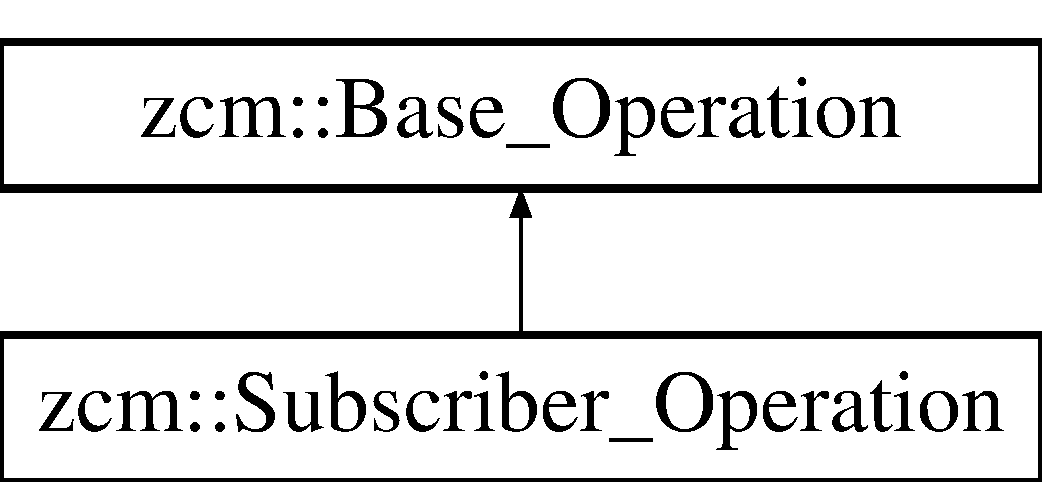
\includegraphics[height=2.000000cm]{classzcm_1_1Subscriber__Operation}
\end{center}
\end{figure}
\subsection*{Public Member Functions}
\begin{DoxyCompactItemize}
\item 
\hyperlink{classzcm_1_1Subscriber__Operation_aa0422263c6afea8bba3aa55b4c4e8c84}{Subscriber\+\_\+\+Operation} (std\+::string \hyperlink{classzcm_1_1Base__Operation_a2e2192550818d8f063fc7b2c76c5e21c}{name}, unsigned int \hyperlink{classzcm_1_1Base__Operation_a38af3bcc2578ef215772d595bf3fa358}{priority}, std\+::function$<$ void()$>$ \hyperlink{classzcm_1_1Subscriber__Operation_a5e3ca90f3ea6f1342d76f49363206e06}{operation\+\_\+function})
\begin{DoxyCompactList}\small\item\em Construct a subscriber operation. \end{DoxyCompactList}\item 
void \hyperlink{classzcm_1_1Subscriber__Operation_a2677079c7f3dd85cfc548427c1c101e6}{execute} ()
\begin{DoxyCompactList}\small\item\em \hyperlink{classzcm_1_1Subscriber}{Subscriber} operation function. \end{DoxyCompactList}\item 
std\+::string \hyperlink{classzcm_1_1Base__Operation_a46b6a3f23e18bc35425ec2dab80c849f}{get\+\_\+name} ()
\begin{DoxyCompactList}\small\item\em Return the operation name. \end{DoxyCompactList}\item 
unsigned int \hyperlink{classzcm_1_1Base__Operation_a3b15b35c31ed173d2abb193e9fba32ef}{get\+\_\+priority} () const 
\begin{DoxyCompactList}\small\item\em Return the operation priority. \end{DoxyCompactList}\end{DoxyCompactItemize}
\subsection*{Private Attributes}
\begin{DoxyCompactItemize}
\item 
std\+::function$<$ void()$>$ \hyperlink{classzcm_1_1Subscriber__Operation_a5e3ca90f3ea6f1342d76f49363206e06}{operation\+\_\+function}
\begin{DoxyCompactList}\small\item\em \hyperlink{classzcm_1_1Subscriber}{Subscriber} Operation Function. \end{DoxyCompactList}\end{DoxyCompactItemize}


\subsection{Detailed Description}
\hyperlink{classzcm_1_1Subscriber}{Subscriber} Operation class. 

\subsection{Constructor \& Destructor Documentation}
\index{zcm\+::\+Subscriber\+\_\+\+Operation@{zcm\+::\+Subscriber\+\_\+\+Operation}!Subscriber\+\_\+\+Operation@{Subscriber\+\_\+\+Operation}}
\index{Subscriber\+\_\+\+Operation@{Subscriber\+\_\+\+Operation}!zcm\+::\+Subscriber\+\_\+\+Operation@{zcm\+::\+Subscriber\+\_\+\+Operation}}
\subsubsection[{\texorpdfstring{Subscriber\+\_\+\+Operation(std\+::string name, unsigned int priority, std\+::function$<$ void()$>$ operation\+\_\+function)}{Subscriber_Operation(std::string name, unsigned int priority, std::function< void()> operation_function)}}]{\setlength{\rightskip}{0pt plus 5cm}zcm\+::\+Subscriber\+\_\+\+Operation\+::\+Subscriber\+\_\+\+Operation (
\begin{DoxyParamCaption}
\item[{std\+::string}]{name, }
\item[{unsigned int}]{priority, }
\item[{std\+::function$<$ void()$>$}]{operation\+\_\+function}
\end{DoxyParamCaption}
)\hspace{0.3cm}{\ttfamily [inline]}}\hypertarget{classzcm_1_1Subscriber__Operation_aa0422263c6afea8bba3aa55b4c4e8c84}{}\label{classzcm_1_1Subscriber__Operation_aa0422263c6afea8bba3aa55b4c4e8c84}


Construct a subscriber operation. 


\begin{DoxyParams}[1]{Parameters}
\mbox{\tt in}  & {\em name} & Name of the operation \\
\hline
\mbox{\tt in}  & {\em priority} & Priority of the operation \\
\hline
\mbox{\tt in}  & {\em operation\+\_\+function} & \hyperlink{classzcm_1_1Subscriber}{Subscriber} function \\
\hline
\end{DoxyParams}


\subsection{Member Function Documentation}
\index{zcm\+::\+Subscriber\+\_\+\+Operation@{zcm\+::\+Subscriber\+\_\+\+Operation}!execute@{execute}}
\index{execute@{execute}!zcm\+::\+Subscriber\+\_\+\+Operation@{zcm\+::\+Subscriber\+\_\+\+Operation}}
\subsubsection[{\texorpdfstring{execute()}{execute()}}]{\setlength{\rightskip}{0pt plus 5cm}void zcm\+::\+Subscriber\+\_\+\+Operation\+::execute (
\begin{DoxyParamCaption}
{}
\end{DoxyParamCaption}
)\hspace{0.3cm}{\ttfamily [virtual]}}\hypertarget{classzcm_1_1Subscriber__Operation_a2677079c7f3dd85cfc548427c1c101e6}{}\label{classzcm_1_1Subscriber__Operation_a2677079c7f3dd85cfc548427c1c101e6}


\hyperlink{classzcm_1_1Subscriber}{Subscriber} operation function. 



Reimplemented from \hyperlink{classzcm_1_1Base__Operation_a58cb533edd6e6f220d2d1c260fbddca4}{zcm\+::\+Base\+\_\+\+Operation}.

\index{zcm\+::\+Subscriber\+\_\+\+Operation@{zcm\+::\+Subscriber\+\_\+\+Operation}!get\+\_\+name@{get\+\_\+name}}
\index{get\+\_\+name@{get\+\_\+name}!zcm\+::\+Subscriber\+\_\+\+Operation@{zcm\+::\+Subscriber\+\_\+\+Operation}}
\subsubsection[{\texorpdfstring{get\+\_\+name()}{get_name()}}]{\setlength{\rightskip}{0pt plus 5cm}std\+::string zcm\+::\+Base\+\_\+\+Operation\+::get\+\_\+name (
\begin{DoxyParamCaption}
{}
\end{DoxyParamCaption}
)\hspace{0.3cm}{\ttfamily [inherited]}}\hypertarget{classzcm_1_1Base__Operation_a46b6a3f23e18bc35425ec2dab80c849f}{}\label{classzcm_1_1Base__Operation_a46b6a3f23e18bc35425ec2dab80c849f}


Return the operation name. 

\begin{DoxyReturn}{Returns}
Name of the operation 
\end{DoxyReturn}
\index{zcm\+::\+Subscriber\+\_\+\+Operation@{zcm\+::\+Subscriber\+\_\+\+Operation}!get\+\_\+priority@{get\+\_\+priority}}
\index{get\+\_\+priority@{get\+\_\+priority}!zcm\+::\+Subscriber\+\_\+\+Operation@{zcm\+::\+Subscriber\+\_\+\+Operation}}
\subsubsection[{\texorpdfstring{get\+\_\+priority() const }{get_priority() const }}]{\setlength{\rightskip}{0pt plus 5cm}unsigned int zcm\+::\+Base\+\_\+\+Operation\+::get\+\_\+priority (
\begin{DoxyParamCaption}
{}
\end{DoxyParamCaption}
) const\hspace{0.3cm}{\ttfamily [inherited]}}\hypertarget{classzcm_1_1Base__Operation_a3b15b35c31ed173d2abb193e9fba32ef}{}\label{classzcm_1_1Base__Operation_a3b15b35c31ed173d2abb193e9fba32ef}


Return the operation priority. 

\begin{DoxyReturn}{Returns}
Priority of the operation 
\end{DoxyReturn}


\subsection{Member Data Documentation}
\index{zcm\+::\+Subscriber\+\_\+\+Operation@{zcm\+::\+Subscriber\+\_\+\+Operation}!operation\+\_\+function@{operation\+\_\+function}}
\index{operation\+\_\+function@{operation\+\_\+function}!zcm\+::\+Subscriber\+\_\+\+Operation@{zcm\+::\+Subscriber\+\_\+\+Operation}}
\subsubsection[{\texorpdfstring{operation\+\_\+function}{operation_function}}]{\setlength{\rightskip}{0pt plus 5cm}std\+::function$<$void()$>$ zcm\+::\+Subscriber\+\_\+\+Operation\+::operation\+\_\+function\hspace{0.3cm}{\ttfamily [private]}}\hypertarget{classzcm_1_1Subscriber__Operation_a5e3ca90f3ea6f1342d76f49363206e06}{}\label{classzcm_1_1Subscriber__Operation_a5e3ca90f3ea6f1342d76f49363206e06}


\hyperlink{classzcm_1_1Subscriber}{Subscriber} Operation Function. 



The documentation for this class was generated from the following files\+:\begin{DoxyCompactItemize}
\item 
/home/pranav/\+Repositories/zcm/include/\hyperlink{operation__types_8hpp}{operation\+\_\+types.\+hpp}\item 
/home/pranav/\+Repositories/zcm/src/\hyperlink{operation__types_8cpp}{operation\+\_\+types.\+cpp}\end{DoxyCompactItemize}

\hypertarget{classzcm_1_1Timer}{}\section{zcm\+:\+:Timer Class Reference}
\label{classzcm_1_1Timer}\index{zcm\+::\+Timer@{zcm\+::\+Timer}}


\hyperlink{classzcm_1_1Timer}{Timer} class.  




{\ttfamily \#include $<$timer.\+hpp$>$}

\subsection*{Public Member Functions}
\begin{DoxyCompactItemize}
\item 
\hyperlink{classzcm_1_1Timer_a1283d5045e825f0f07c1cf3117eb1904}{Timer} (std\+::string \hyperlink{classzcm_1_1Timer_abfd2bb014b496ce2eda5a5837e9275f1}{name}, unsigned int \hyperlink{classzcm_1_1Timer_a722f6390254d106117d8e1545b6092ab}{priority}, long long \hyperlink{classzcm_1_1Timer_a36c7498a7ad5706ceca83429e6c1759c}{period}, std\+::function$<$ void()$>$ \hyperlink{classzcm_1_1Timer_a07f820c2d67029b83547bbfd77fc3690}{operation\+\_\+function}, \hyperlink{classzcm_1_1Operation__Queue}{Operation\+\_\+\+Queue} $\ast$\hyperlink{classzcm_1_1Timer_a9f2ce34fb9230c4251355fde956b7220}{operation\+\_\+queue\+\_\+ptr})
\begin{DoxyCompactList}\small\item\em Construct a timer. \end{DoxyCompactList}\item 
void \hyperlink{classzcm_1_1Timer_a4baed4e019656ed2612aaa0374cc0fa9}{operation} ()
\begin{DoxyCompactList}\small\item\em \hyperlink{classzcm_1_1Timer}{Timer} thread function Behavior\+: (1) Wait for timer expiry (2) Create a \hyperlink{classzcm_1_1Timer__Operation}{Timer\+\_\+\+Operation} (3) Enqueue onto operation\+\_\+queue (4) Goto step (1) \end{DoxyCompactList}\item 
std\+::string \hyperlink{classzcm_1_1Timer_a4a4aaf655539dec8ca7e747e230f8655}{get\+\_\+name} ()
\begin{DoxyCompactList}\small\item\em Get the timer name. \end{DoxyCompactList}\item 
unsigned int \hyperlink{classzcm_1_1Timer_a468548503d67c3e3872cf85d86cb26ba}{get\+\_\+priority} ()
\begin{DoxyCompactList}\small\item\em Get the timer priority. \end{DoxyCompactList}\item 
void \hyperlink{classzcm_1_1Timer_a70d8498a7fcfacc90a4510baa55682ef}{change\+\_\+period} (long long new\+\_\+period)
\begin{DoxyCompactList}\small\item\em Change the timer period. \end{DoxyCompactList}\item 
void \hyperlink{classzcm_1_1Timer_ace30a8e8155fcacf5ea8b7eee796b02b}{rebind\+\_\+operation\+\_\+function} (std\+::function$<$ void()$>$ new\+\_\+operation\+\_\+function)
\begin{DoxyCompactList}\small\item\em Rebind the timer operation function. \end{DoxyCompactList}\item 
std\+::thread \hyperlink{classzcm_1_1Timer_a05e22ac74661a4891f610e0c0d364ca7}{spawn} ()
\begin{DoxyCompactList}\small\item\em Spawn a new thread for the timer. \end{DoxyCompactList}\item 
void \hyperlink{classzcm_1_1Timer_a2a7ba9c6294a1a726844c71db962a280}{start} ()
\begin{DoxyCompactList}\small\item\em Start the timer thread. \end{DoxyCompactList}\end{DoxyCompactItemize}
\subsection*{Private Attributes}
\begin{DoxyCompactItemize}
\item 
std\+::string \hyperlink{classzcm_1_1Timer_abfd2bb014b496ce2eda5a5837e9275f1}{name}
\begin{DoxyCompactList}\small\item\em Name of the timer. \end{DoxyCompactList}\item 
unsigned int \hyperlink{classzcm_1_1Timer_a722f6390254d106117d8e1545b6092ab}{priority}
\begin{DoxyCompactList}\small\item\em Priority of the timer. \end{DoxyCompactList}\item 
std\+::chrono\+::duration$<$ long long, std\+::ratio$<$ 1, 1000000000 $>$ $>$ \hyperlink{classzcm_1_1Timer_a36c7498a7ad5706ceca83429e6c1759c}{period}
\begin{DoxyCompactList}\small\item\em Period of the timer. \end{DoxyCompactList}\item 
std\+::function$<$ void()$>$ \hyperlink{classzcm_1_1Timer_a07f820c2d67029b83547bbfd77fc3690}{operation\+\_\+function}
\begin{DoxyCompactList}\small\item\em Operation function bound to the timer. \end{DoxyCompactList}\item 
\hyperlink{classzcm_1_1Operation__Queue}{Operation\+\_\+\+Queue} $\ast$ \hyperlink{classzcm_1_1Timer_a9f2ce34fb9230c4251355fde956b7220}{operation\+\_\+queue\+\_\+ptr}
\begin{DoxyCompactList}\small\item\em Pointer to the operation queue. \end{DoxyCompactList}\item 
std\+::mutex \hyperlink{classzcm_1_1Timer_af9d6ce4df403e44b543241926ddcf41f}{period\+\_\+mutex}
\begin{DoxyCompactList}\small\item\em Mutex used to change the timer period at runtime. \end{DoxyCompactList}\item 
std\+::mutex \hyperlink{classzcm_1_1Timer_a987e7fd6128be8eac6a6a3d60c7ef9b3}{func\+\_\+mutex}
\begin{DoxyCompactList}\small\item\em Mutex used to change the operation\+\_\+function at runtime. \end{DoxyCompactList}\end{DoxyCompactItemize}


\subsection{Detailed Description}
\hyperlink{classzcm_1_1Timer}{Timer} class. 

\subsection{Constructor \& Destructor Documentation}
\index{zcm\+::\+Timer@{zcm\+::\+Timer}!Timer@{Timer}}
\index{Timer@{Timer}!zcm\+::\+Timer@{zcm\+::\+Timer}}
\subsubsection[{\texorpdfstring{Timer(std\+::string name, unsigned int priority, long long period, std\+::function$<$ void()$>$ operation\+\_\+function, Operation\+\_\+\+Queue $\ast$operation\+\_\+queue\+\_\+ptr)}{Timer(std::string name, unsigned int priority, long long period, std::function< void()> operation_function, Operation_Queue *operation_queue_ptr)}}]{\setlength{\rightskip}{0pt plus 5cm}zcm\+::\+Timer\+::\+Timer (
\begin{DoxyParamCaption}
\item[{std\+::string}]{name, }
\item[{unsigned int}]{priority, }
\item[{long long}]{period, }
\item[{std\+::function$<$ void()$>$}]{operation\+\_\+function, }
\item[{{\bf Operation\+\_\+\+Queue} $\ast$}]{operation\+\_\+queue\+\_\+ptr}
\end{DoxyParamCaption}
)}\hypertarget{classzcm_1_1Timer_a1283d5045e825f0f07c1cf3117eb1904}{}\label{classzcm_1_1Timer_a1283d5045e825f0f07c1cf3117eb1904}


Construct a timer. 


\begin{DoxyParams}[1]{Parameters}
\mbox{\tt in}  & {\em name} & Name of the timer \\
\hline
\mbox{\tt in}  & {\em priority} & Priority of the timer \\
\hline
\mbox{\tt in}  & {\em period} & Period of the timer in nanoseconds \\
\hline
\mbox{\tt in}  & {\em operation\+\_\+function} & Operation to which the timer is bound \\
\hline
\mbox{\tt in}  & {\em operation\+\_\+queue\+\_\+ptr} & Pointer to the operation\+\_\+queue \\
\hline
\end{DoxyParams}


\subsection{Member Function Documentation}
\index{zcm\+::\+Timer@{zcm\+::\+Timer}!change\+\_\+period@{change\+\_\+period}}
\index{change\+\_\+period@{change\+\_\+period}!zcm\+::\+Timer@{zcm\+::\+Timer}}
\subsubsection[{\texorpdfstring{change\+\_\+period(long long new\+\_\+period)}{change_period(long long new_period)}}]{\setlength{\rightskip}{0pt plus 5cm}void zcm\+::\+Timer\+::change\+\_\+period (
\begin{DoxyParamCaption}
\item[{long long}]{new\+\_\+period}
\end{DoxyParamCaption}
)}\hypertarget{classzcm_1_1Timer_a70d8498a7fcfacc90a4510baa55682ef}{}\label{classzcm_1_1Timer_a70d8498a7fcfacc90a4510baa55682ef}


Change the timer period. 


\begin{DoxyParams}[1]{Parameters}
\mbox{\tt in}  & {\em new\+\_\+period} & New timer period in nanoseconds \\
\hline
\end{DoxyParams}
\index{zcm\+::\+Timer@{zcm\+::\+Timer}!get\+\_\+name@{get\+\_\+name}}
\index{get\+\_\+name@{get\+\_\+name}!zcm\+::\+Timer@{zcm\+::\+Timer}}
\subsubsection[{\texorpdfstring{get\+\_\+name()}{get_name()}}]{\setlength{\rightskip}{0pt plus 5cm}std\+::string zcm\+::\+Timer\+::get\+\_\+name (
\begin{DoxyParamCaption}
{}
\end{DoxyParamCaption}
)}\hypertarget{classzcm_1_1Timer_a4a4aaf655539dec8ca7e747e230f8655}{}\label{classzcm_1_1Timer_a4a4aaf655539dec8ca7e747e230f8655}


Get the timer name. 

\begin{DoxyReturn}{Returns}
\hyperlink{classzcm_1_1Timer}{Timer} name 
\end{DoxyReturn}
\index{zcm\+::\+Timer@{zcm\+::\+Timer}!get\+\_\+priority@{get\+\_\+priority}}
\index{get\+\_\+priority@{get\+\_\+priority}!zcm\+::\+Timer@{zcm\+::\+Timer}}
\subsubsection[{\texorpdfstring{get\+\_\+priority()}{get_priority()}}]{\setlength{\rightskip}{0pt plus 5cm}unsigned int zcm\+::\+Timer\+::get\+\_\+priority (
\begin{DoxyParamCaption}
{}
\end{DoxyParamCaption}
)}\hypertarget{classzcm_1_1Timer_a468548503d67c3e3872cf85d86cb26ba}{}\label{classzcm_1_1Timer_a468548503d67c3e3872cf85d86cb26ba}


Get the timer priority. 

\begin{DoxyReturn}{Returns}
\hyperlink{classzcm_1_1Timer}{Timer} priority 
\end{DoxyReturn}
\index{zcm\+::\+Timer@{zcm\+::\+Timer}!operation@{operation}}
\index{operation@{operation}!zcm\+::\+Timer@{zcm\+::\+Timer}}
\subsubsection[{\texorpdfstring{operation()}{operation()}}]{\setlength{\rightskip}{0pt plus 5cm}void zcm\+::\+Timer\+::operation (
\begin{DoxyParamCaption}
{}
\end{DoxyParamCaption}
)}\hypertarget{classzcm_1_1Timer_a4baed4e019656ed2612aaa0374cc0fa9}{}\label{classzcm_1_1Timer_a4baed4e019656ed2612aaa0374cc0fa9}


\hyperlink{classzcm_1_1Timer}{Timer} thread function Behavior\+: (1) Wait for timer expiry (2) Create a \hyperlink{classzcm_1_1Timer__Operation}{Timer\+\_\+\+Operation} (3) Enqueue onto operation\+\_\+queue (4) Goto step (1) 

\index{zcm\+::\+Timer@{zcm\+::\+Timer}!rebind\+\_\+operation\+\_\+function@{rebind\+\_\+operation\+\_\+function}}
\index{rebind\+\_\+operation\+\_\+function@{rebind\+\_\+operation\+\_\+function}!zcm\+::\+Timer@{zcm\+::\+Timer}}
\subsubsection[{\texorpdfstring{rebind\+\_\+operation\+\_\+function(std\+::function$<$ void()$>$ new\+\_\+operation\+\_\+function)}{rebind_operation_function(std::function< void()> new_operation_function)}}]{\setlength{\rightskip}{0pt plus 5cm}void zcm\+::\+Timer\+::rebind\+\_\+operation\+\_\+function (
\begin{DoxyParamCaption}
\item[{std\+::function$<$ void()$>$}]{new\+\_\+operation\+\_\+function}
\end{DoxyParamCaption}
)}\hypertarget{classzcm_1_1Timer_ace30a8e8155fcacf5ea8b7eee796b02b}{}\label{classzcm_1_1Timer_ace30a8e8155fcacf5ea8b7eee796b02b}


Rebind the timer operation function. 


\begin{DoxyParams}[1]{Parameters}
\mbox{\tt in}  & {\em new\+\_\+operation\+\_\+function} & New timer function to be handled upon expiry \\
\hline
\end{DoxyParams}
\index{zcm\+::\+Timer@{zcm\+::\+Timer}!spawn@{spawn}}
\index{spawn@{spawn}!zcm\+::\+Timer@{zcm\+::\+Timer}}
\subsubsection[{\texorpdfstring{spawn()}{spawn()}}]{\setlength{\rightskip}{0pt plus 5cm}std\+::thread zcm\+::\+Timer\+::spawn (
\begin{DoxyParamCaption}
{}
\end{DoxyParamCaption}
)}\hypertarget{classzcm_1_1Timer_a05e22ac74661a4891f610e0c0d364ca7}{}\label{classzcm_1_1Timer_a05e22ac74661a4891f610e0c0d364ca7}


Spawn a new thread for the timer. 

\begin{DoxyReturn}{Returns}
\hyperlink{classzcm_1_1Timer}{Timer} thread 
\end{DoxyReturn}
\index{zcm\+::\+Timer@{zcm\+::\+Timer}!start@{start}}
\index{start@{start}!zcm\+::\+Timer@{zcm\+::\+Timer}}
\subsubsection[{\texorpdfstring{start()}{start()}}]{\setlength{\rightskip}{0pt plus 5cm}void zcm\+::\+Timer\+::start (
\begin{DoxyParamCaption}
{}
\end{DoxyParamCaption}
)}\hypertarget{classzcm_1_1Timer_a2a7ba9c6294a1a726844c71db962a280}{}\label{classzcm_1_1Timer_a2a7ba9c6294a1a726844c71db962a280}


Start the timer thread. 



\subsection{Member Data Documentation}
\index{zcm\+::\+Timer@{zcm\+::\+Timer}!func\+\_\+mutex@{func\+\_\+mutex}}
\index{func\+\_\+mutex@{func\+\_\+mutex}!zcm\+::\+Timer@{zcm\+::\+Timer}}
\subsubsection[{\texorpdfstring{func\+\_\+mutex}{func_mutex}}]{\setlength{\rightskip}{0pt plus 5cm}std\+::mutex zcm\+::\+Timer\+::func\+\_\+mutex\hspace{0.3cm}{\ttfamily [private]}}\hypertarget{classzcm_1_1Timer_a987e7fd6128be8eac6a6a3d60c7ef9b3}{}\label{classzcm_1_1Timer_a987e7fd6128be8eac6a6a3d60c7ef9b3}


Mutex used to change the operation\+\_\+function at runtime. 

\index{zcm\+::\+Timer@{zcm\+::\+Timer}!name@{name}}
\index{name@{name}!zcm\+::\+Timer@{zcm\+::\+Timer}}
\subsubsection[{\texorpdfstring{name}{name}}]{\setlength{\rightskip}{0pt plus 5cm}std\+::string zcm\+::\+Timer\+::name\hspace{0.3cm}{\ttfamily [private]}}\hypertarget{classzcm_1_1Timer_abfd2bb014b496ce2eda5a5837e9275f1}{}\label{classzcm_1_1Timer_abfd2bb014b496ce2eda5a5837e9275f1}


Name of the timer. 

\index{zcm\+::\+Timer@{zcm\+::\+Timer}!operation\+\_\+function@{operation\+\_\+function}}
\index{operation\+\_\+function@{operation\+\_\+function}!zcm\+::\+Timer@{zcm\+::\+Timer}}
\subsubsection[{\texorpdfstring{operation\+\_\+function}{operation_function}}]{\setlength{\rightskip}{0pt plus 5cm}std\+::function$<$void()$>$ zcm\+::\+Timer\+::operation\+\_\+function\hspace{0.3cm}{\ttfamily [private]}}\hypertarget{classzcm_1_1Timer_a07f820c2d67029b83547bbfd77fc3690}{}\label{classzcm_1_1Timer_a07f820c2d67029b83547bbfd77fc3690}


Operation function bound to the timer. 

\index{zcm\+::\+Timer@{zcm\+::\+Timer}!operation\+\_\+queue\+\_\+ptr@{operation\+\_\+queue\+\_\+ptr}}
\index{operation\+\_\+queue\+\_\+ptr@{operation\+\_\+queue\+\_\+ptr}!zcm\+::\+Timer@{zcm\+::\+Timer}}
\subsubsection[{\texorpdfstring{operation\+\_\+queue\+\_\+ptr}{operation_queue_ptr}}]{\setlength{\rightskip}{0pt plus 5cm}{\bf Operation\+\_\+\+Queue}$\ast$ zcm\+::\+Timer\+::operation\+\_\+queue\+\_\+ptr\hspace{0.3cm}{\ttfamily [private]}}\hypertarget{classzcm_1_1Timer_a9f2ce34fb9230c4251355fde956b7220}{}\label{classzcm_1_1Timer_a9f2ce34fb9230c4251355fde956b7220}


Pointer to the operation queue. 

\index{zcm\+::\+Timer@{zcm\+::\+Timer}!period@{period}}
\index{period@{period}!zcm\+::\+Timer@{zcm\+::\+Timer}}
\subsubsection[{\texorpdfstring{period}{period}}]{\setlength{\rightskip}{0pt plus 5cm}std\+::chrono\+::duration$<$long long, std\+::ratio$<$1, 1000000000$>$ $>$ zcm\+::\+Timer\+::period\hspace{0.3cm}{\ttfamily [private]}}\hypertarget{classzcm_1_1Timer_a36c7498a7ad5706ceca83429e6c1759c}{}\label{classzcm_1_1Timer_a36c7498a7ad5706ceca83429e6c1759c}


Period of the timer. 

\index{zcm\+::\+Timer@{zcm\+::\+Timer}!period\+\_\+mutex@{period\+\_\+mutex}}
\index{period\+\_\+mutex@{period\+\_\+mutex}!zcm\+::\+Timer@{zcm\+::\+Timer}}
\subsubsection[{\texorpdfstring{period\+\_\+mutex}{period_mutex}}]{\setlength{\rightskip}{0pt plus 5cm}std\+::mutex zcm\+::\+Timer\+::period\+\_\+mutex\hspace{0.3cm}{\ttfamily [private]}}\hypertarget{classzcm_1_1Timer_af9d6ce4df403e44b543241926ddcf41f}{}\label{classzcm_1_1Timer_af9d6ce4df403e44b543241926ddcf41f}


Mutex used to change the timer period at runtime. 

\index{zcm\+::\+Timer@{zcm\+::\+Timer}!priority@{priority}}
\index{priority@{priority}!zcm\+::\+Timer@{zcm\+::\+Timer}}
\subsubsection[{\texorpdfstring{priority}{priority}}]{\setlength{\rightskip}{0pt plus 5cm}unsigned int zcm\+::\+Timer\+::priority\hspace{0.3cm}{\ttfamily [private]}}\hypertarget{classzcm_1_1Timer_a722f6390254d106117d8e1545b6092ab}{}\label{classzcm_1_1Timer_a722f6390254d106117d8e1545b6092ab}


Priority of the timer. 



The documentation for this class was generated from the following files\+:\begin{DoxyCompactItemize}
\item 
/home/pranav/\+Repositories/zcm/include/\hyperlink{timer_8hpp}{timer.\+hpp}\item 
/home/pranav/\+Repositories/zcm/src/\hyperlink{timer_8cpp}{timer.\+cpp}\end{DoxyCompactItemize}

\hypertarget{classzcm_1_1Timer__Operation}{}\section{zcm\+:\+:Timer\+\_\+\+Operation Class Reference}
\label{classzcm_1_1Timer__Operation}\index{zcm\+::\+Timer\+\_\+\+Operation@{zcm\+::\+Timer\+\_\+\+Operation}}


\hyperlink{classzcm_1_1Timer}{Timer} Operation class.  




{\ttfamily \#include $<$operation\+\_\+types.\+hpp$>$}

Inheritance diagram for zcm\+:\+:Timer\+\_\+\+Operation\+:\begin{figure}[H]
\begin{center}
\leavevmode
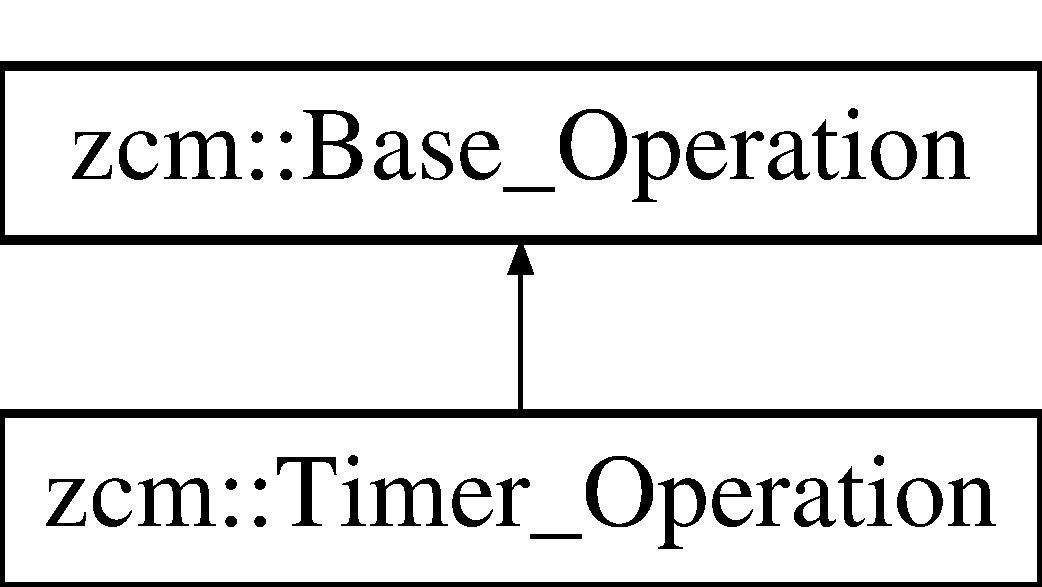
\includegraphics[height=2.000000cm]{classzcm_1_1Timer__Operation}
\end{center}
\end{figure}
\subsection*{Public Member Functions}
\begin{DoxyCompactItemize}
\item 
\hyperlink{classzcm_1_1Timer__Operation_aa578839e1aaf755f92170f20865a5740}{Timer\+\_\+\+Operation} (std\+::string \hyperlink{classzcm_1_1Base__Operation_a2e2192550818d8f063fc7b2c76c5e21c}{name}, unsigned int \hyperlink{classzcm_1_1Base__Operation_a38af3bcc2578ef215772d595bf3fa358}{priority}, std\+::function$<$ void()$>$ \hyperlink{classzcm_1_1Timer__Operation_a492e0ec6be1dfa846bbc83d9e5dea9b0}{operation\+\_\+function})
\begin{DoxyCompactList}\small\item\em Construct a timer operation. \end{DoxyCompactList}\item 
void \hyperlink{classzcm_1_1Timer__Operation_a3693312c4d4d106d0894bb35094efda7}{execute} ()
\begin{DoxyCompactList}\small\item\em \hyperlink{classzcm_1_1Timer}{Timer} operation function. \end{DoxyCompactList}\item 
std\+::string \hyperlink{classzcm_1_1Base__Operation_a46b6a3f23e18bc35425ec2dab80c849f}{get\+\_\+name} ()
\begin{DoxyCompactList}\small\item\em Return the operation name. \end{DoxyCompactList}\item 
unsigned int \hyperlink{classzcm_1_1Base__Operation_a3b15b35c31ed173d2abb193e9fba32ef}{get\+\_\+priority} () const 
\begin{DoxyCompactList}\small\item\em Return the operation priority. \end{DoxyCompactList}\end{DoxyCompactItemize}
\subsection*{Private Attributes}
\begin{DoxyCompactItemize}
\item 
std\+::function$<$ void()$>$ \hyperlink{classzcm_1_1Timer__Operation_a492e0ec6be1dfa846bbc83d9e5dea9b0}{operation\+\_\+function}
\begin{DoxyCompactList}\small\item\em \hyperlink{classzcm_1_1Timer}{Timer} operation function. \end{DoxyCompactList}\end{DoxyCompactItemize}


\subsection{Detailed Description}
\hyperlink{classzcm_1_1Timer}{Timer} Operation class. 

\subsection{Constructor \& Destructor Documentation}
\index{zcm\+::\+Timer\+\_\+\+Operation@{zcm\+::\+Timer\+\_\+\+Operation}!Timer\+\_\+\+Operation@{Timer\+\_\+\+Operation}}
\index{Timer\+\_\+\+Operation@{Timer\+\_\+\+Operation}!zcm\+::\+Timer\+\_\+\+Operation@{zcm\+::\+Timer\+\_\+\+Operation}}
\subsubsection[{\texorpdfstring{Timer\+\_\+\+Operation(std\+::string name, unsigned int priority, std\+::function$<$ void()$>$ operation\+\_\+function)}{Timer_Operation(std::string name, unsigned int priority, std::function< void()> operation_function)}}]{\setlength{\rightskip}{0pt plus 5cm}zcm\+::\+Timer\+\_\+\+Operation\+::\+Timer\+\_\+\+Operation (
\begin{DoxyParamCaption}
\item[{std\+::string}]{name, }
\item[{unsigned int}]{priority, }
\item[{std\+::function$<$ void()$>$}]{operation\+\_\+function}
\end{DoxyParamCaption}
)\hspace{0.3cm}{\ttfamily [inline]}}\hypertarget{classzcm_1_1Timer__Operation_aa578839e1aaf755f92170f20865a5740}{}\label{classzcm_1_1Timer__Operation_aa578839e1aaf755f92170f20865a5740}


Construct a timer operation. 


\begin{DoxyParams}[1]{Parameters}
\mbox{\tt in}  & {\em name} & Name of the operation \\
\hline
\mbox{\tt in}  & {\em priority} & Priority of the operation \\
\hline
\mbox{\tt in}  & {\em operation\+\_\+function} & \hyperlink{classzcm_1_1Timer}{Timer} function \\
\hline
\end{DoxyParams}


\subsection{Member Function Documentation}
\index{zcm\+::\+Timer\+\_\+\+Operation@{zcm\+::\+Timer\+\_\+\+Operation}!execute@{execute}}
\index{execute@{execute}!zcm\+::\+Timer\+\_\+\+Operation@{zcm\+::\+Timer\+\_\+\+Operation}}
\subsubsection[{\texorpdfstring{execute()}{execute()}}]{\setlength{\rightskip}{0pt plus 5cm}void zcm\+::\+Timer\+\_\+\+Operation\+::execute (
\begin{DoxyParamCaption}
{}
\end{DoxyParamCaption}
)\hspace{0.3cm}{\ttfamily [virtual]}}\hypertarget{classzcm_1_1Timer__Operation_a3693312c4d4d106d0894bb35094efda7}{}\label{classzcm_1_1Timer__Operation_a3693312c4d4d106d0894bb35094efda7}


\hyperlink{classzcm_1_1Timer}{Timer} operation function. 



Reimplemented from \hyperlink{classzcm_1_1Base__Operation_a58cb533edd6e6f220d2d1c260fbddca4}{zcm\+::\+Base\+\_\+\+Operation}.

\index{zcm\+::\+Timer\+\_\+\+Operation@{zcm\+::\+Timer\+\_\+\+Operation}!get\+\_\+name@{get\+\_\+name}}
\index{get\+\_\+name@{get\+\_\+name}!zcm\+::\+Timer\+\_\+\+Operation@{zcm\+::\+Timer\+\_\+\+Operation}}
\subsubsection[{\texorpdfstring{get\+\_\+name()}{get_name()}}]{\setlength{\rightskip}{0pt plus 5cm}std\+::string zcm\+::\+Base\+\_\+\+Operation\+::get\+\_\+name (
\begin{DoxyParamCaption}
{}
\end{DoxyParamCaption}
)\hspace{0.3cm}{\ttfamily [inherited]}}\hypertarget{classzcm_1_1Base__Operation_a46b6a3f23e18bc35425ec2dab80c849f}{}\label{classzcm_1_1Base__Operation_a46b6a3f23e18bc35425ec2dab80c849f}


Return the operation name. 

\begin{DoxyReturn}{Returns}
Name of the operation 
\end{DoxyReturn}
\index{zcm\+::\+Timer\+\_\+\+Operation@{zcm\+::\+Timer\+\_\+\+Operation}!get\+\_\+priority@{get\+\_\+priority}}
\index{get\+\_\+priority@{get\+\_\+priority}!zcm\+::\+Timer\+\_\+\+Operation@{zcm\+::\+Timer\+\_\+\+Operation}}
\subsubsection[{\texorpdfstring{get\+\_\+priority() const }{get_priority() const }}]{\setlength{\rightskip}{0pt plus 5cm}unsigned int zcm\+::\+Base\+\_\+\+Operation\+::get\+\_\+priority (
\begin{DoxyParamCaption}
{}
\end{DoxyParamCaption}
) const\hspace{0.3cm}{\ttfamily [inherited]}}\hypertarget{classzcm_1_1Base__Operation_a3b15b35c31ed173d2abb193e9fba32ef}{}\label{classzcm_1_1Base__Operation_a3b15b35c31ed173d2abb193e9fba32ef}


Return the operation priority. 

\begin{DoxyReturn}{Returns}
Priority of the operation 
\end{DoxyReturn}


\subsection{Member Data Documentation}
\index{zcm\+::\+Timer\+\_\+\+Operation@{zcm\+::\+Timer\+\_\+\+Operation}!operation\+\_\+function@{operation\+\_\+function}}
\index{operation\+\_\+function@{operation\+\_\+function}!zcm\+::\+Timer\+\_\+\+Operation@{zcm\+::\+Timer\+\_\+\+Operation}}
\subsubsection[{\texorpdfstring{operation\+\_\+function}{operation_function}}]{\setlength{\rightskip}{0pt plus 5cm}std\+::function$<$void()$>$ zcm\+::\+Timer\+\_\+\+Operation\+::operation\+\_\+function\hspace{0.3cm}{\ttfamily [private]}}\hypertarget{classzcm_1_1Timer__Operation_a492e0ec6be1dfa846bbc83d9e5dea9b0}{}\label{classzcm_1_1Timer__Operation_a492e0ec6be1dfa846bbc83d9e5dea9b0}


\hyperlink{classzcm_1_1Timer}{Timer} operation function. 



The documentation for this class was generated from the following files\+:\begin{DoxyCompactItemize}
\item 
/home/pranav/\+Repositories/zcm/include/\hyperlink{operation__types_8hpp}{operation\+\_\+types.\+hpp}\item 
/home/pranav/\+Repositories/zcm/src/\hyperlink{operation__types_8cpp}{operation\+\_\+types.\+cpp}\end{DoxyCompactItemize}

\chapter{File Documentation}
\hypertarget{actor_8hpp}{\section{/home/kelsier/\-Git\-Hub/zcm/include/actor.hpp File Reference}
\label{actor_8hpp}\index{/home/kelsier/\-Git\-Hub/zcm/include/actor.\-hpp@{/home/kelsier/\-Git\-Hub/zcm/include/actor.\-hpp}}
}


This file declares the Actor class.  


{\ttfamily \#include \char`\"{}json.\-hpp\char`\"{}}\\*
{\ttfamily \#include \char`\"{}component.\-hpp\char`\"{}}\\*
{\ttfamily \#include $<$dlfcn.\-h$>$}\\*
{\ttfamily \#include $<$fstream$>$}\\*
\subsection*{Classes}
\begin{DoxyCompactItemize}
\item 
class \hyperlink{classzcm_1_1Actor}{zcm\-::\-Actor}
\begin{DoxyCompactList}\small\item\em \hyperlink{classzcm_1_1Actor}{Actor} class. \end{DoxyCompactList}\end{DoxyCompactItemize}
\subsection*{Namespaces}
\begin{DoxyCompactItemize}
\item 
\hyperlink{namespacezcm}{zcm}
\end{DoxyCompactItemize}


\subsection{Detailed Description}
This file declares the Actor class. \begin{DoxyAuthor}{Author}
Pranav Srinivas Kumar 
\end{DoxyAuthor}
\begin{DoxyDate}{Date}
2016.\-04.\-24 
\end{DoxyDate}

\hypertarget{client_8hpp}{}\section{/home/pranav/\+Repositories/zcm/include/client.hpp File Reference}
\label{client_8hpp}\index{/home/pranav/\+Repositories/zcm/include/client.\+hpp@{/home/pranav/\+Repositories/zcm/include/client.\+hpp}}


This file declares the Client class.  


{\ttfamily \#include $<$iostream$>$}\\*
{\ttfamily \#include $<$zmq.\+hpp$>$}\\*
\subsection*{Classes}
\begin{DoxyCompactItemize}
\item 
class \hyperlink{classzcm_1_1Client}{zcm\+::\+Client}
\begin{DoxyCompactList}\small\item\em \hyperlink{classzcm_1_1Client}{Client} class. \end{DoxyCompactList}\end{DoxyCompactItemize}
\subsection*{Namespaces}
\begin{DoxyCompactItemize}
\item 
 \hyperlink{namespacezcm}{zcm}
\end{DoxyCompactItemize}


\subsection{Detailed Description}
This file declares the Client class. 

\begin{DoxyAuthor}{Author}
Pranav Srinivas Kumar 
\end{DoxyAuthor}
\begin{DoxyDate}{Date}
2016.\+04.\+24 
\end{DoxyDate}

\hypertarget{component_8hpp}{\section{/home/kelsier/\-Git\-Hub/zcm/include/component.hpp File Reference}
\label{component_8hpp}\index{/home/kelsier/\-Git\-Hub/zcm/include/component.\-hpp@{/home/kelsier/\-Git\-Hub/zcm/include/component.\-hpp}}
}


This file declares the Component class.  


{\ttfamily \#include \char`\"{}timer.\-hpp\char`\"{}}\\*
{\ttfamily \#include \char`\"{}publisher.\-hpp\char`\"{}}\\*
{\ttfamily \#include \char`\"{}subscriber.\-hpp\char`\"{}}\\*
{\ttfamily \#include \char`\"{}client.\-hpp\char`\"{}}\\*
{\ttfamily \#include \char`\"{}server.\-hpp\char`\"{}}\\*
\subsection*{Classes}
\begin{DoxyCompactItemize}
\item 
class \hyperlink{classzcm_1_1Component}{zcm\-::\-Component}
\begin{DoxyCompactList}\small\item\em \hyperlink{classzcm_1_1Component}{Component} class. \end{DoxyCompactList}\end{DoxyCompactItemize}
\subsection*{Namespaces}
\begin{DoxyCompactItemize}
\item 
\hyperlink{namespacezcm}{zcm}
\end{DoxyCompactItemize}


\subsection{Detailed Description}
This file declares the Component class. \begin{DoxyAuthor}{Author}
Pranav Srinivas Kumar 
\end{DoxyAuthor}
\begin{DoxyDate}{Date}
2016.\-04.\-24 
\end{DoxyDate}

\hypertarget{operation__queue_8hpp}{\section{/home/kelsier/\-Git\-Hub/zcm/include/operation\-\_\-queue.hpp File Reference}
\label{operation__queue_8hpp}\index{/home/kelsier/\-Git\-Hub/zcm/include/operation\-\_\-queue.\-hpp@{/home/kelsier/\-Git\-Hub/zcm/include/operation\-\_\-queue.\-hpp}}
}


This file declares the Operation\-\_\-\-Queue class.  


{\ttfamily \#include $<$iostream$>$}\\*
{\ttfamily \#include $<$queue$>$}\\*
{\ttfamily \#include $<$mutex$>$}\\*
{\ttfamily \#include $<$thread$>$}\\*
{\ttfamily \#include $<$functional$>$}\\*
{\ttfamily \#include \char`\"{}operation\-\_\-types.\-hpp\char`\"{}}\\*
\subsection*{Classes}
\begin{DoxyCompactItemize}
\item 
class \hyperlink{classzcm_1_1Operation__Queue}{zcm\-::\-Operation\-\_\-\-Queue}
\begin{DoxyCompactList}\small\item\em \hyperlink{classzcm_1_1Operation__Queue}{Operation\-\_\-\-Queue} class. \end{DoxyCompactList}\item 
struct \hyperlink{structzcm_1_1Operation__Queue_1_1PriorityOrdering}{zcm\-::\-Operation\-\_\-\-Queue\-::\-Priority\-Ordering}
\end{DoxyCompactItemize}
\subsection*{Namespaces}
\begin{DoxyCompactItemize}
\item 
\hyperlink{namespacezcm}{zcm}
\end{DoxyCompactItemize}


\subsection{Detailed Description}
This file declares the Operation\-\_\-\-Queue class. \begin{DoxyAuthor}{Author}
Pranav Srinivas Kumar 
\end{DoxyAuthor}
\begin{DoxyDate}{Date}
2016.\-04.\-24 
\end{DoxyDate}

\hypertarget{operation__types_8hpp}{\section{/home/kelsier/\-Git\-Hub/zcm/include/operation\-\_\-types.hpp File Reference}
\label{operation__types_8hpp}\index{/home/kelsier/\-Git\-Hub/zcm/include/operation\-\_\-types.\-hpp@{/home/kelsier/\-Git\-Hub/zcm/include/operation\-\_\-types.\-hpp}}
}


This file declares Operation Types.  


{\ttfamily \#include $<$iostream$>$}\\*
{\ttfamily \#include $<$functional$>$}\\*
{\ttfamily \#include \char`\"{}zmq.\-hpp\char`\"{}}\\*
\subsection*{Classes}
\begin{DoxyCompactItemize}
\item 
class \hyperlink{classzcm_1_1Base__Operation}{zcm\-::\-Base\-\_\-\-Operation}
\begin{DoxyCompactList}\small\item\em Base Operation class. \end{DoxyCompactList}\item 
class \hyperlink{classzcm_1_1Timer__Operation}{zcm\-::\-Timer\-\_\-\-Operation}
\begin{DoxyCompactList}\small\item\em \hyperlink{classzcm_1_1Timer}{Timer} Operation class. \end{DoxyCompactList}\item 
class \hyperlink{classzcm_1_1Subscriber__Operation}{zcm\-::\-Subscriber\-\_\-\-Operation}
\begin{DoxyCompactList}\small\item\em \hyperlink{classzcm_1_1Subscriber}{Subscriber} Operation class. \end{DoxyCompactList}\item 
class \hyperlink{classzcm_1_1Server__Operation}{zcm\-::\-Server\-\_\-\-Operation}
\begin{DoxyCompactList}\small\item\em \hyperlink{classzcm_1_1Server}{Server} Operation class. \end{DoxyCompactList}\end{DoxyCompactItemize}
\subsection*{Namespaces}
\begin{DoxyCompactItemize}
\item 
\hyperlink{namespacezcm}{zcm}
\end{DoxyCompactItemize}


\subsection{Detailed Description}
This file declares Operation Types. \begin{DoxyAuthor}{Author}
Pranav Srinivas Kumar 
\end{DoxyAuthor}
\begin{DoxyDate}{Date}
2016.\-04.\-24 
\end{DoxyDate}

\hypertarget{publisher_8hpp}{}\section{/home/pranav/\+Repositories/zcm/include/publisher.hpp File Reference}
\label{publisher_8hpp}\index{/home/pranav/\+Repositories/zcm/include/publisher.\+hpp@{/home/pranav/\+Repositories/zcm/include/publisher.\+hpp}}


This file declares the Publisher class.  


{\ttfamily \#include $<$iostream$>$}\\*
{\ttfamily \#include $<$zmq.\+hpp$>$}\\*
\subsection*{Classes}
\begin{DoxyCompactItemize}
\item 
class \hyperlink{classzcm_1_1Publisher}{zcm\+::\+Publisher}
\begin{DoxyCompactList}\small\item\em \hyperlink{classzcm_1_1Publisher}{Publisher} class. \end{DoxyCompactList}\end{DoxyCompactItemize}
\subsection*{Namespaces}
\begin{DoxyCompactItemize}
\item 
 \hyperlink{namespacezcm}{zcm}
\end{DoxyCompactItemize}


\subsection{Detailed Description}
This file declares the Publisher class. 

\begin{DoxyAuthor}{Author}
Pranav Srinivas Kumar 
\end{DoxyAuthor}
\begin{DoxyDate}{Date}
2016.\+04.\+24 
\end{DoxyDate}

\hypertarget{server_8hpp}{}\section{/home/pranav/\+Repositories/zcm/include/server.hpp File Reference}
\label{server_8hpp}\index{/home/pranav/\+Repositories/zcm/include/server.\+hpp@{/home/pranav/\+Repositories/zcm/include/server.\+hpp}}


This file declares the Server class.  


{\ttfamily \#include $<$iostream$>$}\\*
{\ttfamily \#include $<$vector$>$}\\*
{\ttfamily \#include $<$map$>$}\\*
{\ttfamily \#include $<$sstream$>$}\\*
{\ttfamily \#include $<$zmq.\+hpp$>$}\\*
{\ttfamily \#include \char`\"{}operation\+\_\+queue.\+hpp\char`\"{}}\\*
\subsection*{Classes}
\begin{DoxyCompactItemize}
\item 
class \hyperlink{classzcm_1_1Server}{zcm\+::\+Server}
\begin{DoxyCompactList}\small\item\em \hyperlink{classzcm_1_1Server}{Server} class. \end{DoxyCompactList}\end{DoxyCompactItemize}
\subsection*{Namespaces}
\begin{DoxyCompactItemize}
\item 
 \hyperlink{namespacezcm}{zcm}
\end{DoxyCompactItemize}


\subsection{Detailed Description}
This file declares the Server class. 

\begin{DoxyAuthor}{Author}
Pranav Srinivas Kumar 
\end{DoxyAuthor}
\begin{DoxyDate}{Date}
2016.\+04.\+24 
\end{DoxyDate}

\hypertarget{subscriber_8hpp}{\section{/home/kelsier/\-Git\-Hub/zcm/include/subscriber.hpp File Reference}
\label{subscriber_8hpp}\index{/home/kelsier/\-Git\-Hub/zcm/include/subscriber.\-hpp@{/home/kelsier/\-Git\-Hub/zcm/include/subscriber.\-hpp}}
}


This file declares the Subscriber class.  


{\ttfamily \#include $<$iostream$>$}\\*
{\ttfamily \#include $<$vector$>$}\\*
{\ttfamily \#include $<$map$>$}\\*
{\ttfamily \#include $<$sstream$>$}\\*
{\ttfamily \#include $<$zmq.\-hpp$>$}\\*
{\ttfamily \#include \char`\"{}operation\-\_\-queue.\-hpp\char`\"{}}\\*
\subsection*{Classes}
\begin{DoxyCompactItemize}
\item 
class \hyperlink{classzcm_1_1Subscriber}{zcm\-::\-Subscriber}
\begin{DoxyCompactList}\small\item\em \hyperlink{classzcm_1_1Subscriber}{Subscriber} class. \end{DoxyCompactList}\end{DoxyCompactItemize}
\subsection*{Namespaces}
\begin{DoxyCompactItemize}
\item 
\hyperlink{namespacezcm}{zcm}
\end{DoxyCompactItemize}


\subsection{Detailed Description}
This file declares the Subscriber class. \begin{DoxyAuthor}{Author}
Pranav Srinivas Kumar 
\end{DoxyAuthor}
\begin{DoxyDate}{Date}
2016.\-04.\-24 
\end{DoxyDate}

\hypertarget{timer_8hpp}{\section{/home/kelsier/\-Git\-Hub/zcm/include/timer.hpp File Reference}
\label{timer_8hpp}\index{/home/kelsier/\-Git\-Hub/zcm/include/timer.\-hpp@{/home/kelsier/\-Git\-Hub/zcm/include/timer.\-hpp}}
}


This file declares the Timer class.  


{\ttfamily \#include $<$iostream$>$}\\*
{\ttfamily \#include $<$string$>$}\\*
{\ttfamily \#include $<$chrono$>$}\\*
{\ttfamily \#include $<$ratio$>$}\\*
{\ttfamily \#include $<$thread$>$}\\*
{\ttfamily \#include \char`\"{}operation\-\_\-queue.\-hpp\char`\"{}}\\*
\subsection*{Classes}
\begin{DoxyCompactItemize}
\item 
class \hyperlink{classzcm_1_1Timer}{zcm\-::\-Timer}
\begin{DoxyCompactList}\small\item\em \hyperlink{classzcm_1_1Timer}{Timer} class. \end{DoxyCompactList}\end{DoxyCompactItemize}
\subsection*{Namespaces}
\begin{DoxyCompactItemize}
\item 
\hyperlink{namespacezcm}{zcm}
\end{DoxyCompactItemize}


\subsection{Detailed Description}
This file declares the Timer class. \begin{DoxyAuthor}{Author}
Pranav Srinivas Kumar 
\end{DoxyAuthor}
\begin{DoxyDate}{Date}
2016.\-04.\-24 
\end{DoxyDate}

\hypertarget{actor_8cpp}{\section{/home/kelsier/\-Git\-Hub/zcm/src/actor.cpp File Reference}
\label{actor_8cpp}\index{/home/kelsier/\-Git\-Hub/zcm/src/actor.\-cpp@{/home/kelsier/\-Git\-Hub/zcm/src/actor.\-cpp}}
}


This file contains definitions for the Actor class.  


{\ttfamily \#include \char`\"{}actor.\-hpp\char`\"{}}\\*
\subsection*{Namespaces}
\begin{DoxyCompactItemize}
\item 
\hyperlink{namespacezcm}{zcm}
\end{DoxyCompactItemize}


\subsection{Detailed Description}
This file contains definitions for the Actor class. \begin{DoxyAuthor}{Author}
Pranav Srinivas Kumar 
\end{DoxyAuthor}
\begin{DoxyDate}{Date}
2016.\-04.\-24 
\end{DoxyDate}

\hypertarget{client_8cpp}{\section{/home/kelsier/\-Git\-Hub/zcm/src/client.cpp File Reference}
\label{client_8cpp}\index{/home/kelsier/\-Git\-Hub/zcm/src/client.\-cpp@{/home/kelsier/\-Git\-Hub/zcm/src/client.\-cpp}}
}


This file contains definitions for the Client class.  


{\ttfamily \#include \char`\"{}client.\-hpp\char`\"{}}\\*
\subsection*{Namespaces}
\begin{DoxyCompactItemize}
\item 
\hyperlink{namespacezcm}{zcm}
\end{DoxyCompactItemize}


\subsection{Detailed Description}
This file contains definitions for the Client class. \begin{DoxyAuthor}{Author}
Pranav Srinivas Kumar 
\end{DoxyAuthor}
\begin{DoxyDate}{Date}
2016.\-04.\-24 
\end{DoxyDate}

\hypertarget{component_8cpp}{}\section{/home/pranav/\+Repositories/zcm/src/component.cpp File Reference}
\label{component_8cpp}\index{/home/pranav/\+Repositories/zcm/src/component.\+cpp@{/home/pranav/\+Repositories/zcm/src/component.\+cpp}}


This file contains definitions for the Component class.  


{\ttfamily \#include \char`\"{}component.\+hpp\char`\"{}}\\*
\subsection*{Namespaces}
\begin{DoxyCompactItemize}
\item 
 \hyperlink{namespacezcm}{zcm}
\end{DoxyCompactItemize}


\subsection{Detailed Description}
This file contains definitions for the Component class. 

\begin{DoxyAuthor}{Author}
Pranav Srinivas Kumar 
\end{DoxyAuthor}
\begin{DoxyDate}{Date}
2016.\+04.\+24 
\end{DoxyDate}

\hypertarget{operation__queue_8cpp}{\section{/home/kelsier/\-Git\-Hub/zcm/src/operation\-\_\-queue.cpp File Reference}
\label{operation__queue_8cpp}\index{/home/kelsier/\-Git\-Hub/zcm/src/operation\-\_\-queue.\-cpp@{/home/kelsier/\-Git\-Hub/zcm/src/operation\-\_\-queue.\-cpp}}
}


This file contains definitions for the Operation\-\_\-\-Queue class.  


{\ttfamily \#include \char`\"{}operation\-\_\-queue.\-hpp\char`\"{}}\\*
\subsection*{Namespaces}
\begin{DoxyCompactItemize}
\item 
\hyperlink{namespacezcm}{zcm}
\end{DoxyCompactItemize}


\subsection{Detailed Description}
This file contains definitions for the Operation\-\_\-\-Queue class. \begin{DoxyAuthor}{Author}
Pranav Srinivas Kumar 
\end{DoxyAuthor}
\begin{DoxyDate}{Date}
2016.\-04.\-24 
\end{DoxyDate}

\hypertarget{operation__types_8cpp}{\section{/home/kelsier/\-Git\-Hub/zcm/src/operation\-\_\-types.cpp File Reference}
\label{operation__types_8cpp}\index{/home/kelsier/\-Git\-Hub/zcm/src/operation\-\_\-types.\-cpp@{/home/kelsier/\-Git\-Hub/zcm/src/operation\-\_\-types.\-cpp}}
}


This file contains definitions for various Operation Types.  


{\ttfamily \#include \char`\"{}operation\-\_\-types.\-hpp\char`\"{}}\\*
\subsection*{Namespaces}
\begin{DoxyCompactItemize}
\item 
\hyperlink{namespacezcm}{zcm}
\end{DoxyCompactItemize}


\subsection{Detailed Description}
This file contains definitions for various Operation Types. \begin{DoxyAuthor}{Author}
Pranav Srinivas Kumar 
\end{DoxyAuthor}
\begin{DoxyDate}{Date}
2016.\-04.\-24 
\end{DoxyDate}

\hypertarget{publisher_8cpp}{}\section{/home/pranav/\+Repositories/zcm/src/publisher.cpp File Reference}
\label{publisher_8cpp}\index{/home/pranav/\+Repositories/zcm/src/publisher.\+cpp@{/home/pranav/\+Repositories/zcm/src/publisher.\+cpp}}


This file contains definitions for the Publisher class.  


{\ttfamily \#include \char`\"{}publisher.\+hpp\char`\"{}}\\*
\subsection*{Namespaces}
\begin{DoxyCompactItemize}
\item 
 \hyperlink{namespacezcm}{zcm}
\end{DoxyCompactItemize}


\subsection{Detailed Description}
This file contains definitions for the Publisher class. 

\begin{DoxyAuthor}{Author}
Pranav Srinivas Kumar 
\end{DoxyAuthor}
\begin{DoxyDate}{Date}
2016.\+04.\+24 
\end{DoxyDate}

\hypertarget{server_8cpp}{\section{/home/kelsier/\-Git\-Hub/zcm/src/server.cpp File Reference}
\label{server_8cpp}\index{/home/kelsier/\-Git\-Hub/zcm/src/server.\-cpp@{/home/kelsier/\-Git\-Hub/zcm/src/server.\-cpp}}
}


This file contains definitions for the Server class.  


{\ttfamily \#include \char`\"{}server.\-hpp\char`\"{}}\\*
\subsection*{Namespaces}
\begin{DoxyCompactItemize}
\item 
\hyperlink{namespacezcm}{zcm}
\end{DoxyCompactItemize}


\subsection{Detailed Description}
This file contains definitions for the Server class. \begin{DoxyAuthor}{Author}
Pranav Srinivas Kumar 
\end{DoxyAuthor}
\begin{DoxyDate}{Date}
2016.\-04.\-24 
\end{DoxyDate}

\hypertarget{subscriber_8cpp}{\section{/home/kelsier/\-Git\-Hub/zcm/src/subscriber.cpp File Reference}
\label{subscriber_8cpp}\index{/home/kelsier/\-Git\-Hub/zcm/src/subscriber.\-cpp@{/home/kelsier/\-Git\-Hub/zcm/src/subscriber.\-cpp}}
}


This file contains definitions for the Subscriber class.  


{\ttfamily \#include \char`\"{}subscriber.\-hpp\char`\"{}}\\*
\subsection*{Namespaces}
\begin{DoxyCompactItemize}
\item 
\hyperlink{namespacezcm}{zcm}
\end{DoxyCompactItemize}


\subsection{Detailed Description}
This file contains definitions for the Subscriber class. \begin{DoxyAuthor}{Author}
Pranav Srinivas Kumar 
\end{DoxyAuthor}
\begin{DoxyDate}{Date}
2016.\-04.\-24 
\end{DoxyDate}

\hypertarget{timer_8cpp}{}\section{/home/pranav/\+Repositories/zmq-\/comm/src/timer.cpp File Reference}
\label{timer_8cpp}\index{/home/pranav/\+Repositories/zmq-\/comm/src/timer.\+cpp@{/home/pranav/\+Repositories/zmq-\/comm/src/timer.\+cpp}}


This file contains definitions for the \hyperlink{classTimer}{Timer} class.  


{\ttfamily \#include \char`\"{}timer.\+hpp\char`\"{}}\\*


\subsection{Detailed Description}
This file contains definitions for the \hyperlink{classTimer}{Timer} class. 

\begin{DoxyAuthor}{Author}
Pranav Srinivas Kumar 
\end{DoxyAuthor}
\begin{DoxyDate}{Date}
2016.\+04.\+24 
\end{DoxyDate}

%--- End generated contents ---

% Index
\newpage
\phantomsection
\addcontentsline{toc}{chapter}{Index}
\printindex

\end{document}
